\chapter{Aritmetica e polinomi}\label{chapter:aritmetica}

\section{Aritmetica nell'insieme degli interi}

\subsection{Il principio di buon ordinamento}\label{sez:buonordine}

\begin{defbox}{Relazione di buon ordine}
	Sia $S$ un insieme non vuoto. Una relazione d'ordine $\leq$ in $S$ si dice una \textbf{relazione di buon ordine} se ogni parte non vuota di $S$ è dotata di minimo rispetto a $\leq$. Se $\leq$ è una relazione di buon ordine, la coppia $(S,\leq)$ si dice \textbf{insieme bene ordinato}.
\end{defbox}

\begin{lemmabox}
	Sia $S$ un insieme non vuoto, e sia $\leq$ una relazione di buon ordine in $S$. Allora $\leq$ è una relazione d'ordine totale in $S$.
\end{lemmabox}

\begin{proof}
	Siano $x$ e $y$ elementi di $S$. Allora la parte non vuota $\{x,y\}$ di $S$ è dotata di minimo $\overline{x}$, e risulta $\overline{x} = x$ oppure $\overline{x} = y$. Quindi $x \leq y$ oppure $y \leq x$, e $\leq$ è una relazione d'ordine totale per la generalità degli elementi $x,y$.
\end{proof}

\subsection{Insiemi naturalmente ordinati}
\begin{defbox}{Relazione d'ordine naturale}
	Una relazione d'ordine $\leq$ in $S$ si dice una \textbf{relazione d'ordine naturale} se ogni parte non vuota di $S$ è dotata di minimo e, se superiormente limitata, anche di massimo rispetto a $\leq$.
\end{defbox}

\begin{osservation}
	Ovviamente ogni relazione d'ordine naturale è anche una relazione di buon ordine.
\end{osservation}

Si scelga un insieme naturalmente ordinato non superiormente limitato $(\mathbb{N},\leq)$. Il Teorema sugli isomorfismi tra insiemi ordinati (Teorema \ref{thm:iso_ordinati}) assicura che, se $(S,\leq)$ è un qualunque altro insieme naturalmente ordinato non superiormente limitato esiste una applicazione biettiva e crescente $f:\mathbb{N}\rightarrow S$ sicché in particolare $\mathbb{N}$ ed $S$ sono equipotenti. Questa proprietà è sufficiente a rendere indifferente la scelta dell'insieme ordinato $(\mathbb{N},\leq)$. Gli elementi di $\mathbb{N}$ saranno chiamati \textbf{numeri naturali} ed $\mathbb{N}$ è detto \textbf{insieme dei numeri naturali}. Con il simbolo $\mathbb{N}^{*}$ denoteremo invece l'insieme dei numeri naturali positivi, ovvero:

\begin{displaymath}
	\mathbb{N}^{*} = \{1,2,3,4,5, \ldots\}
\end{displaymath}

Dimostriamo quindi il principio d'induzione introdotto nella sezione \ref{sez:induzione}. 
\begin{proof}
	Sia $X = \{n \in \mathbb{N}_{b} \; | \; \neg (p(n))\}$. Se $X \neq \emptyset$ allora, essendo $\mathbb{N}$ ben ordinato esiste il minimo di $(X,\leq)$, sia esso $m$. Si ha ovviamente che $m \neq b$ in quanto $p(b)$ è vera per ipotesi. Quindi $b \notin X$ e allora $m>b$. Tuttavia $m-1<m = min X$, dunque $m-1 \notin X$ e $p(m-1)$ risulta vera. Applicando il passo induttivo si avrebbe però:
	\begin{displaymath}
		p(m-1) \implies p((m-1)+1) = p(m)
	\end{displaymath} che è chiaramente una contraddizione rispetto alle ipotesi in quanto $p(m)$ risulta falsa. Quindi $X = \emptyset$ e per ogni $n \in \mathbb{N}_{b}$ si ha che risulta vera la proposizione $p(n)$.
\end{proof}

\begin{propbox}[Principio d'induzione - Seconda Forma]
	Per ogni $t \in \mathbb{N}_{b}$ definiamo l'insieme $M_{t}= \{x \in \mathbb{N}_{b} \; | \; x < t \} = [b,t[$. È valida la seguente implicazione:
	\begin{displaymath}
		\forall t \in \mathbb{N}_{b} \Biggl(\Bigl(\forall n \in M_{t} \bigl(p(n)\bigr) \implies p(t)\Bigr) \implies \Bigl(\forall n \in \mathbb{N}_{b}\bigl(p(n)\bigr)\Bigr)\Biggr)
	\end{displaymath}
\end{propbox}

\subsection{Divisibilità e fattorizzazione}\label{sez:associati}
Nella sezione \ref{sez:ordine} è stato introdotta la relazione di divisibilità. Sia qui $(M,\cdot,1)$ un monoide commutativo. La relazione di divisibilità in M è definita come:
\begin{equation}
	\forall a,b \in M \bigl( a \divides b \iff \exists c \in M (b=ac)\bigr)
\end{equation}

\begin{defbox}{Elementi associati}
	Per ogni $a,b \in S$ si dice che $a$ e $b$ sono \textbf{associati} e si indica con la notazione $a \sim b$ se e soltanto se:
	\begin{equation}
		(a \sim b)\iff (a \divides b \land b \divides a)
	\end{equation}
\end{defbox}

\begin{propbox}
	Se $(S,\cdot)$ è un semigruppo allora $\divides$ è una relazione transitiva.
\end{propbox}

\begin{proof}
	Per ogni $x,y,z \in S$ tali che $(x \divides y \land y \divides z)$ esistono $c,d \in S$ per i quali $(y = xc \land z = yd)$, sostituendo $y=xc$ in $z=yd$ si ottiene: $z=x(cd)$ e quindi $x \divides z$.
\end{proof}

\begin{propbox}
	Se $(S,\cdot)$ è un monoide allora $\divides$ è riflessiva.
\end{propbox}

\begin{proof}
	Preso $1_{S}$ elemento neutro in $(S,\cdot)$ si ha che per ogni $a \in S (a = a \cdot 1_{S}) \implies a \divides a$. 
\end{proof}

\begin{propbox}
	Se $(S,\cdot)$ è un monoide, la relazione di divisibilità  $\divides_{(S,\cdot)}$ è una relazione d'ordine se e soltanto se è antisimmetrica. Vale cioè:
	\[\divides_{(S,\cdot)} \in \textbf{OL(S)} \iff \forall a,b \in S (a \divides b \land b \divides a \implies a = b)\]
\end{propbox}

\begin{proof}
Abbiamo:
	\begin{itemize}
		\item[$\impliedby$] Banale
		\item[$\implies$] Siano $a,b \in S$ tali che $a \divides b$ e $b \divides a$. Per definizione di divisibilità in $S$ abbiamo:
		\begin{align*}
			\begin{cases*}
				\exists c_{1} \in S (b = a \cdot c_{1})\\	
				\exists c_{2} \in S (a = b \cdot c_{2})
			\end{cases*}
		\end{align*}
		Sostituendo l'espressione di $b$ nella seconda relazione, otteniamo:
		\begin{align*}
			a &= (a \cdot c_{1}) \cdot c_{2}\\ 
			&= a \cdot(c_{1} \cdot c_{2}) & \text{\textcolor{gray}{(Applicando l'associatività di $\cdot$ in $S$)}} \\
		\end{align*}
		Poiché $S$ è un monoide, esiste un elemento neutro $1_{S}$ tale che $a = a \cdot 1_{S}$, deve essere $(c_{1} \cdot c_{2}) = 1_{S}$ e risultano essere uno l'inverso dell'altro, e in particolare cancellabili per il Teorema \ref{thm:cancellabili}. Quindi:
		\begin{align*}
			c_{1} \cdot a = c_{1} \cdot b \implies a=b
		\end{align*}
		Quindi $\divides_{(S,\cdot)}$ è antisimmetrica.
	\end{itemize}
\end{proof}

\begin{example}
	La relazione di divisibilità in $(\mathbb{N}, \cdot)$ è di ordine largo; infatti $a \sim b \iff a=b$. Non è antisimmetrica in $(\mathbb{Z}, \cdot)$, infatti $(1 \divides -1) \land (-1 \divides 1)$ ma $-1 \neq 1$.
\end{example}

L'essere associati risulta chiaramente essere una relazione di equivalenza in quanto è:
\begin{enumerate}
	\item \textbf{Riflessiva}: $\forall a \in M$ sicuramente $a \divides a$ in quanto esiste $1 \in M$ tale che $a = 1a$;
	\item \textbf{Simmetrica}: se $a \sim b$ sicuramente $b \sim a$ per la commutatività della congiunzione;
	\item \textbf{Transitiva}: se $a \sim b$ e $b \sim c$ allora sicuramente $a \sim c$.
\end{enumerate}

\begin{propbox}
	Per ogni $a,b \in M$, siano $a \sim a'$ e $b \sim b'$. Allora:
	\begin{displaymath}
		a \divides b \iff a' \divides b'
	\end{displaymath}
\end{propbox}

\begin{proof}
	Se $a \divides b$ allora, per ipotesi, $a' \divides a$, $a \divides b$, $b \divides b'$. Quindi $a' \divides b'$ per la transitività della relazione. Il viceversa è equivalente.
\end{proof}


\begin{propbox}
	Per ogni $a,b \in M$:
	\begin{displaymath}
		a \sim b \iff Div(a)= Div(b) \iff aM = bM
	\end{displaymath}
	Ovvero: due elementi sono associati se hanno gli stessi divisori e gli stessi multipli. Infatti $Div(a) = \{ d \in M \; | \; d \divides a \}$ e $aM = \{ax \; | \; x \in M\} = \{m \in M \; | \; a \divides m \}$.
\end{propbox}

\begin{proof} Si ha:
	\begin{itemize}
		\item[$\implies$] 	Per ogni $d \in Div(a)$ da $d \divides a$ e $a \divides b$ segue $d \divides b$ per transitività. Quindi $d \in Div(b)$ e $Div(a) \subseteq Div(b)$. Chiaramente vale anche l'inclusione inversa e quindi $Div(a)= Div(b)$.
		\item[$\impliedby$] Poiché $a \in Div(a)$, se vale $Div(a)=Div(b)$ allora $a \in Div(b)$ e $a \divides b$. Similmente $b \in Div(a)$ e $b \divides a$ quindi $a \sim b$.
	\end{itemize}
\end{proof}


\begin{propbox}
	Per ogni $u \in \mathcal{U}(M)$, per ogni $a \in M$ vale: $a \sim au$.
\end{propbox}

\begin{proof}
	Si ricordi che $\mathcal{U}(M)$ è l'insieme degli elementi invertibili di $M$. Quindi per ogni $x \in \mathcal{U}(M)$ esiste $u'$ tale che $u\cdot u'=1$. Ovviamente $a \divides au$ e, se consideriamo $a = (au) u'$ allora $au \divides a$.
\end{proof}


\begin{propbox}
	Se $a$ è cancellabile in $M$ allora:
	\begin{displaymath}
		[a]_{\sim} = \{au \; | \; u \in \mathcal{U}(M)\}
	\end{displaymath}
\end{propbox}

\begin{proof}
	Per la proposizione precedente si ha che $\forall u \in \mathcal{U}(M) (a \sim au)$, quindi sicuramente $\{au \; | \; u \in \mathcal{U}(M)\} \subseteq [a]_{\sim}$. Per verificare l'uguaglianza basta completare la verifica della doppia inclusione: ovvero dimostrare che ogni elemento associato ad $a$ è della forma $au$ per un opportuno $u \in \mathcal{U}(M)$. Sia quindi $b \in M$ tale che $b \sim a$, ovvero $b \in [a]_{\sim}$. Chiaramente, per definizione di elemento associato $a \divides b$ e quindi esiste $u \in M$ tale che $b = au$. Vale inoltre $b \divides a$ e quindi esiste $v \in M$ tale che $a = bv$. Allora:
	\begin{displaymath}
		a \cdot 1_{M} = a = bv = (au)v = a (uv)
	\end{displaymath}
	Poiché $a$ è cancellabile per ipotesi deve essere $uv = 1_{M}$ e quindi $v = u^{-1}$ e $u,v \in \mathcal{U}(M)$.
\end{proof} 

\begin{osservation}
	In $\mathbb{N}$ gli elementi associati \textit{devono essere per forza uguali} in quanto esiste un solo elemento invertibile.
\end{osservation}

\begin{defbox}{Divisori banali e propri}
	Per ogni elemento $a$ in un monoide commutativo $M$, tra i divisori di $a$ ci sono:
	\begin{itemize}
		\item Gli elementi associati ad $a$;
		\item Gli elementi invertibili di $M$;
	\end{itemize}
	Chiameremo questi elementi \textbf{divisori banali}\index{Divisore!banale} di $a$.	Un divisore di un elemento $a$ si dice \textbf{proprio}\index{Divisore!proprio} se non è associato ad $a$.
\end{defbox}

\begin{defbox}{Elementi irriducibili}
	Un elemento si dice \textbf{irriducibile}\index{Elemento!irriducibile} in $(M,\cdot)$ se e solo se $a \notin \mathcal{U}(M)$ e non ha divisori propri in $M$, ovvero se:
	\begin{enumerate}
		\item $a$ non è invertibile;
		\item gli unici divisori di $a$ sono i divisori banali.
	\end{enumerate}
\end{defbox}

\begin{osservation}
	Sia $M=(\mathbb{N}^{*},\cdot)$ , gli elementi irriducibili di $M$ sono detti \textbf{numeri primi}. Tali elementi ammettono come divisori solo $1$ e sé stessi. L'elemento $1$ non è primo in quanto risulta essere invertibile in $\mathbb{N}^{*}$.
\end{osservation}

\subsubsection{Fattorizzazione in irriducibili}

\begin{teorbox}[Fondamentale dell'Aritmetica]\index{TFA}
	Sia $a \in M$. Tale elemento o è esprimibile come prodotto di elementi irriducibili oppure è esso stesso irriducibile. Inoltre se $a=p_{1}\cdot p_{2} \cdot \dots p_{t} = q_{1} \cdot q_{2} \cdot \dots q_{s}$ con $t,s \in \mathbb{N}^{*}$ e $p_{1},p_{2}, \ldots, p_{t},q_{1},q_{2},\ldots, q_{s}$ elementi irriducibili, allora $s=t$ ed esiste una permutazione $\sigma$ di $\{1,\ldots,s\}$ tale che $p_{i} = \pm q_{\sigma(i)}$ per ogni $i=1,\ldots,s$.
\end{teorbox}

\begin{defbox}{Monoide fattoriale}\index{Monoide!Fattoriale}
	Un monoide commutativo $(M,\cdot)$ si dice \textbf{fattoriale} se e solo se esso è cancellativo (ogni elemento risulta cancellabile) ed ogni elemento di $M \setminus \mathcal{U}(M)$ è prodotto di irriducibili in modo essenzialmente unico.
\end{defbox}

\begin{defbox}{Anello fattoriale}\index{Anello!fattoriale}
	Un anello non nullo $A$ si dice \textbf{fattoriale} se è un dominio di integrità unitario e se $(A\setminus \{0\},\cdot)$ è un monoide fattoriale.\footnote{$A$ può anche prendere il nome di \textbf{dominio a fattorizzazione unica}, spesso abbreviato in UFD, dall'inglese \textit{Unique Factorization Domain}.}\index{Dominio!a fattorizzazione unica}
\end{defbox}

\begin{corolbox}
	Risultano essere monoidi fattoriali: $(\mathbb{N}^{*},\cdot, 1)$, $(\mathbb{Z}\setminus\{0\},\cdot,1)$. La struttura $(\mathbb{Z},+,\cdot)$ è un anello fattoriale.
\end{corolbox}

Di questo corollario non forniremo la dimostrazione completa, bensì mostreremo che:
\begin{lemmabox}
	 Ogni intero diverso da $0$, $1$ e $-1$ è prodotto di primi.
\end{lemmabox}

\begin{proof}
	Per assurdo di supponga non vuoto l'insieme:
	\begin{displaymath}
		X \coloneqq \{n \in \mathbb{N} \; | \; n > 1 \land \text{$n$ non è prodotto di numeri primi}\}
	\end{displaymath}
	Essendo $\mathbb{N}$ un insieme ben ordinato allora esisterà il minimo di tale insieme $X$. Sia esso $m$: tale elemento risulta essere non primo, e poiché $m>1$, esso avrà qualche divisore non banale; sia $a$ uno di questi. Esisterà quindi $b \in \mathbb{N}^{*}$ per il quale $m=ab$, con $1<a<m$ e $1<b<m$. Ne segue che $a,b \notin X$ dato che $m= min(X)$. Quindi $a,b$ sono prodotti di primi e allora anche $m$ dovrà per forza esserlo.
\end{proof}

\begin{example}
	Un esempio di domini a fattorizzazione unica è dato dai campi, come il campo dei numeri razionali $\mathbb{Q}$ o reali $\mathbb {R}$: in questo caso, tutti gli elementi non nulli sono invertibili, e quindi tutte le fattorizzazioni sono banali. 
\end{example}

\begin{lemmabox}[di Gauss]\index{Gauss}
	Per ogni $p \in \mathbb{Z}$ vale la seguente implicazione:
	\begin{displaymath}
		p \in \mathbb{P} \implies \bigl(\forall a,b \in \mathbb{Z}(p \divides ab \implies p \divides a \lor p \divides b)\bigr)
	\end{displaymath}
\end{lemmabox}

\begin{proof}
	Per il Teorema Fondamentale dell'Aritmetica possiamo scrivere $a$ e $b$ come prodotti di primi:
	\begin{displaymath}
		\begin{array}{l}
			a=p_{1}\cdot p_{2}\cdot \ldots \cdot p_{n}\\
			b=q_{1}\cdot q_{2} \cdot \ldots \cdot q_{m}
		\end{array}
	\end{displaymath}
	Se per ipotesi $p \in \mathbb{P}$, dove $\mathbb{P}$ è l'insieme dei numeri primi, e $p \divides ab$ allora esiste $c \in \mathbb{Z}$ per il quale $ab = pc$ e anche $c$ risulta essere primo o prodotto di primi. Sia $c=m_{1}\cdot m_{2} \cdot \ldots m_{t}$ allora:
	\begin{displaymath}
		\underbrace{(p_{1}\cdot p_{2}\cdot \ldots \cdot p_{n})}_{a}\underbrace{(q_{1}\cdot q_{2} \cdot \ldots \cdot q_{m})}_{b} = p \underbrace{(m_{1}\cdot m_{2} \cdot \ldots \cdot m_{t})}_{c}
	\end{displaymath}
	Per l'unicità della scrittura deve essere quindi $p = p_{i}$ oppure $p=q_{j}$ per opportuni indici $i$, $j$.
\end{proof}

\begin{propbox}
	In $\mathbb{N}^{*}$ sia $a=P_{1}^{\alpha_{1}}\cdot P_{2}^{\alpha_{2}} \cdot \ldots \cdot P_{T}^{\alpha_{t}}$, dove $t \in \mathbb{N}^{*}$, per ogni $i \in \{1,\ldots,t\}$ si ha $P_{i} \in \mathbb{P}$ e $\alpha_{i}\in \mathbb{N}$. Inoltre per ogni $i \neq j$ si ha $P_{i} \neq P_{j}$. I divisori di $a $ in $\mathbb{N}^{*}$ sono tutti e soli i numeri della forma $P_{1}^{\lambda_{1}}\cdot \ldots P_{t}^{\lambda_{t}}$ dove per ogni $i \in \{1,\ldots,t\}$ si ha $\alpha_{i} \geq \lambda_{i}$. Questi divisori sono esattamente $(\alpha_{1}+1)\cdot(\alpha_{2}+1)\cdot \ldots \cdot (\alpha_{t}+1)$.
\end{propbox}

\begin{example}
	Si consideri il numero $12$ e la sua scomposizione in fattori primi: $$12 = 2^{2}\cdot3^{1}$$
	Si avrà che il numero di divisori di 12 è pari a $(2+1)(1+1)=3 \cdot 2 = 6$. Infatti $|Div(12)|=6$ ed è possibile esprimere tale insieme nella seguente forma:
	\begin{displaymath}
		Div(12) = \{2^{\lambda_{1}}\cdot 3^{\lambda_{2}}\; | \; \lambda_{1} \in \{0,1,2\} \land \lambda_{2} \in \{0,1\}\}
	\end{displaymath}
	Risultano elementi di $Div(12)$ quindi i numeri ottenuti calcolando le varie espressioni:
	\begin{displaymath}
		\begin{array}{cc}
			2^{0}\cdot 3^{0}= 1 & 2^{0}\cdot3^{1}=3  \\
			2^{1}\cdot 3^{0}= 2 & 2^{1} \cdot 3^{1}=6 \\
			2^{2}\cdot 3^{0}=4 & 2^{2}\cdot 3^{1}=12
		\end{array}
	\end{displaymath}
\end{example}

\begin{lemmabox}
	Siano $R$ un anello commutativo unitario e $a,b,c \in R$ . Allora:
	\begin{equation}
		(a \divides b \land a \divides c) \implies (\forall u,v \in R)(a \divides bu+cv)
	\end{equation}
\end{lemmabox}

\begin{proof}
	Se $a \divides b$ e $a \divides c$ esistono $\beta,\delta \in R$ tale che $b = a\beta$  e $c= a \delta$. Siano ora $u,v \in R$ e consideriamo la combinazione lineare $bv+cu$. Abbiamo allora:
	\begin{align*}
		bv+cu &= (a \beta)v + (a \delta)u \\
		&= a (\beta v) +  a (\delta u)\\
		&= a (\beta v + \delta u)
	\end{align*}
	Che risulta essere multiplo di $a$. Allora $a \divides (bv+cu)$ per ogni $u,v \in R$. Quindi se due elementi sono multipli di $a$, tutte le combinazioni lineari tra i due elementi sono multipli di $a$.
\end{proof}

\subsection{Algoritmo euclideo, MCD ed equazioni diofantee}\index{Algoritmo!Euclideo}
Se $a$ e $b$ sono numeri interi, si dice che $a$ divide $b$, in simboli $a \divides b$, se e solo se esiste $c \in \mathbb{Z}$ tale che $b=ac$. Si può subito notare che:
\begin{itemize}
	\item 1 e -1 sono gli unici interi che dividano ogni intero;
	\item 0 è l'unico intero che sia diviso da ogni intero;
	\item $\forall a,b \in \mathbb{Z} \bigl( a \divides b \iff -a \divides b \iff a \divides -b \iff -a \divides -b \bigr)$.
\end{itemize}
L'insieme dei divisori (in $\mathbb{Z}$) di un intero $n$ si indica come $D(n)$. Dunque, per ogni $n \in \mathbb{Z}$:
\begin{equation}
	D(n) \coloneqq \{a \in \mathbb{Z} \; | \; a \divides n \}
\end{equation}
\begin{defbox}{Massimo comun divisore}\index{Massimo Comun Divisore}
	Siano $a,b \in \mathbb{Z}$. Un numero $d$ si dice \textbf{massimo comune divisore} di $a$ e $b$ se:
	\begin{itemize}
		\item $d \divides a$ e $d \divides b$
		\item $\forall c \in \mathbb{Z} \bigl((c \divides a \land c \divides b) \implies c \divides d \bigr)$
	\end{itemize}
	Dunque, un massimo comun divisore tra $a$ e $b$ è un divisore comune ad $a$ e $b$ che sia diviso da ogni altro divisore comune di $a$ e $b$.
\end{defbox}

\begin{defbox}{Minimo comune multiplo}\index{Minimo Comune Multiplo}
	Siano $a$ e $b$ numeri naturali non nulli. Un numero naturale $m$ si dice \textbf{minimo comune multiplo} di $a$ e $b$ se $m$ è multiplo comune di $a$ e $b$ e inoltre divide ogni altro multiplo comune di $a$ e $b$.
\end{defbox}


Il massimo comun divisore non negativo tra due interi a e b viene spesso indicato con il simbolo $MCD(a, b)$. Se una coppia $(a,b)$ di elementi di un semigruppo commutativo regolare unitario $M$ è dotata di massimo comun divisore e di minimo comune multiplo, questi non sono necessariamente unici. Si ha però:
\begin{itemize}
	\item Se $d$ è un massimo comun divisore tra due interi $a$ e $b$, allora $d$ e $-d$ sono gli unici massimi comun divisori tra $a$ e $b$. Dunque, calcolare un MCD tra due interi equivale a calcolarli tutti.
	\item Per ogni $a,b \in \mathbb{Z}$, i divisori comuni ad $a$ e $b$ sono tutti e soli i divisori comuni ad $|a|$ e $|b|$; quindi i massimi comun divisori tra $a$ e $b$ sono tutti e soli i massimi comun divisori tra $|a|$ e $|b|$.
\end{itemize}
Il calcolo dei massimi comun divisori tra 0 ed un arbitrario intero è immediato, come segue da queste altre due osservazioni:
\begin{itemize}
	\item Se $a$ e $b$ sono interi e $a \divides b$ allora $a$ è un massimo comun divisore tra $a$ e $b$.
	\item Per ogni $a \in \mathbb{Z}$, si ha che $a$ è un massimo comun divisore tra $a$ e $0$.
\end{itemize}

\begin{osservation}
	Siano $a,b \in \mathbb{N}^{*}$ con $a=p_{1}^{\alpha_{1}}\cdot \ldots \cdot p_{t}^{\alpha_{t}}$ e $b=p_{1}^{\beta_{1}}\cdot \ldots \cdot p_{t}^{\beta_{t}}$, i divisori comuni sono i numeri della forma $p_{1}^{\lambda_{1}}\cdot \ldots \cdot p_{t}^{\lambda_{t}}$ dove per ogni $i \in \{1,\ldots,t\}$ si ha $\lambda_{i} \leq min \{\alpha_{i},\beta_{i}\} = \delta_{i}$. Allora presi gli esponenti $\delta_{i}$ così individuati, il massimo comune divisore di $a$ e $b$ è:
	\begin{displaymath}
		d = p_{1}^{\delta_{1}}\cdot \ldots \cdot p_{t}^{\delta_{t}}
	\end{displaymath}
	Analogamente, scelto $u_{i}=max\{\alpha_{i},\beta_{i}\}$ il numero:
	\begin{displaymath}
		m = p_{1}^{u_{1}}\cdot \ldots \cdot p_{t}^{u_{t}}
	\end{displaymath}
	risulta essere il minimo comune multiplo.
\end{osservation}

Il metodo di calcolo di un massimo comun divisore tra due interi $a$ e $b$ appena ricordato è molto rapido ed efficace nel caso in cui $a$ e $b$ siano numeri di valore assoluto sufficientemente piccolo da renderne semplice la scomposizione in fattori primi. Quando si ha a che fare con numeri più grandi questo metodo risulta invece spesso impraticabile, dal momento che non sono noti metodi che permettano di scomporre in tempi ragionevolmente brevi numeri interi arbitrari; anzi, il calcolo dei fattori primi di un intero può rivelarsi di estrema complessità computazionale. Per questo è molto importante disporre di un metodo alternativo, quello fornito dall’algoritmo euclideo, che ora illustreremo e che si dimostra essere invece molto efficiente. 

\begin{teorbox}[della divisione con resto]\label{thm:divisione}
	Siano $n$ ed $m$ numeri interi relativi con $m \neq 0$. Allora esistono e sono univocamente determinati dei numeri interi $q$ ed $r$ tali che:
	\begin{equation}
		n=mq+r \land 0 \leq r < |m|
	\end{equation}
	In tal caso $q$ ed $r$ prendono il nome di \textbf{quoziente} e \textbf{resto} della divisione euclidea mentre $n$ e $m$ sono chiamati rispettivamente \textbf{dividendo} e \textbf{divisore}.
\end{teorbox}

\begin{proof} Dividiamo la dimostrazione in due parti:
		\paragraph{Esistenza} Dimostriamo innanzitutto l'esistenza dei numeri interi $q$ ed $r$. Si supponga $n \geq 0$ e si proceda per induzione su $n$. Se $n=0$ si ha:
		\begin{displaymath}
			0 = ( m \cdot 0) + 0
		\end{displaymath}
		e basta quindi porre $q=r=0$. Sia $n>0$ e si assuma l'asserto vero per tutti i numeri interi non negativi minori di $n$. Se $n < |m|$, risulta $n = (m \cdot 0) + n$ ed è sufficiente porre $q=0$ ed $r=n$. Sia quindi $n \geq |m|$. Allora, portando $|m|$ a sinistra si ottiene:
		\begin{displaymath}
			0 \leq n - |m| < n
		\end{displaymath}
		e, per ipotesi induttiva, esistono $q_{1}$ e $r_{1}$ tali che $n- |m|=mq_{1}+r_{1}$ con $0 \leq r_{1} < |m|$. Quindi: $$n=|m|+mq_{1}+r_{1}$$ Se $m>0$ si ha: $$n=m(q_{1}+1)+r_{1}$$ e basta porre $q=(q_{1}+1)$ e $r=r_{1}$. Se invece $m<0$ risulta: $$n=m(q_{1}-1)+r_{1}$$ e quindi si può scegliere $q=q_{1}-1$ e $r=r_{1}$.
		
		Se $n<0$ è sufficiente ragionare a partire dal fatto che $-n$ è positivo e che, per la prima parte della dimostrazione, esistono $q'$ ed $r'$ tali che $-n=mq'+r'$.
		
		\paragraph{Unicità}	Siano $q_{1},q_{2},r_{1},r_{2}$ numeri interi relativi tali che: $$n=mq_{1}+r_{1}=mq_{2}+r_{2}$$ con
		\begin{displaymath}
			\begin{array}{l}
				0 \leq r_{1} < |m| \\
				0 \leq r_{2} < |m|
			\end{array}
		\end{displaymath}
		Per fissare le idee supponiamo $r_{1} \leq r_{2}$, ovvero $r_{2}-r_{1} \geq 0$. Allora risulta:
		\begin{displaymath}
			m(q_{1}-q_{2})=r_{2}-r_{1}
		\end{displaymath}
		e quindi:
		\begin{displaymath}
			|m| \cdot |q_{1}-q_{2}| = |r_{2}-r_{1}| = r_{2}-r_{1} \leq r_{2} < |m|
		\end{displaymath}
		Pertanto $|q_{1}-q_{2}|<1$, e allora $|q_{1}-q_{2}|=0$ e $q_{1}=q_{2}$. Quindi $r_{2}-r_{1}=0$ e perciò $r_{2}=r_{1}$ il che completa la dimostrazione del Teorema.
\end{proof}

\begin{lemmabox}\label{lemma:mcd}
	Siano $a,b,q,r \in \mathbb{Z}$ tali che $q$ ed $r$ siano il quoziente ed il resto della divisione euclidea di $a$ e $b$. Allora i divisori comuni ad $a$ e $b$ sono tutti e soli i divisori comuni di $b$ ed $r$. In particolare, i massimi comuni divisori tra $a$ e $b$ sono precisamente i massimi comuni divisori tra $b$ ed $r$.
\end{lemmabox}

\begin{proof}
	Sia $c$ un divisore comune a $b$ ed $r$. Poiché $a$ è combinazione lineare di $b$ ed $r$, allora $c \divides a$ per il lemma precedente. Dunque $c$ è un divisore comune di$a$ e $b$. Abbiamo provato così l'inclusione:
	\begin{displaymath}
		D(b) \cap D(r) \subseteq D(a) \cap D(b)
	\end{displaymath}
	Per provare l'inclusione opposta, osserviamo che $r= a-bq$ è combinazione lineare di $a$ e $b$, quindi, come per il passaggio precedente, ogni divisore comune ad $a$ e $b$ divide $r$ ed è così un divisore comune a $b$ ed $r$. Abbiamo così dimostrato l'uguaglianza $D(a)\cap D(b) = D(b) \cap D(r)$.
\end{proof}

\subsubsection{L'algoritmo euclideo delle divisioni successive}\index{Algoritmo!Delle divisioni successive}
Di seguito mostreremo un approccio costruttivo per la ricerca di un massimo comune divisore tra due numeri, tale metodo prende il nome di \textbf{algoritmo euclideo delle divisioni successive}. 

Supponiamo di voler calcolare un massimo comun divisore tra due interi $a$ e $b$. Come visto sopra possiamo supporre che essi siano entrambi positivi. Possiamo ovviamente anche supporre $a \geq b$, infatti se $a < b$ basta scambiare tra loro $a$ e $b$, dal momento che $MCD(a, b) = MCD(b, a)$. Come sappiamo, per il Teorema \ref{thm:divisione}, si può effettuare la divisione euclidea di $a$ per $b$. 

Esistono dunque (e sono univocamente determinati) due numeri naturali $q$ ed $r$ tali che $a=bq+r$ ed $0 \leq r < b$. Il Lemma \ref{lemma:mcd} mostra che vale l'uguaglianza $MCD(a,b)=MCD(b,r)$. Possiamo quindi tradurre il problema originale con un problema simile: quello del calcolo del massimo comun divisore tra $b$ ed $r$. 

Il vantaggio di questa riformulazione consiste in questo, che se consideriamo la ``grandezza'' dei due numeri $a$ e $b$ come misura della difficoltà del nostro problema (nel senso che è, probabilmente, più facile calcolare un massimo comun divisore tra due numeri più piccoli piuttosto che tra due numeri più grandi), allora l’aver sostituito la coppia $(b, r)$ alla coppia $(a, b)$ ha semplificato il problema, perché $b < a$ e $r < b$.

È possibile che si abbia $r=0$. In questo caso, $b \divides a$ e quindi $b$ è un massimo comun divisore tra $a$ e $b$. Se invece $r>0$, possiamo ripetere per $b$ ed $r$ il procedimento effettuato per $a$ e $b$. Dividendo $b$ per $r$ otteniamo:
\begin{align*}
		b= rq_{1}+r_{1}, &  r_{1} < r
\end{align*}
dove, ancora $q_{1},r_{1} \in \mathbb{N}$ e i massimi comuni divisori tra $r$ e $r_{1}$ sono i massimi comuni divisori tra $b$ ed $r$, quindi tra $a$ e $b$. Se $r_{1}=0$ (cioè se $r \divides b$) allora $r$ è un massimo comun divisore tra $a$ e $b$. In caso contrario possiamo effettuare un'altra divisione, quella tra $r$ ed $r_{1}$, ottenendo $q_{2}, r_{2} \in \mathbb{N}$ tali che:
\begin{align*}
		r=r_{1}q_{2}+r_{2}, & r_{2} < r_{1}
\end{align*}
se $r_{2}=0$ allora $r_{1}$ è il massimo comun divisore cercato, altrimenti si proseguirà dividendo $r_{1}$ per $r_{2}$.

Dovrebbe essere a questo punto chiaro il procedimento: ad ogni passo si verifica se il resto $r_{t}$ dell’ultima divisione effettuata: $r_{t-2} = r_{t-1} q_{t} + r_{t}$, è nullo; in questo caso il penultimo resto $r_{t-1}$ (vale a dire, l’ultimo resto diverso da 0, o, ancora, l’ultimo divisore) è il massimo comun divisore positivo tra $a$ e $b$, se invece $r_{t}\neq 0$ si effettua un’altra divisione, tra il divisore $r_{t-1}$ ed il resto $r_{t}$ della divisione precedente.

È ancora da chiarire un solo punto, cioè se questo procedimento \textit{termina}, ovvero se, iterando questo procedimento, si perviene ad una divisione con resto 0. La risposta è \textit{affermativa}. Infatti, la sequenza dei resti ottenuti nelle successive divisioni è strettamente decrescente:
\begin{displaymath}
	b > r > r_{1} > r_{2} > r_{3} > \ldots \geq 0
\end{displaymath}
e una sequenza strettamente decrescente di numeri naturali minori di $b$ può avere al più $b$ termini, dal momento che l’insieme $\{n \in \mathbb{N} \; | \; b \geq  n \}$ ha $b$ elementi. Dunque $r_{t} = 0$ per qualche $t < b$. Pertanto l’algoritmo termina, fornendo un massimo comun divisore tra $a$ e $b$, dopo al più $b$ divisioni (ad essere
pedanti, si dovrebbe specificare che, affinché tutto ciò che è stato appena scritto abbia senso in ogni caso, si devono sottintendere le posizioni $r_{0} \coloneqq r$ e $r_{-1} \coloneqq b$).

\gbox{Algoritmo delle divisioni successive}{red}{
	In sintesi, per trovare il massimo comun divisore di due numeri si procede nel modo seguente:
	\begin{enumerate}
		\item Si divide il maggiore dei due numeri per il minore;
		\item Se il resto della divisione è zero allora il massimo comun divisore è il divisore;
		\item Se il resto della divisione è diverso da zero allora si divide il divisore per tale resto:
		\begin{enumerate}
			\item Se il nuovo resto è zero allora il massimo comun divisore è il primo resto;
			\item Se il nuovo resto è diverso da zero si divide il primo resto per il secondo resto e si continua così fino ad ottenere per resto zero. Il massimo comun divisore cercato sarà il resto della penultima divisione effettuata.
		\end{enumerate}
	\end{enumerate}
}

\begin{example}
	Si calcoli il massimo comun divisore tra $182$ e $104$. Normalmente si imposta il calcolo utilizzando una tabella coma quella che segue:
	\begin{center}
		\begin{tblr}{hlines,vlines,row{1}={primary!80!white},cells={mode=math},cell{3}{7}={yellow}}
			a & = & b & \cdot & q & + & r \\
			182 & =& 104& \cdot & 1& + & 78 \\
			104& =& 78& \cdot & 1 & + & 26\\
			78& =  & 26 & \cdot & 3& +& 0
		\end{tblr}
	\end{center}
\end{example}

\begin{center}
	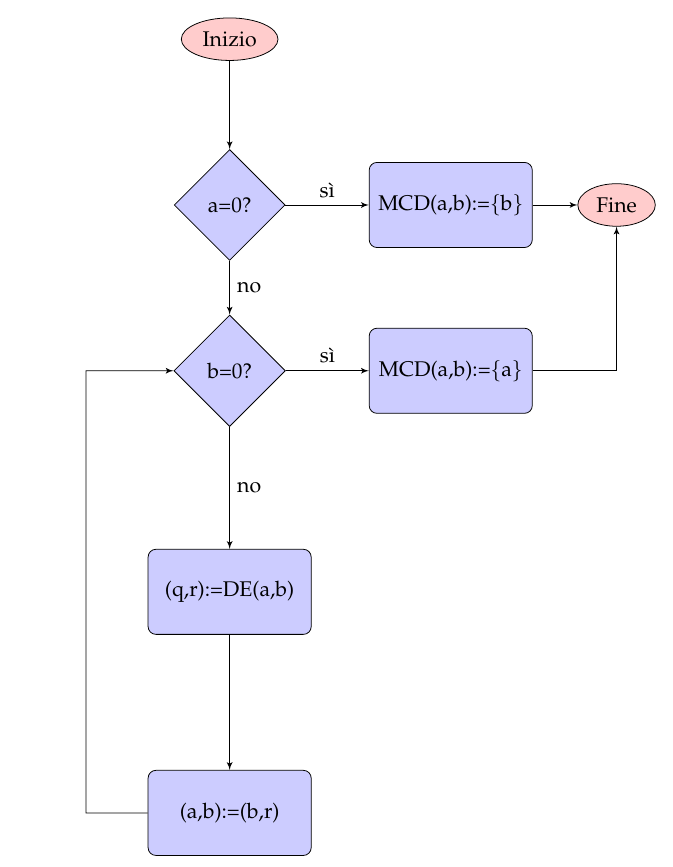
\includegraphics[scale=.55]{res/Algo_euclideo.png}
	\captionof{figure}{Algoritmo euclideo delle divisioni successive}
\end{center}

\subsection{Equazioni diofantee}\index{Equazione!Diofantea}

Oltre al calcolo dei massimi comun divisori, l’algoritmo euclideo permette di risolvere un altro importante problema.

\begin{defbox}{Equazione diofantea}
	Un’\textbf{equazione diofantea} è un’equazione in cui appaiano solo indeterminate e numeri interi che si intenda risolvere in $\mathbb{Z}$, cioè per la quale siano ammesse come soluzioni solo numeri interi.
\end{defbox} 

Ci occupiamo qui di un particolare tipo di equazione diofantea: quella cosiddetta lineare a due indeterminate, cioè una equazione diofantea della forma:
\begin{equation}\label{eq:diofantea}
	ax+by=c
\end{equation}

dove $a,b,c \in \mathbb{Z}$. Risolvere l'equazione \ref{eq:diofantea} significa trovare le coppie di interi $(u,v)$ tali che rendano vera l'uguaglianza se sostituiti a $x$ e $y$, cioè tali che $au+bv=c$. La \ref{eq:diofantea} può anche non ammettere soluzioni. Ad esempio, l'equazione $0x+0y=1$ non ammette ovviamente soluzioni. Facendo uso della terminologia introdotta sopra, è chiaro che \ref{eq:diofantea} ammette soluzioni (intere) se e solo se $c$ è combinazione lineare di $a$ e $b$ a coefficienti in $\mathbb{Z}$. Ciò permette di dimostrare la prima importante osservazione su questo genere
di equazioni.

\begin{teorbox}[di Bezout]\label{thm:bezout}\index{Bezout}
	Sono equivalenti le seguenti affermazioni:
	\begin{enumerate}
		\item Siano $a,b$ numeri interi relativi non nulli. Allora esiste un massimo comune divisore $d$ di $a$ e $b$ e risulta $d = au+bv$ per opportuni interi $u,v$.
		\item Siano $a,b \in \mathbb{Z}$ e sia $d = MCD(a,b)$. Allora l'insieme $\{\alpha a + \beta b \; | \; \alpha, \beta \in \mathbb{Z}\}$ delle combinazioni lineari di $a$ e $b$ a coefficienti in $\mathbb{Z}$ coincide con l'insieme $d\mathbb{Z}=\{dk \; | \; k \in \mathbb{Z}\}$ dei multipli di $d$ in $\mathbb{Z}$.
		\item Preso $d= MCD(a,b)$, l'equazione diofantea $ax+by=c$ ha soluzioni se e solo se $d \divides c$.
		\item Due numeri interi $a,b$ si dicono coprimi se e solo se 1 è combinazione lineare $a$ e $b$.
	\end{enumerate}
\end{teorbox}

\begin{proof}
\begin{enumerate}
	\item Ovvio, mediante l'algoritmo delle divisioni successive è possibile ricavare un'espressione di $d$ come combinazione lineare $au+bv$.
	\item Dal punto precedente sappiamo che $d=au+bv$. Quindi $d \in \{\alpha a + \beta b \; | \; \alpha, \beta \in \mathbb{Z}\}$. Moltiplicando $d$ per un qualunque $k \in \mathbb{Z}$ si ottiene quindi:
	\begin{align*}
		kd = a (\alpha k) + b (\beta k) \in \{\alpha a + \beta b \; | \; \alpha, \beta \in \mathbb{Z}\}
	\end{align*}
Quindi $d\mathbb{Z} \subseteq \{\alpha a + \beta b \; | \; \alpha, \beta \in \mathbb{Z}\}$. Analogamente abbiamo visto che una combinazione lineare di $a$ e $b$ è esprimibile come multiplo di $d$, quindi vale anche l'inclusione inversa e i due insiemi coincidono,
\item Supponiamo che l'equazione abbia soluzioni. Allora esistono $u,v \in \mathbb{Z}$ tali che $au+bv=c$, dunque $c$ è combinazione lineare di $a$ e $b$ a coefficienti in $\mathbb{Z}$, e quindi, per il punto precedente, è un multiplo di $d=MCD(a,b)$. Per definizione di multiplo ovviamente sappiamo che $d$ divide $c$. Dunque, se supponiamo che $d$ non divida $c$ dobbiamo trarre la conclusione che la nostra equazione non abbia soluzioni.
\item Non ha bisogno di dimostrazioni, è una definizione.
\end{enumerate}	
\end{proof}
\begin{lemmabox}[di Euclide]\index{Euclide}\label{lemma:euclide}
	Siano $a,b \in \mathbb{Z}$ coprimi. Se $c$ è un numero intero tale che $a \divides bc$ allora $a \divides c$.
\end{lemmabox}

\begin{proof}
	Per il teorema di Bezout esistono $u,v \in \mathbb{Z}$ tali che $1=au+bv$. D'altra parte $a$ divide $bc$ quindi $bc=ah$ per un opportuno numero intero $h$. Pertanto:
	\begin{align*}
		c &= c(au+bv) \\
		&= cau+cbv \\
		&= cau +ahv \\
		&= a(cu+hv)
	\end{align*}
	e quindi $a$ divide $c$.
\end{proof} 

\begin{example}
	Supponiamo di voler trovare soluzioni dell'equazione diofantea $74x+22y=10$. In questo caso è evidente che $MCD(74,22)=2$ e poiché $2 \divides 10$ siamo certi che l'equazione ammette soluzioni. Eseguendo le divisioni successive si ottiene:
	\begin{align*}
		74 &= 3 \cdot 22 + 8 \\
		22 &= 2 \cdot 8 + 6 \\
		8 &= 1 \cdot 6 + 2 \\
		6 &= 3 \cdot 2
	\end{align*}
	fino ad ottenere $2$ come ultimo resto non nullo. A questo punto possiamo esprimere i resti:
	\begin{align*}
		8 &= 74 - 3 \cdot 22 \\
		6 &= 22 - 2 \cdot 8 \\
		2 &= 8 - 1 \cdot 6
	\end{align*}
	e scrivere 2 come combinazione lineare di 74 e 22:
	\begin{align*}
		2 &= 8 - 6 & \\
		&= 8 - (22- 2 \cdot 8) & \text{\textcolor{gray}{(Sostituendo 6)}}\\
		&= 8 - 22 + 2 \cdot 8 \\
		&= 8 (1+2) - 22 &  \text{\textcolor{gray}{(Raccogliendo i coefficienti di 8)}}\\
		&= 3 \cdot 8 -22 \\
		&= 3 \cdot (74 - 3 \cdot 22) - 22 & \text{\textcolor{gray}{(Sostituendo 8)}} \\
		&= 3 \cdot 74 - 9 \cdot 22 - 22 \\
		&= 3 \cdot 74 - 10 \cdot 22 \\
		&= 3 \cdot 74 + (-10) \cdot 22
	\end{align*}
	Abbiamo così trovato che $2$ è esprimibile come combinazione lineare $\alpha 74 + \beta 22$ con $\alpha=3$ e $\beta=-10$. La coppia $(3,-10)$ è soluzione dell'equazione diofantea $74x+22y=2$. Moltiplicando per $5$ si ottiene $75 (15) + 22(-50) =10$, dunque la coppia $(15,-50)$ è la soluzione dell'equazione diofantea $74x+22y=10$.
\end{example}

\subsection{Struttura quoziente}\label{sez:congruenze}\index{Struttura!Quoziente}
Siano $S$ un insieme non vuoto, e $\bot: S \times S \longrightarrow S$ un'operazione in $S$.

\begin{defbox}{Compatibilità}
	Una relazione di equivalenza $\mathfrak{R} \in Eq(S)$ si dice \textbf{compatibile a sinistra} con $\bot$ se:
	\begin{displaymath}
		\forall x_{1},x_{2} \in S \Biggl((x_{1}\ \mathfrak{R} \ x_{2}) \implies \Bigl(\forall a \in S \bigl(a \bot x_{1} \ \mathfrak{R} \ a \bot x_{2}\bigr)\Bigr)\Biggr)
	\end{displaymath}
	Analogamente, $\mathfrak{R}$ si dice \textbf{compatibile a destra} con l'operazione $\bot$ se:
	\begin{displaymath}
		\forall x_{1},x_{2} \in S \Biggl((x_{1}\ \mathfrak{R} \ x_{2}) \implies \Bigl(\forall a \in S \bigl( x_{1} \bot a \ \mathfrak{R} \ x_{2} \bot a \bigr)\Bigr)\Biggr)
	\end{displaymath}
\end{defbox}

\begin{defbox}{Congruenza}\index{Congruenza}
	Sia $(S,\bot)$ una struttura algebrica. Una relazione di equivalenza $\mathfrak{R}$ in $S$ si dice una \textbf{congruenza} in $(S,\bot)$ se qualunque siano gli elementi $x_{1},x_{2},y_{1},y_{2}$ di $S$ tali che $x_{1} \ \mathfrak{R} \ x_{2}$ e $y_{1} \ \mathfrak{R} \ y_{2}$, risulta anche:
	\begin{displaymath}
		x_{1} \bot y_{1} \ \mathfrak{R} \ x_{2} \bot y_{2}
	\end{displaymath}
\end{defbox}


Pertanto, quando $\mathfrak{R}$ è una congruenza in $(S,\bot)$, e solo allora, è possibile considerare l'applicazione:
\begin{displaymath}
	\bot_{\mathfrak{R}}: ([x]_{\mathfrak{R}},[y]_{\mathfrak{R}}) \mapsto [x \bot y]_{\mathfrak{R}} \in S/{\mathfrak{R}}
\end{displaymath}
Tale applicazione è un'operazione nell'insieme quoziente $S/{\mathfrak{R}}$, chiamata \textbf{operazione quoziente} di $\bot$ rispetto a $\mathfrak{R}$. La struttura $(S/{\mathfrak{R}}, \bot_{\mathfrak{R}})$ viene chiamata \textbf{struttura quoziente}.


\begin{propbox}\label{prop:operazione_quoziente}
	Siano $S$ un insieme non vuoto, $\bot: S \times S \rightarrow S$ un'operazione in $S$ e $\mathfrak{R}$ una congruenza in $(S,\bot)$. Si ha:
	\begin{itemize}
		\item Se $\bot$ è associativa, allora anche $\bot_{\mathfrak{R}}$ è associativa;
		\item Se $\bot$ è commutativa, allora anche $\bot_{\mathfrak{R}}$ è commutativa;
		\item Se $u$ è un elemento neutro in $(S,\bot)$ allora $[u]_{\mathfrak{R}}$ è elemento neutro in $(S/{\mathfrak{R}},\bot_{\mathfrak{R}})$.
		\item Se $x$ è un elemento simmetrizzabile di $(S,\bot)$ e $x'$ è un suo simmetrico, allora $[x]_{\mathfrak{R}}$ è un elemento simmetrizzabile di $(S/{\mathfrak{R}},\bot_{\mathfrak{R}})$ e $[x']_{\mathfrak{R}}$ è un suo simmetrico.
	\end{itemize}
\end{propbox}

\begin{osservation}
	Una relazione di equivalenza $\mathfrak{R}$ è una congruenza in $(S,\bot_{1},\ldots,\bot_{n})$ se e soltanto se è compatibile con tutte le operazioni $\bot_{i}$ per ogni $i \in \{1, \ldots, n\}$.
\end{osservation}

\section{Congruenze in $\mathbb{Z}$}

\subsection{La relazione di congruenza modulo m}

Sia $m$ un numero intero relativo, e sia $\equiv_{m}$ la relazione binaria definita in $\mathbb{Z}$ ponendo:
\begin{equation}
	\forall a,b \in \mathbb{Z} \bigl(a \equiv_{m} b \iff m \divides (a-b)\bigr)
\end{equation}
ovvero se e solo se $a$ e $b$ sono numeri interi relativi tali che la differenza $(a-b)$ è multiplo di $m$, ovvero esiste $n \in \mathbb{Z}$ tale che $a-b=nm$.

Qualunque sia $a \in \mathbb{Z}$ risulta $a-a=0=0 \cdot m$, e quindi $a \equiv_{m} a$ e la relazione $\equiv_{m}$ risulta riflessiva. Siano $a,b$ numeri interi tali che $a \equiv_{m} b$. Allora risulta $a-b=km$ con $k \in \mathbb{Z}$, e quindi $b-a=-(a-b)=(-k)m$, sicché $b \equiv_{m} a$ e la relazione $\equiv_{m}$ è anche simmetrica. Siano infine $a,b,c$ numeri interi tali che $a \equiv_{m} b$ e $b \equiv_{m} c$. Allora esistono $h,k \in \mathbb{Z}$ tali che $a-b = km$ e $b-c=km$, sicché:
\begin{displaymath}
	a-c = (a-b)+(b-c) = hm+km=(h+k)m
\end{displaymath}
e quindi $a \equiv_{m} c$, e $\equiv_{m}$ è transitiva. Pertanto $\equiv_{m}$ \emph{è una relazione di equivalenza} in $\mathbb{Z}$. Se $a,b \in \mathbb{Z}$ sono due interi tali che $a \equiv_{m} b$ è possibile trovare usata la notazione $a \equiv b \ (mod. \ m)$.

Se $a$ è un numero intero relativo, la classe di equivalenza di $a$ rispetto alla relazione $\equiv_{m}$ si chiama ``\textbf{classe di congruenza} di $a$ modulo $m$'' e si denota col simbolo $[a]_{m}$. Un numero intero $b$ appartiene ad $[a]_{m}$ se e solo se $b \equiv_{m} a$, e quindi e se solo se $b-a=km$ per qualche $k \in \mathbb{Z}$. Pertanto:
\begin{displaymath}
	[a]_{m} = \{a +km \; | \; k \in \mathbb{Z}\}
\end{displaymath}
e in particolare:
\begin{displaymath}
	[0]_{m} = \{km \; | \; k \in \mathbb{Z}\} = m\mathbb{Z}
\end{displaymath}
dove $m\mathbb{Z}$ è l'insieme dei multipli di $m$. L'insieme quoziente $\mathbb{Z}/{\equiv_{m}}$ di $\mathbb{Z}$ rispetto alla relazione di equivalenza $\equiv_{m}$ si denota col simbolo $\mathbb{Z}_{m}$, e si chiama \textbf{insieme delle classi di interi modulo $m$}.

\begin{osservation}
	Poiché in $\mathbb{Z}$ l'unico multiplo di 0 è 0, si ha subito che la relazione $\equiv_{0}$ coincide con la relazione identica. D'altra parte ogni numero intero è divisibile per 1, sicché la relazione $\equiv_{1}$ è la relazione totale, e quindi $|\mathbb{Z}_{1}|=1$. È inoltre chiaro che per ogni intero relativo $m$ la relazione $\equiv_{m}$ e la relazione $\equiv_{-m}$ coincidono. Queste considerazioni consentono di limitare la nostra analisi al caso degli $m>1$.
\end{osservation}

\begin{example}
	Si consideri in $\mathbb{Z}$ la relazione di equivalenza $\equiv_{2}$. Due numeri interi $a,b \in \mathbb{Z}$ sono in relazione tra di loro se e solo se:
	\begin{displaymath}
		a \equiv_{2} b \iff 2 \divides (a-b) \iff \exists k \in \mathbb{Z} \bigl((a-b)=2k\bigr)
	\end{displaymath}
	ovvero se e soltanto se $(a-b)$ risulta un numero pari. Chiaramente la differenza tra due numeri interi è pari se e soltanto se $a$ e $b$ hanno la \textit{stessa parità} (entrambi pari oppure entrambi dispari). Infatti sia per assurdo $a$ un numero dispari e $b$ un numero pari della forma $2t$ per un opportuno $t \in \mathbb{Z}$. Essendo $a-b$ un numero pari esso sarà sicuramente della forma $2k$ per un qualche intero $k$.  Essendo $a$ un numero dispari questo può essere scritto nella forma $2n+1$ e si ha:
	\begin{displaymath}
		(a-b) = (2n+1)- 2t = 2n+1-2t= 2(n-t) + 1
	\end{displaymath}
	e $(a-b)$ risulterebbe un numero dispari, contro le nostre ipotesi.
\end{example}


\begin{example}
	Dati due numeri interi $x$ e $y$, diciamo che $x \equiv_{3} y$ se $(x-y)$ è multiplo di tre. Si vede subito che $0$ è congruo a tutti i multipli di tre. $1$ è congruo a tutti i numeri del tipo $\{\ldots, -5, -2, 1,4,7,10,\ldots\} = \{1+3k / k\in \mathbb{Z}\}$. $2$ è congruo a tutti i numeri del tipo $\{\ldots,-4,-1,2,5,8,11,\ldots\}=\{2+3k/k \in \mathbb{Z}\}$. Quindi nella partizione definita dalla congruenza modulo 3 ci sono tre classi di congruenza: $[0]_{3}, [1]_{3},[2]_{3}$.
\end{example}

\begin{propbox}
	Sia $m>1$ un numero intero. Qualunque sia il numero intero relativo $a$ risulta $a \equiv_{m} r$ dove $r$ è il resto della divisione euclidea di $a$ per $m$.
\end{propbox}

\begin{proof}
	Denotato con $q$ il quoziente della divisione euclidea di $a$ per $m$, si ha $a=mq+r$, con $0 \leq r < |m|$, per cui $(a-r) =mq$ e quindi $a \equiv_{m} r$.
\end{proof}


\begin{teorbox}
	Sia $m>1$ un numero intero. Allora $\mathbb{Z}_{m}$ è un insieme finito di ordine $m$ e risulta:
	\begin{displaymath}
		\mathbb{Z}_{m} = \{[0]_{m},[1]_{m},\ldots,[m-1]_{m}\}
	\end{displaymath}
\end{teorbox}


\begin{corolbox}
	Sia $m>1$ un numero intero, per ogni $a,b \in \mathbb{Z}$:
	\begin{displaymath}
		a \equiv_{m} b \iff \text{hanno lo stesso resto nella divisione euclidea per $m$}
	\end{displaymath}
\end{corolbox}

\begin{osservation}
	Si ha $m = 1 \cdot m + 0$ e quindi $m \equiv_{m} 0$. Ovvero $[m]_{m}=[0]_{m}$.
\end{osservation}

Per i risultati appena ottenuti possiamo vedere l'insieme quoziente $\mathbb{Z}_{m}$ come l'insieme delle \textbf{classi di resto modulo $m$}.


\begin{propbox}
	Le relazioni di congruenza sono compatibili con l'addizione. Dati i numeri interi $a,a',b,b' \in \mathbb{Z}$:
	\begin{equation}
	(a \equiv_{m} a' \land b \equiv_{m} b') \implies (a+b \equiv_{m} a'+b')
	\end{equation}
\end{propbox}

\begin{proof}
	Da $a \equiv_{m} a'$ e $b \equiv_{m} b'$ segue :
	\[
	\begin{cases}
		a-a' = km \\
		b-b' = hm
	\end{cases}
	\] per opportuni interi $h,k \in \mathbb{Z}$. Sommando membro a membro si ha:
	\begin{align*}
		a-a'+(b-b') = km+hm  \iff	a+b - (a'+b') = (h+k)m
	\end{align*}
	Quindi $a+b \equiv_{m} a'+b'$.
\end{proof}


\begin{propbox}
	Le relazioni di congruenza sono compatibili con la moltiplicazione. Dati i numeri interi $a,a',b,b' \in \mathbb{Z}$, vale:
	\begin{equation}
	(a \equiv_{m} a' \land b \equiv_{m} b') 	\implies	(a \cdot b \equiv_{m} a' \cdot b')
	\end{equation}
\end{propbox}

\begin{proof}
	È lasciata al lettore come esercizio.
\end{proof}

Da queste due proposizioni segue che:

\begin{teorbox}
	Qualunque sia il numero intero relativo $m$, la relazione di equivalenza $\equiv_{m}$ è una congruenza nella struttura algebrica $(\mathbb{Z},+,\cdot)$.
\end{teorbox}

È opportuno osservare che le uniche congruenze nella struttura algebrica $(\mathbb{Z},+,\cdot)$ sono le congruenze modulo $m$, al variare di $m \in \mathbb{Z}$. Questo teorema permette di introdurre nell'insieme $\mathbb{Z}_{m}$ delle classi di resto le operazioni quoziente dell'addizione e della moltiplicazione in $\mathbb{Z}$. Tali operazioni, denotate ancora con i simboli $+$ e $\cdot$, sono definite ponendo:
\begin{align*}
\begin{cases}
		[a]_{m}+[b]_{m} = [a+b]_{m}\\
	[a]_{m} \cdot [b]_{m} = [ab]_{m}
\end{cases}
\end{align*}
Tali operazioni sono associative e commutative, la classe $[0]_{m}$ è elemento neutro in $\mathbb{Z}_{m}$ rispetto all'addizione, mentre $[1]_{m}$ è elemento neutro rispetto alla moltiplicazione. Inoltre, per ogni numero intero relativo $a$, la classe $[a]_{m}$ è dotata di opposto in $\mathbb{Z}_{m}$ e risulta $-[a]_{m}=[-a]_{m}$. Infine, qualunque siano i numeri interi relativi $a,b,c \in \mathbb{Z}$ risulta:
\begin{align*}
	([a]_{m}+[b]_{m})[c]_{m} &=[a+b]_{m}[c]_{m} \\
	&=[(a+b)c]_{m}\\
	&=[ac+bc]_{m}\\
	&=[ac]_{m} + [bc]_{m}\\
	&=[a]_{m}[c]_{m} + [b]_{m}[c]_{m}
\end{align*}
sicché in $\mathbb{Z}_{m}$ la moltiplicazione è distributiva rispetto all'addizione. La struttura $(\mathbb{Z}_{m},+,\cdot)$ risulta quindi un anello.
Osserviamo che in $\mathbb{Z}_{m}$ non vale in generale la legge di annullamento del prodotto, ovvero esistono dei quozienti in cui sono presenti divisori dello zero.


\begin{example}
	Ad esempio in $\mathbb{Z}_{6}$ gli elementi $[2]_{6}$, $[3]_{6}$ e $[4]_{6}$ risultano essere divisori dello zero:
	\begin{align*}
		[2]_{6} \cdot [3]_{6} = [6]_{6} = [0]_{6} = [12]_{6}=[4]_{6} \cdot [3]_{6}
	\end{align*}
	e $\mathbb{Z}_{6}$ non risulta essere un anello integro, in particolare un dominio di integrità.
\end{example}


\begin{teorbox}
	Sia $m>1$ un numero intero relativo. Allora in $\mathbb{Z}_{m}$ vale la legge di annullamento del prodotto se e solo se $m$ è primo.
\end{teorbox}

\begin{propbox}\label{prop:invertibili_zm}
	Siano $a \in \mathbb{Z}$, $n \in \mathbb{N}^{*}$. $[a]_{m}$ è invertibile in $\mathbb{Z}_{m}$ se, e solo se, $a$ ed $m$ sono coprimi.
\end{propbox}

\begin{proof}Abbiamo:
\begin{itemize}
	\item[$\implies$] Se $[a]_{m}$ è invertibile, esiste $[b]_{m}$ tale che:
	\begin{displaymath}
		[a]_{m}\cdot[b]_{m} = [ab]_{m}=[1]_{m}
	\end{displaymath}
	Quindi: $$m \divides (1-ab) \iff \exists h \in \mathbb{Z} \bigl(1-ab = hm\bigr)$$ 
	Da $1=ab+hm$ e dal Teorema di Bezout segue che $a$ ed $m$ sono coprimi.
	
	\item[$\impliedby$] Viceversa, supposti $a$ ed $m$ coprimi tra di loro, essendo $(a,m)=1$ esistono $\alpha,\beta$ tali che $1=\alpha a + \beta m$. 
	
	Da $\alpha a-1 = -\beta m$ segue allora $\alpha a \equiv_{m} 1$ per cui $[\alpha a]_{m} = [\alpha]_{m} [a]_{m}$ e $[\alpha]_{m}$ è l'inverso di $[a]_{m}$.
\end{itemize}
\end{proof}


\begin{corolbox}
	Siano $a \in \mathbb{Z}$, $n \in \mathbb{N}^{*}$ e sia $[a]_{m} \neq [0]_{m}$. Allora $[a]_{m}$ è un divisore dello zero in $\mathbb{Z}_{m}$ se, e solo se, $a$ ed $m$ non sono coprimi.
\end{corolbox}

\begin{proof} Si ha:
	\begin{itemize}
		\item[$\implies$] Se $[a]_{m}$ è un divisore dello zero risulta non regolare e quindi non invertibile. Per la proposizione precedente allora $a$ ed $m$ non sono coprimi. 
		
		\item[$\impliedby$] Viceversa, se $d=(a,m)$ risulta $1<d<m$ ed esistono $a_{1},m_{1}$ tali che $a=a_{1}d$ ed $m=m_{1}d$. Dall'essere $1<n_{1}<n$ segue $[m_{1}]_{m} \neq [0]_{m}$ e $[a]_{m}[m_{1}]_{m} = [a_{1}dm_{1}]_{m} = [a_{1}]_{m}[m]_{m} = [a_{1}][0]_{m}= [0]_{m}$, per cui $[a]_{m}$ è un divisore dello zero.
	\end{itemize}
\end{proof}

\begin{corolbox}
	Siano $a \in \mathbb{Z}$ ed $m \in \mathbb{N}^{*}$ sia $[a]_{m} \neq [0]_{m}$. Allora $[a]_{m}$ è invertibile se e solo se non è un divisore dello 0.
\end{corolbox}

\begin{teorbox}[Caratterizzazione anello degli interi modulo $m$]\label{thm:car_anelli_zm}
	Sia $m>1$ un intero. Allora le seguenti affermazioni sono equivalenti:
	\begin{enumerate}
		\item l'anello $\mathbb{Z}_{m}$ è un campo;
		\item L'anello $\mathbb{Z}_{m}$ è un dominio di integrità;
		\item $m$ è un numero primo.
	\end{enumerate}
\end{teorbox}

\begin{proof}
	Le condizioni $(1)$ e $(2)$ sono equivalenti per il Corollario precedente. Per dimostrare l'equivalenza di $(1)$ e $(3)$ si osservi che, se $m$ è primo, tutti gli interi $1, \ldots, m-1$ sono coprimi con $m$ e quindi tutte le classi $[1]_{m},[2]_{m},\ldots [m-1]_{m}$ sono invertibili. Viceversa, supposto che $\mathbb{Z}_{m}$ sia un campo, se $m$ non fosse primo esisterebbe un divisore $m_{1}$ di $m$ tale che $1 < m_{1} < m$. Allora risulterebbe $[m_{1}]_{m} \neq [0]_{m}$ ed $[m_{1}]_{m}$ non invertibile, essendo $(m,m_{1}) = m_{1}>1$. Dall'assurdo segue che $m$ è necessariamente primo.
\end{proof} 


\begin{corolbox}
	Gli elementi non nulli di $\mathbb{Z}_{m}$ sono tutti invertibili se e solo se $m$ è primo.
\end{corolbox}

\subsubsection{Periodo di un elemento}\index{Periodo}
Il concetto di classe di resto ha a che fare con la nozione di periodo di un elemento in un gruppo. Ricordiamo che, se un gruppo $G$ è denotato con la notazione additiva, allora il concetto di potenza coincide con il concetto di multiplo. Quindi si dice che $G$ è ciclico se esiste $a \in G$ tale che $G=\langle a \rangle = \{na / n \in \mathbb{Z}\}$.

\begin{lemmabox}
	Sia $G=\langle x \rangle$ un gruppo ciclico. Allora $G$ è finito se e solo se esiste un numero intero positivo $m$ tale che $x^{m}=1$.
\end{lemmabox}

\begin{proof}
	Se $G$ è finito, esistono dei numeri interi positivi $h$ e $k$ tali che $x^{h}=x^{k}$. Supposto, per fissare le idee, $h>k$, si ha $m=h-k>0$ e $x^{m}=x^{h-k}=x^{h}(x^{k})^{-1}=1$. Reciprocamente, esista un numero intero positivo $m$ tale che $x^{m}=1$. Qualunque sia il numero intero relativo $n$, si ha per il teorema della divisione euclidea: $n=mq+r$, con $q$ ed $r$ numeri interi relativi tali che $0\leq r < m$. Allora $x^{n}= x^{mq+r}=(x^{m})^{q}x^{r}=x^{r}$. Per cui $G=\{x^{0},x^{1},\ldots,x^{m-1}\}$ è finito.
\end{proof}


\begin{teorbox}[Teorema ponte]
	Sia $G=\langle x \rangle$ un gruppo ciclico finito di ordine $m$. Allora $G=\{x^{0},x^{1},\ldots,x^{m-1}\}$ ed $m$ è minimo intero positivo tale che $x^{m}=1$.
\end{teorbox}

\begin{defbox}{Elemento periodico}\index{Elemento!Periodico}
	Sia $G$ un gruppo. Un elemento $x \in G$ si dice \textbf{periodico} se il sottogruppo $\langle x \rangle$ è finito. In questo caso l'ordine di $\langle x \rangle$ si chiama \textbf{periodo} di $x$ e si denota con il simbolo $o(x)$. Un gruppo $G$ si dice \textbf{periodico} se ogni suo elemento è periodico.
\end{defbox}

\begin{osservation}
	Un elemento $x$ di $G$ è periodico se e solo se esiste $m \in \mathbb{Z}$ tale che $x^{m}=1_{G}$ se $G$ è denotato moltiplicativamente. Nel caso in cui $G$ è denotato additivamente allora $x \in G$ è periodico se $mx = 0_{G}$.
\end{osservation}

\begin{lemmabox}
	Sia $(G,\cdot)$ un gruppo e $x \in G$ un elemento periodico di periodo $n$. Allora:
	\begin{displaymath}
		\forall a \in \mathbb{Z} \bigl(x^{a} = x^{rest(a,n)}\bigr)
	\end{displaymath}
	dove $rest(a,n)$ è il resto della divisione euclidea di $a$ per $n$.
\end{lemmabox}
\begin{proof}
	Sia $r=rest(a,n)$ allora esiste un $k \in \mathbb{Z}$ tale che $a=kn+r$. Allora:
	\begin{align*}
		x^{a} &= x^{kn+r}\\
		&= (x^{n})^{k} \cdot x^{r}\\
		&= 1_{G}  \cdot x^{r} = x^{r}
	\end{align*}
	e l'asserto è dimostrato.
\end{proof}

\begin{propbox}
	Sia $(G,\cdot)$ un gruppo e $x \in G$ un elemento periodico di periodo $n$. Allora:
	\begin{displaymath}
		\forall a,b \in \mathbb{Z} \bigl(x^{a} = x^{b} \iff a \equiv_{n} b \iff rest(a,n) = rest(b,n)\bigr)
	\end{displaymath}
\end{propbox}
\begin{proof}
\begin{itemize}
		\item[$\impliedby$] Se $a \equiv_{m} b$ allora $m \divides (a-b)$. Ovvero $(a-b)= q m$ per un opportuno $q \in \mathbb{Z}$. Allora $a= q m+ b$ e risulta:
	\begin{displaymath}
		x^{a} = x^{qm +b} = (x^{m})^{q} \cdot x^{b} = (1_{G}) \cdot x^{b} = x^{b}
	\end{displaymath}
	\item[$\implies$] Se $x^{a} = x^{b}$ allora $x^{a-b}=1_{G} = x^{0}$ e quindi vale $a \equiv_{m} b$.
\end{itemize}
\end{proof}

\begin{defbox}{Funzione di Eulero}\index{Funzione di Eulero}
	La funzione $\varphi$ di Eulero è l'applicazione di $\mathbb{N}^{*}$ in sè definita ponendo, per ogni $n \in \mathbb{N}^{*}$:
	\begin{equation}
		\varphi(n)=|\{a \in \mathbb{N}^{*} \; | \; a \leq n \land MCD(a,n)=1 \}|
	\end{equation}
	ovvero il numeri degli interi positivi minori di $n$ e primi con $n$.
	
\end{defbox}

\begin{example}
	Ad esempio, poiché tra gli interi positivi $1,2,3,4,5,6$ ad essere coprimi con $6$ sono solo $1$ e $5$ si ha $\varphi(6)=2$.
\end{example}

La funzione di Eulero esprime la cardinalità del gruppo degli invertibili dei quozienti di $\mathbb{Z}$. Infatti, per ogni $n \in \mathbb{N}^{*}$, sappiamo che gli elementi dell'anello $\mathbb{Z}_{n}$ corrispondono precisamente ai numeri interi positivi tali che $a \leq n$, nel senso che:
\begin{displaymath}
	\mathbb{Z}_{n} = \{[a]_{n} \; | \; a \in \mathbb{N}^{*} \land a \leq n \}
\end{displaymath}

e se $a$ e $b$ sono interi positivi minori o uguali a $n$ si ha $[a]_{n} = [b]_{n}$ se e solo se $a=b$. Sappiamo inoltre che, con queste stesse notazioni, $[a]_{n}$ è invertibile in $\mathbb{Z}_{n}$ se e solo se $a$ ed $n$ sono coprimi. Dunque:

\begin{displaymath}
	\mathcal{U}(\mathbb{Z}_{n}) = \{[a]_{n} \; | \; a \in \mathbb{N}^{*} \land a \leq n \land MCD(a,n) = 1\}
\end{displaymath}
ovvero:

\begin{displaymath}
	|\mathcal{U}(\mathbb{Z}_{n})|=\varphi(n)
\end{displaymath}

\begin{example}
	Il gruppo composto dall'insieme finito $\mathbb{Z}_{4}=\{[0]_{4},[1]_{4},[2]_{4},[3]_{4}\}$ insieme all'operazione di addizione è un gruppo ciclico in quanto esiste un elemento generatore in grado di generare tutti gli elementi di $\mathbb{Z}_{4}$. Infatti, preso $[1]_{4}$ si ha:
	\begin{displaymath}
		\begin{array}{l}
			([1]_{4})^{1} = 1 \cdot [1]_{4} =[1 \cdot 1]_{4} = [1]_{4}\\
			([1]_{4})^{2} = 2 \cdot [1]_{4} =[2 \cdot 1]_{4} = [2]_{4}\\
			([1]_{4})^{3} = 3 \cdot [1]_{4} =[3 \cdot 1]_{4} = [3]_{4}\\
			([1]_{4})^{4} = 4 \cdot [1]_{4} =[4 \cdot 1]_{4} = [4]_{4} = [0]_{4}\\
		\end{array}
	\end{displaymath}
	Il periodo dell'elemento $[1]_{4}$ è uguale a quattro, infatti, il sottogruppo generato da $[1]_{4}$, ovvero l'insieme $\langle [1]_{4} \rangle = \{n [1]_{4} / n \in \mathbb{Z}\} = \{[0]_{4},[1]_{4},[2]_{4},[3]_{4}\}$ coincide con l'insieme $\mathbb{Z}_{4}$. L'elemento $[2]_{4}$ non è un generatore perché i suoi multipli (potenze) non generano tutti gli altri elementi dell'insieme $\mathbb{Z}_{4}$:
	\begin{displaymath}
		\langle [2]_{4} \rangle = \{[0]_{4},[2]_{4}\}
	\end{displaymath}
	Il periodo dell'elemento $[2]_{4}$ è 2 perché il numero intero più piccolo $k$ tale che $2^{k} = 0_{\mathbb{Z}_{4}}$ è $k=2$. Infatti:
	\begin{displaymath}
		([2]_{4})^{2} = [2]_{4}+[2]_{4} = [4]_{4} = [0]_{4}
	\end{displaymath}
	Anche l'elemento $[3]_{4}$ è un generatore del gruppo ciclico in quanto il sottogruppo $\langle [3]_{4} \rangle $ coincide con $\mathbb{Z}_{4}$:
	\begin{displaymath}
		\langle [3]_{4} \rangle = \{[0]_{1},[2]_{4},[3]_{4}\}
	\end{displaymath}
	Il periodo di $[3]_{4}$ risulta quindi uguale a quattro perché sono necessarie quattro ripetizioni dell'operazione per avere l'elemento neutro $([3]_{4})^{4}=[0]_{4}$. Quindi $\mathbb{Z}_{4}$ ha due generatori ($[1]_{4}$ e $[3]_{4}$) e vale:
	\begin{displaymath}
		\langle [1]_{4} \rangle = \langle [3]_{4} \rangle = \mathbb{Z}_{4}
	\end{displaymath}
	notiamo inoltre che $1$ e $3$ sono coprimi con $4$ e vale $\varphi(4)=2$. Infatti, il numero di generatori distinti di un gruppo ciclico di ordine $m$ coincide con il numero di interi positivi strettamente minori di $m$ e coprimi con $m$, ovvero $\varphi(m)$.
\end{example}

A conclusione di questa trattazione sulle proprietà dei gruppi ciclici vogliamo mostrare che, a meno di isomorfismi, \emph{gli unici gruppi ciclici finiti}, ovvero i gruppi per i quali esiste un elemento $x$ tale che $x^{m}=1$, \emph{sono i gruppi additivi} $(\mathbb{Z}_{m},+)$. Infatti, considerato un gruppo ciclico finito $G$ e l'applicazione $f: n \in \mathbb{Z} \rightarrow x^{n} \in G$, poiché $G=\{x^{n} / n \in \mathbb{Z}\}$ si ha che $f$ è suriettiva. Qualunque siano gli elementi $m,n \in \mathbb{Z}$ si ha inoltre:
\begin{displaymath}
	f(m+n)= x^{m+n}=x^{m}+x^{n}=f(m)+f(n)
\end{displaymath}
ed $f$ risulta essere un epimorfismo. Dal Teorema di omomorfismo segue allora che $G$ è isomorfo a $\mathbb{Z}/{\mathfrak{R}_{f}}$ dove $\mathfrak{R}_{f}$ è nucleo di equivalenza di $f$. Se $|G|=m$ si ha $\mathfrak{R}_{f}$ è equivalente\footnote{Si tenga sempre a mente che $f$ è una applicazione che associa ogni intero $n$ alla potenza $x^{n} \in G$. Se $G$ è un gruppo ciclico denotato additivamente allora $f$ è definita ponendo $n \mapsto nx$.} a $\equiv_{m}$ e $G$ è isomorfo a $\mathbb{Z}_{m}$.

\begin{corolbox}
	L'anello $(\mathbb{Z}_{m},+,\cdot)$ ha caratteristica pari ad $m$.
\end{corolbox}
\begin{proof}
	Per ogni $a \in \mathbb{Z}$:
	\begin{displaymath}
		[a]_{m} = [0]_{m} \iff a \equiv_{m} 0 \iff m \divides (a-0) \iff m \divides a \iff a =km
	\end{displaymath}
	ed $m$ risulta essere la caratteristica dell'anello $\mathbb{Z}_{m}$.
\end{proof}

\subsection{Equazioni congruenziali}\index{Equazioni!Congruenziali}
Nel paragrafo precedente è stata data una condizione necessaria e sufficiente affinché una classe $[a]_{m} \neq [0]_{m}$ sia invertibile. In questa sezione si vedrà come è possibile determinare $[a]_{m}^{-1}$ quando $[a]_{m}$ è invertibile\footnote{Ovvero quando $a$ ed $m$ sono coprimi.}.

Si ricordi che un elemento $[a]_{m}$ è invertibile in $\mathbb{Z}_{m}$ quando esiste $[c]_{m} \in \mathbb{Z}_{m}$ tale che: $[a]_{m}[c]_{m}=[ac]_{m}=[1]_{m}$ ovvero se esiste $c \in \mathbb{Z}$ tale che $ac \equiv_{m} 1$. In generale vale la seguente definizione:

\begin{defbox}{Equazioni congruenziali}
	Siano $a,b,m \in \mathbb{Z}$ e sia $m>1$. L'espressione	$ax \equiv_{m} b$ si dice \textbf{equazione congruenziale} di termini $a$ e $b$ modulo $m$. Un numero intero relativo $c$ si dice \textbf{soluzione} dell'equazione congruenziale $ax \equiv_{m} b$ se risulta $ac \equiv_{m} b$. Ciò equivale a richiedere che sia $[a]_{m}[c]_{m} = [b]_{m}$.
\end{defbox}

\begin{osservation}
	Un elemento $[a]_{m} \in \mathbb{Z}_{m}$ è invertibile se, e solo se, l'equazione congruenziale $ax \equiv_{m} 1$ ammette una soluzione.
\end{osservation}

\begin{propbox}[Criterio di compatibilità]
	Siano $a,b, m \in \mathbb{N}^{*}$, $d=MCD(a,m)$. L'equazione congruenziale $ax \equiv_{m} b$ ha soluzione se, e solo se, $d$ divide $b$.
\end{propbox}

\begin{proof}Dimostriamo le due implicazioni:
\begin{itemize} 
	\item[$\implies$] Se $c$ è una soluzione dell'equazione congruenziale allora $\exists k \in \mathbb{Z}$ tale che $ac-b=km$. Allora da $d \divides a$ e $d \divides m$ segue $d \divides ac-km = b$.
	
	\item[$\impliedby$] Viceversa, si supponga $d$ divisore di $b$: esiste $h \in \mathbb{Z}$ tale che $b=dh$. Essendo inoltre $d$ un massimo comune divisore tra $a$ ed $m$, esistono degli interi $r$ ed $s$ tali che $d=ra+sm$. Da ciò segue $b=hd=h(ra+sm)$. In particolare, da $hra-b=-hsm$ segue che $hr$ è una soluzione dell'equazione congruenziale.
\end{itemize}
\end{proof}

\begin{propbox}
	Siano $a,b \in \mathbb{Z}$, $m \in \mathbb{N}^{*}$, $t$ un divisore comune di $a,b,m$. Allora le soluzioni dell'equazione congruenziale $ax \equiv_{m} b$ sono tutte e sole quelle dell'equazione congruenziale:
	\begin{displaymath}
		\frac{a}{t} x \equiv_{\frac{m}{t}} \frac{b}{t}
	\end{displaymath}
\end{propbox}

\begin{proof}
	È sufficiente osservare che, se $c$ è un intero, allora:
	\begin{align*}
		m &= t \cdot \frac{m}{t} \divides ac-b = t \cdot \frac{a}{t} \cdot c-t \cdot \frac{b}{t} \iff \frac{m}{t} \divides \frac{a}{t} \cdot c -\frac{b}{t}
	\end{align*}
\end{proof}

\begin{corolbox}
	Una congruenza compatibile $ax \equiv_{m} b$ ammette esattamente $d = MCD(a,m)$ soluzioni \textit{non congruenti} modulo $m$ date da:
	\begin{equation}
		x_{0} + k \frac{m}{d}
	\end{equation}
	dove $x_{0}$ è una soluzione della congruenza e $0 \leq k < d$.
\end{corolbox}

\begin{osservation}
	Se $MCD(a,m)=1$ allora la congruenza lineare ha un'unica soluzione.
\end{osservation}

\begin{propbox}
	Sia $c$ una soluzione dell'equazione congruenziale $ax \equiv_{m} 1$. Allora, se $b$ è un intero, $cb$ è soluzione dell'equazione congruenziale $ax \equiv_{m} b$.
\end{propbox}

\begin{proof}
	Basta osservare che, se $m$ divide $ac-1$, divide anche $(ac-1)b =acb-b$.
\end{proof}

\begin{propbox}
	Si consideri l'equazione congruenziale $ax \equiv_{m} b$ e siano $a$ ed $m$ primi tra loro. Allora l'equazione ha soluzioni, che costituiscono una classe di resto modulo $m$.
\end{propbox}

\begin{proof}
	Poiché $1=MCD(a,m)$ divide $b$ l'equazione ha soluzioni. Indicata con $c$ una di tali soluzioni, verifichiamo che l'insieme $X$ di tutte e sole le soluzioni dell'equazione coincide con $[c]_{m}$. Sia $y \in X$ una soluzione, da $ac \equiv_{m} b$ e $ay \equiv_{m} b$ segue:
	\begin{displaymath}
		ac \equiv_{m} ay \implies m \divides ac-ay = a (c-y)
	\end{displaymath}
	Ciò implica, essendo inoltre $m$ ed $a$ primi tra loro, che $m$ divide $c-y$, per cui $y \in [c]_{m}$. Viceversa, se $y \in [c]_{m}$, risulta $[c]_{m}=[y]_{m}$ e quindi $[a]_{m}[y]_{m}=[a]_{m}[c]_{m}=[b]_{m}$ come si voleva.
\end{proof}

\gbox{Tecniche di semplificazione}{red}{
	Data l'equazione congruenziale:
\begin{equation}\label{eq:congruenziale}
	ax \equiv_{m} c
\end{equation} dove $a,c,m \in \mathbb{Z}$ e $m \neq 0$:
\begin{enumerate}
	\item Se $a' \in [a]_{m}$ e $c' \in [c]_{m}$, l'equazione congruenziale $$a'x \equiv_{m} c'$$ è equivalente alla \ref{eq:congruenziale}.
	\item Per ogni $k \in \mathbb{Z}$, se $k \neq 0$, l'equazione congruenziale $$akx \equiv_{mk} ck$$ è equivalente alla \ref{eq:congruenziale}.
	\item Per ogni $t \in \mathbb{Z}$, se $t$ è coprimo con $m$, l'equazione congruenziale $$atx \equiv_{m} ct$$ è equivalente a \ref{eq:congruenziale}.
\end{enumerate}
}
\subsubsection{Esempi di equazioni congruenziali e loro soluzioni}
\begin{example}
	L'equazione $324x \equiv_{508} 127$ non ha soluzioni in quanto $MCD(324,508) \ndivides 127$.
\end{example}
\begin{example}
	L'equazione $120x \equiv_{m} 128$ ha soluzioni (4 è MCD tra 120 e 164 e divide 128). Troviamole. 
	
	Dividiamo tutto per 4: l'equazione diventa $30x \equiv_{41} 32$ che risulta essere una equazione congruenziale ridotta ai minimi termini in quanto 30 e 41 risultano essere coprimi. Eseguiamo l'algoritmo euclideo per risolvere l'equazione diofantea $1 = 30x + 41y$ si ottiene:
	\begin{align*}
		41 &= (1)30 + 11 \\
		30 &= (2)11 + 8 \\
		11 &=(1)8 + 3 \\
		8 &= (2)3+2 \\
		3 &=(1)2 +1 \\
		2 &=(2)1 +0
	\end{align*} 
Ricaviamo quindi le seguenti relazioni:
\begin{align*}
	11&=(1)41+(-1)30 \\
	8&=(1)30+(-2)11 \\
	3&=(1)11+(-1)8 \\
	2&=(1)8+(-2)3 \\
	1&=(1)3+(-1)2
\end{align*}
Dalle quali possiamo eseguire il seguente calcolo per ottenere una combinazione lineare di 30 e 41 che dia 1 come risultato:
\begin{align*}
	1 &= (1)3 +(-1)2 \\
	&=(1)3+(-1)\bigl(8+(-2)3\bigr)\\
	&= (-1)8 + (3)3 \\
	&=(-1)8 +(3)\bigl(11+(-1)8\bigr)\\
	&=(3)11 +(-4)8 \\
	&=(3)11+(-4)\bigl(30+(-2)11\bigr)\\
	&=(-4)30 + (11)11 \\
	&=(-4)30 + (11)\bigl(41 +(-1)30\bigr)\\
	&=(11)41 +(-15)30
\end{align*}
Pertanto, $1=(11 )\cdot 41 + (-15)\cdot 30$. Più significativamente: abbiamo scoperto che vale $(-15)30 \equiv_{41}  1$, cioè che l'inverso di $[30]_{41}$ in $\mathbb{Z}_{41}$ è $[-15]_{41}$. A questo punto sappiamo che l'unica classe in $\mathbb{Z}_{41}$ che, moltiplicata per $[30]_{41}$ dia $[32]_{41}$ è $([30]_{41})^{-1}[32]_{41}=[-15]_{41}[32]_{41} = [(-15)(32)]_{41}$. Questa classe è l'insieme delle soluzioni, in $\mathbb{Z}$, dell'equazione congruenziale originaria.
\end{example}

\begin{example}
	L'equazione $4x \equiv_{10} 8$ ha ovviamente 2 come soluzione in $\mathbb{Z}$. L’insieme di tutte le soluzioni non è $[2]_10$ ma $[2]_5$, perché in
	forma ridotta l’equazione diventa $2x \equiv_{5} 4$, notare: 2 e 5 sono coprimi. Si può osservare che, ad esempio, $7 \in [2]_{5} \setminus [2]_{10}$, quindi $[2]_{5}$ è strettamente contenuto in $[2]_{10}$; è facile anche verificare che $[2]_{5}$ è l’unione disgiunta di $[2]_{10}$ e $[7]_{10}$, quindi, l’equazione data, vista come equazione in $Z_{10}$: $[4]_{10} X = [8]_{10}$ ha esattamente due soluzioni: $[2]_{10}$ e $[7]_{10}$.
\end{example}

\begin{example}
	L’equazione $45x \equiv_{47} 476$ si risolve immediatamente senza bisogno di calcoli: evidentemente $45 \equiv_{47} -2$ e $476 \equiv_{47} 6$, quindi l’equazione è equivalente a (nel senso che ha le stesse soluzioni di) $-2x \equiv_{47} 6$, ovvero (dividendo -2 e 6 per -2, che è invertibile modulo 47) a $x \equiv_{47} -3$, che è già risolta: l’insieme delle soluzioni è $[-3]_{47}$.
\end{example}

\begin{example}
	L’equazione $32x - 4 \equiv_{18} 8$ non è altro che un modo diverso di scrivere $32x \equiv_{18} 12$. Per semplificarla possiamo dividere tutto per 2 (MCD tra 32 e 18), ottenendo $16x \equiv_{9} 6$. Da questa, siccome 2 è coprimo con 9, quindi invertibile modulo 9, dividendo 16 e 6 per 2 ricaviamo l’equazione equivalente $8x \equiv_{9} 3$; ma $8 \equiv_{9} -1$, quindi possiamo
	riscrivere questa come $-x \equiv_{9} 3$, ovvero $x \equiv_{9} -3$, e l’equazione originaria è risolta. In alternativa: da $32x \equiv_{18} 12$
	passiamo a $-4x \equiv_{18} 12$, perché $-4 \equiv_{18} 32$, quindi, dividendo tutto per 2, a $-2x \equiv_{9} 6$; possiamo ancora dividere -2
	per 2, o direttamente per -2, perché, di nuovo, 2 e -2 sono invertibili modulo 9, per ottenere ancora $x \equiv_{9} -3$ e così l’insieme $[-3]_{9}$ di tutte le soluzioni.
\end{example}


\begin{example}
	\begin{enumerate}
	\item Un esempio simile: $14x \equiv_{111} 21$ ha le stesse soluzioni di $2x \equiv_{111} 3$; qui bisogna fare attenzione al fatto che
	7, per il quale abbiamo diviso 14 e 21, e 111 sono coprimi. Come facciamo a saperlo? Be’, $111 \equiv_{7} 111 - 70 = 40$,
	siccome 42 è multiplo di 7 certamente non lo è 40 (infatti $40 \equiv_{7} -2$), quindi 7 non divide 111; poiché 7 è primo questo garantisce che 7 e 111 sono coprimi. A questo punto dobbiamo risolvere $2x \equiv_{111} 3$. Possiamo farlo usando l’algoritmo euclideo, oppure osservando che, siccome 3 è dispari come 111, allora $3 + 111$ è pari, ne ricaviamo l’intero $(3 + 111)/2 = 114/2 = 57$, allora $2 \cdot 57 = 3 + 111 \equiv_{57} 3$ e così vediamo che 57 è soluzione dell'equazione. Dal momento che l’equazione è ridotta (2 e 111 sono coprimi), l’insieme delle soluzioni è $[57]_{111}$.

	\item Si consideri l'equazione congruenziale:
	\begin{equation}
		ax \equiv_{m} b
	\end{equation}
	\paragraph{Caso A:} \textit{Risoluzione dell'equazione congruenziale del tipo:} $ax \equiv_{m} 1$ con $MCD(a,m)=1$.
	
	Essendo $1=MCD(a,m)$ è possibile determinare, mediante l'algoritmo di Euclide delle divisioni successive, degli interi $\alpha$ e $\beta$ tali che risulti $\alpha a + \beta m = 1$. L'intero $\alpha$ risulta essere una soluzione dell'equazione e $[\alpha]_{m}$ coincide con l'insieme delle soluzioni dell'equazione.
	
	\paragraph{Caso B:} \textit{Risoluzione della generica equazione congruenziale} $ax \equiv_{m} b$.
	
	\begin{enumerate}
		\item Verificare che $d=MCD(a,m)$ divida $b$; infatti, questa è condizione necessaria affinché l'equazione ammetta soluzioni. Se $d$ divide $b$ si può continuare;
		\item Posto $\overline{a} = \frac{a}{d}$, $\overline{b}=\frac{b}{d}$ e $\overline{m}=\frac{m}{d}$, si considera l'equazione $$\overline{a}x \equiv_{\overline{m}} \overline{b}$$ che ammette tutte e sole le soluzioni dell'equazione originale ed è tale che $MCD(\overline{a},\overline{m})=1$.
		\item Determinare una soluzione $c$ dell'equazione congruenziale $\overline{a}x \equiv_{\overline{m}} 1$ mediante il metodo illustrato nel Caso A.
	\end{enumerate}
	
	\item Si dica se l'equazione congruenziale $20x \equiv_{34} 4$ ammette soluzioni; in caso di risposta affermativa, determinare l'insieme di tutte le soluzioni.
	
	\paragraph{Risoluzione}
	\begin{enumerate}
		\item Si calcola il massimo comun divisore tra $20$ e $34$. In tal caso si ha $MCD(20,34)=2$ ed, essendo $2 \divides 4$, si ha che l'equazione ammette soluzioni che coincidono con quelle dell'equazione $10x \equiv_{17} 2$.
		\item Si studia l'equazione $10x \equiv_{17} 1$. Mediante l'algoritmo di Euclide si determinano gli interi $h,k$ tali che $1=10h+17k$. In questo caso $h=-5$ e $k=3$. Quindi:
		\begin{align*}
			1 = (3)17 +(-5)10 \implies 2 = (6)17 + (-10)10
		\end{align*}
	Quindi $[-10]_{17}$ è soluzione dell'equazione $10x \equiv_{17} 2$. Chiaramente $[-10]_{17}=[7]_{17}$.
	\end{enumerate}
\end{enumerate}
\end{example}

\section{L'anello dei polinomi}

\subsection{Definizione e terminologia essenziale}

\begin{defbox}{Polinomio}
	Sia $A$ un anello commutativo unitario ed indichiamo con $0$ l'elemento neutro in $A$ rispetto all'operazione di addizione. Una funzione $f : \mathbb{N} \rightarrow A$ si dice \textbf{successione di elementi di $A$} e si denota con $(a_{n})_{n \in \mathbb{N}}$.
	\bigskip
	
	Una successione $(a_{n})_{n \in \mathbb{N}}$ di elementi di $A$ si dice \textbf{polinomio a coefficienti in $A$} se è \emph{definitivamente nulla}, ovvero se:
	\begin{equation}
		\exists k \in \mathbb{N} \bigl( (\forall n \geq k) (a_{n}=0)\bigr)
	\end{equation}
	L'insieme di tutti i polinomi a coefficienti in $A$ si denota con il simbolo $A[x]$.
\end{defbox}

\begin{example}
	Sia $f:\mathbb{N} \rightarrow A$ la successione che associa ogni numero naturale all'elemento neutro in $A$. Chiaramente tale successione è un polinomio definitivamente nullo in quanto per ogni $n \geq 0$ si ha $a_{n}=0$. Tale polinomio prende il nome di \textbf{polinomio nullo} ed è denotato anche col simbolo $0_{A}$.
\end{example}


\begin{defbox}{Grado di un polinomio}
	Se $f \in A[x] \setminus \{0_{A}\}$ e $(a_{i})_{i \in \mathbb{N}}$ è la successione dei coefficienti di $f$ allora l'insieme $S_{f} = \{i \in \mathbb{N} \; | \; a_{i} \neq 0_{A} \}$ è finito e quindi, essendo un sottoinsieme finito non vuoto di $\mathbb{N}$, ha massimo; questo massimo è chiamato \textbf{grado} del polinomio $f$, denotato col simbolo $deg(f)$ (o anche con altri simboli, tra i quali $deg (f)$, $deg \ f$ e $\delta(f)$).
\end{defbox}

\begin{defbox}{Coefficiente direttore e polinomi monici}
	Il coefficiente $a_{deg(f)}$ di posto $deg(f)$ si chiama \textbf{coefficiente direttore} di $f$ e si indica con $cd (f)$. Un polinomio $f$ è detto \textbf{monico} se e solo se il suo coefficiente direttore è $1_{A}$. Il coefficiente di posto $i=0$ viene invece chiamato \textbf{termine noto}.
\end{defbox}


\begin{osservation}
	In $(\mathbb{Z},+,\cdot)$ consideriamo la successione: $\{a_{1}=0;\; a_{2}=3;\; a_{4}=0, \; a_{5}=1, \; a_{6}= 0, \ldots \forall n \geq 6 (a_{n}=0)\}$. Tale successione risulta essere una successione di elementi di $\mathbb{Z}$ definitivamente nulla in quanto esiste $k \in \mathbb{Z}$ ($k=6$)per il quale ogni $n \geq k$ i termini $a_{n}$ sono nulli. Il grado di tale polinomio può essere visto anche come:
	\begin{displaymath}
		min_{k \in \mathbb{N}} \{k \in \mathbb{N} \; | \; (\forall n \geq k) (a_{n}=0)\}
	\end{displaymath}
	ovvero il minimo indice $k$ per il quale la successione è definitivamente nulla. Quindi $deg(f)=5$ mentre $a_{deg(f)}=1$. Il polinomio ha grado 5 ed in particolare è monico in quanto il suo coefficiente direttore è pari a 1.

	Il polinomio nullo risulta avere coefficiente direttore pari a $0_{A}$ mentre, per convenzione, si pone $deg(0_{A})=-\infty$ per indicare il fatto che il grado del polinomio nullo è il più piccolo di ogni altro polinomio.
\end{osservation}

Due polinomi $(a_{n})_{n \in \mathbb{N}}$ e $(b_{n})_{n \in \mathbb{N}}$ sono
\textit{uguali} se $a_{n} = b_{n}$ per ogni $n \in \mathbb{N}$. All'interno di $A[x]$ possiamo considerare le operazioni:
\begin{eqnarray}
	+: \bigl((a_{n})_{n \in \mathbb{N}},(b_{n})_{n \in \mathbb{N}}\bigr) \in A[x] \times A[x] \mapsto (a_{n}+b_{n})_{n \in \mathbb{N}}\\
	\cdot:\bigl((a_{n})_{n \in \mathbb{N}},(b_{n})_{n \in \mathbb{N}}\bigr) \in A[x] \times A[x] \mapsto \Bigl(\sum_{i+j=n} a_{i} \cdot b_{j}\Bigr)_{n \in \mathbb{N}}
\end{eqnarray}


\begin{example}
	Sia $A= \mathbb{Z}$ e si considerino i polinomi $a_{n}=\{1, 2, 0, \ldots\}$ e $b_{n}=\{2,0,\ldots\}$. Si ha:
	\begin{displaymath}
		a_{n} + b_{n} = \{1+2, 2+0, \ldots\} = \{3,2,0, \ldots\}
	\end{displaymath}
	mentre il prodotto:
	\begin{align*}
		a_{n} \cdot b_{n} = \{ a_{0}b_{0} &=1 \cdot 2 = 2, \\
		a_{0}b_{1}+a_{1}b_{0}&=0+4 = 4,\\
		a_{1}b_{1}+a_{0}b_{2}+a_{2}b_{0} &= 0\} = \{2,4,0,\ldots\}
	\end{align*}
\end{example}

\begin{propbox}
	La struttura $(A[x],+,\cdot)$ è un anello commutativo con unità il polinomio $(1,0,0,\ldots)$.
\end{propbox}

\begin{proof}
	Chiaramente l'operazione di addizione risulta commutativa ed associativa e $(A[x],+)$ risulta un semigruppo commutativo. Inoltre, poiché $A$ risulta un anello, per ogni elemento $a \in A$ esiste l'opposto rispetto all'operazione di somma ed è dunque possibile definire la successione opposta $(-a_{n})_{n \in \mathbb{N}}$ e $(A[x],+)$ risulta quindi un gruppo abeliano.
	
	L'elemento neutro rispetto all'operazione di addizione è il polinomio nullo $0_{A}$ e l'elemento neutro rispetto all'operazione di moltiplicazione è il polinomio costante $1_{A}$. Inoltre, l'operazione di moltiplicazione risulta commutativa e associativa e $(A[x],\cdot)$ risulta un semigruppo commutativo. Infine, l'operazione di moltiplicazione risulta distributiva rispetto all'operazione di addizione e $(A[x],+,\cdot)$ risulta un anello commutativo con unità.
\end{proof}

\begin{defbox}{Polinomio costante}
	Sia $(a_{n})_{n \in \mathbb{N}}$ un polinomio a coefficienti in $A$. Tale polinomio si dice \textbf{costante} se e solo se per ogni $n \in \mathbb{N}^{*}$ risulta $a_{n}=0_{A}$. In tal caso il polinomio costante si denota con il simbolo $a_{0}$. Un polinomio è costante se:
	\begin{displaymath}
		\exists a \in A \bigl( (a_{n})_{n \in \mathbb{N}} = (a,0,0,\ldots) \bigr)
	\end{displaymath}
\end{defbox}

\begin{osservation}
	Il polinomio nullo è un polinomio costante.
\end{osservation}

Consideriamo l'applicazione: $ \varphi: a \in A \mapsto (a,0,\ldots) \in A[x]$.
\begin{propbox}
	$\varphi$ è un omomorfismo tra gli anelli $(A,+,\cdot)$ e $(A[x],+,\cdot)$. In particolare $\varphi$ è un monomorfismo.
\end{propbox}

\begin{proof}
	Per ogni $a,b \in A$ si ha:
	\begin{align*}
		\varphi(a+b) &= (a+b,0,0,\ldots) \\
		&= (a,0,0,\ldots)+(b,0,0,0) & \text{\textcolor{gray}{Per la definizione di somma in $A[x]$}}\\
		&= \varphi(a) + \varphi(b)
	\end{align*}
	Analogamente, per ogni $a,b \in A$:
	\begin{align*}
		\varphi(a \cdot b) &= (ab,0,0,\ldots) \\
		&= (a,0,0,0,\ldots) \cdot (b,0,0,0,\ldots) & \text{\textcolor{gray}{Per la definizione di prodotto in $A[x]$}}\\
		&= \varphi(a) \cdot \varphi(b)
	\end{align*}
	Dimostriamo ora che $\varphi$ è iniettiva. Per ogni $a,b \in A$:
	\begin{align*}
		\varphi(a)= \varphi(b) &\iff (a,0,0,0,\ldots) = (b,0,0,0,\ldots) \iff a=b
	\end{align*}
	E l'asserto è dimostrato.
\end{proof}

Per il teorema di omomorfismo, $A$ è isomorfo all'insieme $im(\varphi)=\{(a,0,0,\ldots) \; | \; a \in A \} $. Identifichiamo quindi $A$ con l'insieme dei polinomi costanti ed è lecito definire ogni elemento $a \in A$ come il polinomio costante che ha per termine noto il termine $a$.

Poniamo $x=(0,1,0,\ldots)$ e consideriamo il prodotto $x^{2}$:
\begin{align*}
	x^{2} &= x \cdot x \\
	&= (0,1,0,0,\ldots) \cdot (0,1,0,0,\ldots)\\
	&= (0,0,1,0,\ldots) & \text{\textcolor{gray}{Applicando la definizione di prodotto}}
\end{align*}
Supponendo che: $$x^{n-1}= (\underbrace{0,\ldots,0}_{\text{$n-1$ zeri}},1,0,\ldots)$$ si dimostra per induzione che:
\begin{align*}
	x^{n} &= x^{n-1}\cdot x\\
	&= (0,\ldots,0,1,0,\ldots) \cdot (0,1,0,\ldots)\\
	&= (\underbrace{0,\ldots,0}_{\text{$n$ zeri}},1,0,0,\ldots)
\end{align*}
Allora quando consideriamo $ax^{n}$ si ottiene:
\begin{align*}
	(a,0,0,\ldots)\cdot (\underbrace{0,\ldots,0}_{\text{$n$ zeri}},1,0,0,\ldots) &= (\underbrace{0,\ldots,0}_{\text{$n$ zeri}},a,0,\ldots)
\end{align*}
Supposto $f \in A[x]$ di grado $m$, ovvero:
\begin{displaymath}
	f= (a_{0},a_{1},\ldots,a_{m},0,\ldots)
\end{displaymath}
allora $f$, per come abbiamo definito la somma e per quanto appena visto per i polinomi del tipo $ax^{n}$, si può scrivere come:
\begin{equation}\label{eq:polinomio}
	f = a_{0} + a_{1}x + a_{2}x^{2}+\ldots+a_{m}x^{m}
\end{equation}
che risulta la classica rappresentazione dei polinomi.

\subsection{Proprietà universale}
La proprietà più importante degli anelli di polinomi è la seguente:

\begin{propbox}[Proprietà universale per anelli di polinomi ad una indeterminata]
	Sia $A[x]$ un anello di polinomi nell’indeterminata $x$ sull’anello commutativo unitario $A$. Si fissino un anello commutativo unitario $B$ ed un omomorfismo: $\theta: A \longrightarrow B$ di anelli unitari e $b \in B$. Allora esiste uno ed un solo omomorfismo: $\theta^{*}: A[x] \longrightarrow B$ di anelli unitari tale che $\theta^{*}(x)=b$ e $\theta$ sia la restrizione di $\theta^{*}$ ad $A$.
\end{propbox}

In altre parole, fissato un omomorfismo $\theta: A \rightarrow B$, esiste ed è unico l'omomorfismo:
\begin{equation}
	\theta^{*} : \sum_{i=0}^{n} a_{i}x^{i} \in A[x] \mapsto \sum_{i=0}^{n}\theta(a_{i})b^{i} \in B
\end{equation}

che rende commutativo il diagramma a sinistra (l'omomorfismo $A \hookrightarrow A[x]$ è l'immersione di $A$ in $A[x]$) come mostrato nel diagramma a destra:
\begin{center}
	\begin{minipage}{.45\textwidth}
		\centering
		\begin{tikzpicture}
			\node[name=A]{$A$};
			\node[name=B,right=3cm of A]{$B$};
			\node[name=ax,below=.5cm of A,xshift=1.5cm]{$A[x]$};
			\draw[->] (A)--node[above,midway]{$\theta$}(B);
			\draw[right hook-stealth](A)--(ax);
		\end{tikzpicture}
	\end{minipage}
	\hfil
	\begin{minipage}{.45\textwidth}
		\centering
		\begin{tikzpicture}
			\node[name=A]{$A$};
			\node[name=B,right=3cm of A]{$B$};
			\node[name=ax,below=.5cm of A,xshift=1.5cm]{$A[x]$};
			\draw[->] (A)--node[above,midway]{$\theta$}(B);
			\draw[right hook-stealth](A)--(ax);
			\draw[dashed,->](ax)to node[below,midway]{$x \stackrel{\theta^{*}}{\mapsto} b$}(B);
		\end{tikzpicture}
	\end{minipage}
\end{center}

Vediamo alcune importanti applicazioni della proprietà universale:
\begin{itemize}
	\item \textit{Unicità dell'anello dei polinomi, a meno di isomorfismi.} Supponiamo che $A[x]$ e $A[y]$ siano due anelli di polinomi ad una indeterminata sullo stesso anello (commutativo unitario) $A$, con indeterminate, rispettivamente $x$ e $y$. Applichiamo la proprietà universale scegliendo come $\theta$ l'immersione $A \hookrightarrow A[y]$ e, come $b$, l'elemento $y$. Otteniamo così un unico omomorfismo $\alpha: A[x] \rightarrow A[y]$ tale che $\alpha(x) = y$ e la restrizione di $\alpha$ ad $A$ sia l'immersione, cioè $\alpha(a)=a$ per ogni $a \in A$. Poiché anche $A[y]$ è un anello di polinomi, possiamo ripetere la stessa costruzione scambiando i ruoli di $A[x]$ e $A[y]$.
	\begin{center}
		\begin{minipage}{.45\textwidth}
			\centering
			\begin{tikzpicture}
				\node[name=A]{$A$};
				\node[name=B,right=3cm of A]{$A[y]$};
				\node[name=ax,below=.5cm of A,xshift=1.5cm]{$A[x]$};
				\draw[right hook-stealth] (A)--(B);
				\draw[right hook-stealth](A)--(ax);
				\draw[->](ax)to node[below,midway]{$x \stackrel{\alpha}{\mapsto} b$}(B);
			\end{tikzpicture}
		\end{minipage}
		\hfil
		\begin{minipage}{.45\textwidth}
			\centering
			\begin{tikzpicture}
				\node[name=A]{$A$};
				\node[name=B,right=3cm of A]{$A[x]$};
				\node[name=ax,below=.5cm of A,xshift=1.5cm]{$A[y]$};
				\draw[right hook-stealth] (A)--(B);
				\draw[right hook-stealth](A)--(ax);
				\draw[->](ax)to node[below,midway]{$x \stackrel{\beta}{\mapsto} b$}(B);
			\end{tikzpicture}
		\end{minipage}
	\end{center}
	
	Ottenendo un omomorfismo $\beta: A[y] \rightarrow A[x]$ tale che $\beta(y)=x$ e $\beta(a)=a$ per ogni $a \in A$. È facile verificare che $\alpha$ e $\beta$ sono l'uno l'inverso dell'altro. Infatti, per ogni elemento $f= \sum_{i=0}^{n} a_{i}x^{i}$ di $A[x]$ si ha: $$\beta(\alpha(f))=\beta(\sum_{i=0}^{n}a_{i}y^{i})=\sum_{i=0}^{n}a_{i}x^{i}=f$$ e, similmente: $$\alpha(\beta(g))= \alpha(\sum_{i=0}^{n}b_{i}x^{i})=\sum_{i=0}^{n}b_{i}y^{i} = g$$ per ogni $g \in A[y]$. Ciò prova che $\alpha$ è un isomorfismo.
	
	Dunque, assegnati due anelli di polinomi ad una indeterminata su A esiste un isomorfismo tra questi due anelli di polinomi che manda l’indeterminata del primo nell’indeterminata del secondo e manda in se stesso ogni elemento di $A$. Con le notazioni appena usate, questo isomorfismo è l’applicazione:
	\begin{displaymath}
		\alpha: \sum_{i=0}^{n} a_{i}x^{i} \in A[x] \mapsto \sum_{i=0}^{n} a_{i}y^{i} \in A[y]
	\end{displaymath}
	osserviamo esplicitamente che essa manda ogni polinomio $f$ di $A[x]$ nel polinomio di $A[y]$ che ha la stessa successione dei coefficienti di $f$. Possiamo dunque dire, in modo un poco approssimativo ma efficace, che due anelli di polinomi sullo stesso anello commutativo unitario $A$ possono solo differire per il nome dell’indeterminata; in questo senso, a meno di isomorfismi, ne esiste solo uno.
	
	\item \textit{Omomorfismo di sostituzione.} L’applicazione più frequente della proprietà universale si ha per il caso in cui $B = A$ e $\theta$ è l’applicazione
	identica di $A$. In questo caso la proprietà ci dice che per ogni $c \in A$ esiste uno ed un solo omomorfismo di anelli unitari $A[x] \rightarrow A$ che manda ogni elemento di $A$ in sé e $x$ in $c$:
	\begin{center}
		\begin{tikzpicture}
			\node[name=A]{$A$};
			\node[name=B,right=3cm of A]{$A$};
			\node[name=ax,below=.5cm of A,xshift=1.5cm]{$A[x]$};
			\draw[->] (A)--node[above,midway]{$id_{A}$}(B);
			\draw[right hook-stealth](A)--(ax);
			\draw[->](ax)to node[below,midway,yshift=-5pt]{$x \mapsto c$}(B);
		\end{tikzpicture}
	\end{center}
	È facile descrivere esplicitamente questo omomorfismo. Per ogni $f  = \sum_{i=0}^{n} a_{i}x^{i} \in A[x]$ poniamo $f(c) = \sum_{i=0}^{n} a_{i}c^{i}$. L'omomorfismo di cui stiamo parlando è allora l'applicazione:
	\begin{displaymath}
		f \in A[x] \mapsto f(c) \in A
	\end{displaymath}
	che chiamiamo \textbf{omomorfismo di sostituzione}.
	
	\item Per ogni intero positivo $m$, sia $\epsilon_{m} : n \in \mathbb{Z} \mapsto [n]_{m} \in \mathbb{Z}$, la proiezione canonica $\mathbb{Z} \twoheadrightarrow \mathbb{Z}_{m}$ (il simbolo di freccia a doppia punta ci ricorda il fatto che $\epsilon_{m}$ è un omomorfismo suriettivo). Componendo questa con l'immersione $\iota_{m}: \mathbb{Z}_{m} \hookrightarrow \mathbb{Z}_{m}[x]$ otteniamo l'omomorfismo di anelli unitari $\iota_{m} \circ \epsilon_{m} = \epsilon_{m}\iota_{m} : n \in \mathbb{Z} \mapsto [n]_{m} \in \mathbb{Z}_{m}[x]$. La proprietà universale fornisce l'omomorfismo $\overline{\epsilon_{m}}$ qui descritto:
	
	\begin{center}
		\begin{tikzpicture}
			\node[name=A]{$\mathbb{Z}$};
			\node[name=B,right=3cm of A]{$\mathbb{Z}_{m}$};
			\node[name=C,right=3cm of B]{$\mathbb{Z}_{m}[x]$};
			\node[name=ax,below=1cm of A,xshift=3cm]{$\mathbb{Z}[x]$};
			\draw[->_>] (A)to node[above,midway]{$\epsilon_{m}$}(B);
			\draw[right hook-stealth](B)--node[above,midway]{$\iota_{m}$}(C);
			\draw[right hook-stealth](A)--(ax);
			\draw[->_>](ax)to node[below,midway,yshift=-5pt]{$x \stackrel{\overline{\epsilon_{m}}}{\mapsto}x$}(C);
		\end{tikzpicture}
	\end{center}
	
	Più esplicitamente, l'immagine mediante $\overline{\epsilon_{m}}$ di $f = \sum_{i=0}^{n} a_{i}x^{i} \in \mathbb{Z}[x]$ è il polinomio $f_{m} = \sum_{i=0}^{n}[a_{i}]_{m}x^{i}$. $f_{m}$ è detto \textbf{polinomio $f$ riguardato come polinomio a coefficienti in $\mathbb{Z}_{m}$}.
\end{itemize}

\subsection{Grado di somme e prodotto di polinomi}
Siano, ancora, $A$ un anello commutativo unitario, e siano $f,g \in A[x]$, con successioni dei coefficienti, rispettivamente, $(a_{n})_{n \in \mathbb{N}}$ e $(b_{n})_{n \in \mathbb{N}}$. Supponiamo anche $f \neq 0_{A} \neq g$ e poniamo $n= deg(f)$, $m= deg(g)$. Grazie alla notazione introdotta (Formula \ref{eq:polinomio} ) possiamo ridefinire le operazioni di addizione e moltiplicazione di polinomi in $A[x]$.

\begin{propbox}
	Siano  $f,g \in A[x]$ e sia $m= deg(f)$ ed $n = deg(g)$. Allora, posto $M=max\{m,n\}$ si ha:
	\begin{eqnarray}
		f+g &= \sum_{i=0}^{M} (a_{i}+b_{i})x^{i}\\
		f \cdot g &= \sum_{i=0}^{m+n}\bigl(\sum_{j=0}^{i}a_{j}\cdot b_{i-j}\bigr)x^{i}
	\end{eqnarray}
\end{propbox}

\begin{proof}
	Consideriamo la somma $f+g$:
	\begin{align*}
		f+g &= (a_{0}+a_{1}x+\ldots+a_{m}x^{m})+(b_{0}+b_{1}x+\ldots+b_{n}x^{n})\\
		&= a_{0}+b_{0}+a_{1}x+b_{1}x+\ldots+a_{M}x^{M}+b_{M}x^{M} \\
		&= a_{0}+b_{0}+(a_{1}+b_{1})x+\ldots+(a_{M}+b_{M})x^{M} & \text{\textcolor{gray}{Applicando la distributività di $\cdot$ rispetto a $+$}}\\
		&= \sum_{i=0}^{M} (a_{i}+b_{i})x^{i}
	\end{align*}
	Per quanto riguarda il prodotto, invece:
	\begin{align*}
		f \cdot g &= (a_{0}+a_{1}x+\ldots+a_{m}x^{m}) \cdot (b_{0}+b_{1}x+\ldots+b_{n}x^{n})\\
		&= a_{0} \cdot (b_{0}+b_{1}x+\ldots+b_{n}x^{n}) + a_{1}x \cdot (b_{0}+b_{1}x+\ldots+b_{n}x^{n}) + \ldots a_{m}x^{m}\cdot (b_{0}+b_{1}x+\ldots+b_{n}x^{n}) \\
		&= a_{0}b_{0} + a_{0}b_{1}x + \ldots + a_{0}b_{n}x^{m} + a_{1}b_{0}x + a_{1}b_{1}x^{2}+\ldots+ a_{m}b_{0}x^{m}+ \ldots + a_{m}b_{1}x^{m+1}+ \ldots + a_{m}b_{n} x^{m+n} \\
		&= a_{0}b_{0} +(a_{0}b_{1}+a_{1}b_{0})x+(b_{0}a_{2}+a_{0}b_{2}+a_{1}b_{1})x^{2} + \ldots + (a_{m}b_{n})x^{m+n} \\
		&= \sum_{i=0}^{m+n}\bigl(\sum_{j=0}^{i}a_{j}\cdot b_{i-j}\bigr)x^{i}
	\end{align*}
	Come volevasi dimostrare.
\end{proof}

Cosa possiamo dire sul grado di questi tre polinomi? Consideriamo in primo luogo il polinomio $f+g$. Nella sua espressione non compaiono potenze di $x$ con esponente superiore ad $M$, quindi certamente $deg(f+g)\leq M$, e $deg(f+g)=M$ se, e solo se, il coefficiente di posto $M$ in $f+g$ (cioè $a_{M}+b_{M}$) è diverso da zero. Distinguiamo tre casi:
\begin{enumerate}
	\item Se $n<m$ allora $M=m$ e $a_{m}=0_{A}$, quindi $a_{M}+b_{M}=b_{M} \neq 0_{A}$. In questo caso, dunque, $deg (f+g)=m=M$. Inoltre $cd(f+g)=b_{m}=cd(g)$.
	\item Similmente, se $n>m$, vediamo che $f+g$ ha grado $n$ e coefficiente direttore $a_{n}=cd(f)$.
	\item Se $n=m$ bisogna fare una distinzione ulteriore: 
	\begin{enumerate}
		\item Se $a_{n}+b_{n}\neq 0_{A}$ abbiamo $deg(f+g) = n = M$ e $cd (f+g) = a_{n}+b_{n}$
		\item Se $a_{n}+b_{n} = 0_{A}$ (cioè $a_{n}=-b_{n}$) allora certamente $deg(f+g)<n$
	\end{enumerate}
\end{enumerate}


\begin{propbox}
	Se $A$ è un anello commutativo unitario e $f,g \in A[x] \setminus 0_{A}$, allora:
	\begin{equation}
		deg(f+g)=max \{deg(f),deg(g)\}
	\end{equation}
	a meno che $deg(f)=deg(g)$ e $cd(f)=-cd(g)$. In questo secondo caso:
	\begin{equation}
		deg(f+g)<deg(f)=deg(g)
	\end{equation}
\end{propbox}


\begin{propbox}
	Se $A$ è un anello commutativo unitario e $f,g \in A[x] \setminus \{0_{A}\}$, allora:
	\begin{equation}
		deg(f-g) = max\{deg(f),deg(g)\}
	\end{equation}
	a meno che $deg(f)=deg(g)$ e $cd(f)=cd(g)$. In questo secondo caso:
	\begin{equation}
		deg(f-g)<deg(f)=deg(g)
	\end{equation}
\end{propbox}


\begin{example}
	Se $f=3x^{2}+x+1$ e $g=2x^{2}+x+2$ sono polinomi a coefficienti interi (con $deg(f)=deg(g)=2$) allora:
	\begin{displaymath}
		f-g=x^{2}-1
	\end{displaymath}
	ha anch'esso grado due. Se invece $g=3x^{2}+x+2$ allora $deg(f)=deg(g)$ e $cd(f)=cd(g)$ e quindi:
	\begin{displaymath}
		f-g=-1
	\end{displaymath}
	ha grado zero.
\end{example}

Passiamo ora a considerare il grado di $fg$. Il ragionamento è simile: poiché nell'espressione di $fg$ non appaiono potenze di $x$ con esponente superiore a $n+m$ certamente $deg(fg)\leq n+m$ e vale $deg(fg) = n+m$ se, e solo se, $a_{n}b_{n} \neq 0$.


\begin{propbox}
	Se $A$ è un anello commutativo unitario e $f,g \in A[x] \setminus \{0_{A}\}$, posto $a=cd(f)$ e $b=cd(g)$ si ha:
	\begin{eqnarray}
		ab \neq 0_{A} &\implies& cd(fg)=ab \land deg(fg)=deg(f)+deg(g) \label{eq:regola_add_gradi}\\
		ab = 0_{A} &\implies& deg(fg)<deg(f)+deg(g)
	\end{eqnarray}
\end{propbox}


Se vale la \ref{eq:regola_add_gradi} si dice che per i polinomi $f$ e $g$ vale la \textbf{regola di addizione dei gradi}. Ovviamente questa regola vale sempre nel caso in cui uno dei due polinomi sia il polinomio nullo. Alcune importanti conseguenze di tale regola sono le seguenti:


\begin{corolbox}
	Sia $A$ un anello commutativo unitario e sia $f \in A[x]$. Se $cd(f)$ è cancellabile in $A$ allora $f$ è cancellabile in $A[x]$ e, per ogni $g \in A[x]$, si ha $deg(fg)=deg(f) +deg(g)$.
\end{corolbox}


\begin{proof}
	Sia $g \in A[x]\setminus \{0_{A}\}$ e siano $a=cd(f)$ e $b=cd(g)$. Poiché $a$ è cancellabile in $A$, quindi non un divisore dello zero, e $b \neq 0_{A}$ allora $ab \neq 0_{A}$. Per quanto osservationervato in precedenza vale allora la \ref{eq:regola_add_gradi} e sicuramente $fg \neq 0_{A}$. Quindi $f$ non è un divisore dello zero e quindi è cancellabile.
\end{proof}


\begin{propbox}
	Sia $A$ un anello commutativo unitario. Sono equivalenti:
	\begin{enumerate}
		\item $A$ è un dominio di integrità;
		\item Per ogni coppia di polinomi in $A[x]$ vale la regola di addizione dei gradi;
		\item $A[x]$ è un dominio di integrità.
	\end{enumerate}
	Inoltre, se $A$ è un dominio di integrità allora $\mathcal{U}(A[x])=\mathcal{U}(A)$.
\end{propbox}


\begin{proof}
	$(1) \implies (2)$ Per ogni polinomio $f \in A[x]$ distinguiamo due casi:
	\begin{enumerate}
		\item $f\neq 0_{A}$: allora $cd(f)$ è non nullo e quindi cancellabile in $A$ in quanto dominio di integrità ed è possibile applicare il Corollario precedente.
		\item Se $f=0_{A}$ vale sempre la regola di addizione dei gradi.
	\end{enumerate}
	
	Ovviamente $(2) \implies (3)$ in quanto se vale la regola di addizione dei gradi allora $\forall f,g  \in A[x] (fg \neq 0_{A})$ e allora vale la legge di annullamento del prodotto in $A[x]$ che quindi risulta un dominio di integrità.
	
	$(3) \implies (1)$ banale: se $A[x]$ è un dominio di integrità e $a,b \in A \setminus \{0_{A}\}$ allora $ab \neq 0_{A}$ perché altrimenti $a$ sarebbe un divisore dello zero in $A[x]$.
	
	Resta da provare solo che $\mathcal{U}(A[x])= \mathcal{U}(A)$ se valgono le condizioni $(1)$, $(2)$ e $(3)$.
	
	Se $a \in \mathcal{U}(A)$ e $b$ è l'inverso di $a$ in $A$, allora $ab = 1_{A} = 1_{A[x]}$, quindi $b$ è anche l'inverso di $a$ in $A[x]$, dunque $a \in \mathcal{U}(A[x])$. Pertanto $\mathcal{U}(A)\subseteq \mathcal{U}(A[x])$.
	
	Nell'ipotesi che $A$ sia un dominio di integrità sia, viceversa, $f \in \mathcal{U}(A[x])$ e sia $g$ l'inverso di $f$ in $A[x]$. Allora $fg=1_{A}$ e, ovviamente, $f \neq 0_{A} \neq g$. Poiché in $A[x]$ vale la regola di addizione dei gradi, $deg(f) + deg(g) = deg(fg)=deg(1_{A})=0_{A}$. Dunque, $deg(f)$ e $deg(g)$ sono due numeri naturali la cui somma è $0$; di conseguenza $deg(f) = deg(g) = 0$. Ciò mostra che $f \in A$ e $g \in A$, quindi sia $f$ che il suo inverso sono elementi di $A$, dunque $f \in \mathcal{U}(A)$.
	
	Abbiamo così provato anche l'inclusione inversa. 
\end{proof}


\begin{example}
	Vediamo così che la regola di addizione dei gradi non vale per polinomi su anelli che non siano domini di integrità, ed è importante osservare che per tali anelli può non valere neanche la conclusione finale dell'ultima proposizione appena dimostrata: non è detto che i polinomi invertibili siano costanti. Consideriamo l'anello $A=(\mathbb{Z}_{4},+,\cdot)$ e il polinomio di grado 1 a coefficienti in $A$:
	\begin{displaymath}
		f= [1]_{4} + [2]_{4}x
	\end{displaymath}
	Calcolando il prodotto $f \cdot f$ si ottiene:
	\begin{align*}
		f \cdot f &= ([1]_{4} + [2]_{4}x) \cdot ([1]_{4} + [2]_{4}x) \\
		&= [1]_{4} +[2]_{4}x+[2]_{4}x +[4]_{4}x \\
		&= [1]_{4} + [8]_{4}x \\
		&= [1]_{4}
	\end{align*}
	Ottenendo così un polinomio costante (di grado zero). In particolare osserviamo che $f$ risulta invertibile e coincide con il proprio inverso. In questo caso notiamo che non vale la regola di addizione dei gradi in quanto, ricordando il Teorema di caratterizzazione dell'anello degli interi modulo $m$ (Teorema \ref{thm:car_anelli_zm}), $\mathbb{Z}_{4}$ non risulta essere un dominio di integrità in quanto $4$ non è primo. Notiamo infatti che il coefficiente direttore di $f$, $[2]_{4}$, è un divisore dello zero.
	
\end{example}

\begin{propbox}[Condizione di non invertibilità]
	Sia $f \in A[x]$. Se $f$ è cancellabile e $deg(f)>0$, allora $f$ non è invertibile.
	
\end{propbox}

\begin{proof}
	Per assurdo, sia $f$ invertibile e sia $g=f^{-1}$ un suo inverso. Allora per la \ref{eq:regola_add_gradi}:
	\[deg(f)+deg(g)=deg(fg)=deg(1)=0 \implies deg(f)=0\]
	il che è assurdo. 
\end{proof}


\begin{example}
	\textit{I polinomi monici di grado maggiore di zero non sono mai invertibili}. Qualunque sia l'anello commutativo unitario non nullo $A$, l'indeterminata $x$ non è mai invertibile in $A[x]$. Infatti, se $x$ fosse invertibile, detto $g$ il suo inverso, avremmo $1_{A} = xg$ e quindi $deg(xg)=0$ ma, valendo la \ref{eq:regola_add_gradi}, si ha $def(xg)=deg(x)+deg(g)=1+deg(g)$, in contraddizione con quanto appena detto. Di conseguenza, \textit{qualsiasi sia l'anello commutativo unitario non nullo} $A$, in $A[x]$ esistono elementi non invertibili e diversi dallo zero, quindi $A[x]$ \textit{non è un campo}.
\end{example}


\subsection{Divisione con resto tra polinomi}
Se $f$ e $g$ sono due polinomi su un anello commutativo unitario $A$, con $g \neq 0_{A}$, diciamo che in $A[x]$ è possibile effettuare la divisione di $f$ (il \textit{dividendo}) per $g$ (il \textit{divisore}) se e solo se esistono $q,r \in A[x]$ tali che $f=gq+r$ e $deg (r) < deg(g)$. Un'osservazione banale è che se, nella situazione appena descritta, $deg(f) < deg(g)$ allora è sicuramente possibile effettuare la divisione di $f$ per $g$: basta porre $q = 0$ e $r=f$.



\begin{teorbox}[della divisione lunga]
	Siano $A$ un anello commutativo e $f,g \in A[x]$. Supponiamo che $cd(g) \in \mathcal{U}(A)$. Allora esiste una ed una sola coppia $(q,r) \in A[x] \times A[x]$ tale che $f=gq+r$ e $deg(r) < deg(g)$.
\end{teorbox}

\begin{proof}
	Iniziamo a provare l'esistenza di $(q,r)$. Come appena osservato, se $deg(f) < deg(g)$ una coppia con le proprietà richieste si ottiene ponendo $q=0$ e $r=f$. Possiamo allora supporre $n = deg(f)$,  $m = deg(g)$ e sia $n\geq m$. osserviamo che l'ipotesi su $cd(g)$ garantisce che $cd(g) \neq 0_{A}$ e quindi $n,m \in \mathbb{N}$. 
	
	Ragioniamo per induzione su $n$, quindi supponiamo che, per ogni $h \in A[x]$ tale che $deg(h) < n$, sia possibile effettuare la divisione di $h$ per $g$. Siano $a=cd(f)$ e $b = cd(g)$. Consideriamo il polinomio: $$k \coloneqq \bigl(ab^{-1}x^{n-m}\bigr)g$$
	È chiaro che per $k$ e $g$ vale la regola di addizione dei gradi in quanto il prodotto dei coefficienti direttori di questi due polinomi è $$(ab^{-1})cd(g)=ab^{-1}\cdot b = a \neq 0_{A}$$
	Dunque vale la regola di addizione dei gradi e risulta:
	\begin{displaymath}
		deg(k) = deg (ab^{-1}x^{n-m})+ deg(g) = (n-m)+m=n = deg(f)
	\end{displaymath}
	e $$cd(k)= a = cd(f)$$
	
	Allora $f$ e $k$ hanno lo stesso grado e lo stesso coefficiente direttore. 
	
	Considerato il polinomio $f_{1} \coloneqq f-k$ sappiamo per certo che $deg(f)_{1} < n$. L'ipotesi induttiva garantisce che è possibile effettuare la divisione di $f_{1}$ per $g$, dunque esistono $q_{1},r_{1} \in A[x]$ tali che: $$f_{1}=gq_{1}+r_{1}$$ con: $$deg(r_{1}) < deg(g)$$
	
	Ora, $f_{1}=f-k$, quindi $f=f_{1}+k$, si ha allora:
	\begin{align*}
		f &=f_{1}+k \\
		&= f_{1} + \bigl(ab^{-1}x^{n-m}\bigr)g \\
		&= (g q_{1} + r_{1}) + \bigl(ab^{-1}x^{n-m}\bigr)g \\
		&= \bigl(ab^{-1}x^{n-m}+q_{1}\bigr) g + r_{1} \\
		&\simeq qg+r
	\end{align*}
	dove $q= ab^{-1}x^{n-m}+q_{1}$, $r= r_{1}$ e vale $deg (r) = deg (r_{1}) < deg(g)$.
	
	Dobbiamo ora verificarne l'unicità. Siano $(q,r)$ e $(\overline{q},\overline{r})$ due coppie di polinomi con le proprietà richieste. Dunque: $$f=gq+r = g \overline{q}+\overline{r}$$, inoltre $deg (r), deg (\overline{r}) < m$. Da:
	\begin{displaymath}
		gq+r = g \overline{q}+\overline{r} \implies g(q-\overline{q})=\overline{r}-r
	\end{displaymath}
	E quindi $deg (\overline{r}-r) < m$. D'altra parte, poiché $cd(g) $ è invertibile, quindi cancellabile, vale per $g$ e $q-\overline{q}$ la regola di addizione dei gradi, dunque: $$deg (g(q-\overline{q}))=m+deg (q-\overline{q})$$ 
	
	Abbiamo così $$m+deg (q-\overline{q})=deg (\overline{r}-r)<m$$
	
	Di conseguenza $deg(q - \overline{q})<0$ e quindi, essendo tali dei naturali deve essere per forza $q -\overline{q}=0_{A}$, ovvero $\overline{q}=q$ e, quindi, poiché: $$\overline{r}-r=g(q-\overline{q})=0_{A}$$ si ha $r=\overline{r}$. L'unicità è così dimostrata. 
\end{proof}

\begin{example}
	In $\mathbb{Q}[x]$ consideriamo i polinomi $f=3x^{5}+3x^{3}+x^{2}-1$ e $g=2x^{3}+x+3$ e procediamo a dividere $f$ per $g$. Poniamo quindi $n = deg(f) = 5$, $m= deg(g)=3$, $a=cd(f)= 3$ e $b=cd(g) = 2$.
	\medskip
	
	Abbiamo $ab^{-1}x^{n-m}=(3/2)x^{2}$, quindi:
	\begin{align*}
		k &= (ab^{-1}x^{n-m}) \cdot g\\
		&= \bigl((\frac{3}{2})x^{2}\bigr) \cdot (2x^{3}+x+3)\\
		&= 3x^{5} + (\frac{3}{2})x^{3}+(\frac{9}{2})x^{2}
	\end{align*}
	Seguendo la procedura descritta nella dimostrazione del teorema calcoliamo $h=f-k$. Se si avesse $deg(h) < m$ allora la divisione terminerebbe: $h$ sarebbe il resto, mentre il quoziente $ab^{-1}x^{n-m}$:
	\begin{align*}
		h &= (3x^{5}+3x^{3}+x^{2}-1) - \bigl(3x^{5} + (\frac{3}{2})x^{3}+(\frac{9}{2})x^{2}\bigr)\\
		&= 3x^{5}+3x^{3}+x^{2}-1 - 3x^{5} - (\frac{3}{2})x^{3} -(\frac{9}{2})x^{2} \\
		&=(\frac{3}{2})x^{3} - (\frac{7}{2})x^{2} -1
	\end{align*}
	quindi $deg(h) \geq m$ e la divisione va continuata, ripetendo la procedura dopo aver sostituito $h$ ad $f$. Posto $a=cd(h)$ e $n_{1}= deg(h)$ calcoliamo $a_{1}b^{-1}x^{n_{1}-m}$ (che scriviamo come secondo addendo del quoziente) e poi $k_{1}= a_{1}b^{-1}x^{n_{1}-m}g$ e $h_{1}=h-k_{1}$. Nel nostro caso abbiamo $a_{1}=3/2$ e $n_{1}=3$, otteniamo dunque $k_{1}=(3/2)x^{3}+(3/4)x+(9/4)$ e $h_{1}=-(7/2)x^{2}-(3/4)x-13/4$. Poiché $deg(h)_{1} < m$ la divisione termina: $h_{1}$ è il resto, il quoziente è la somma $q= ab^{-1}x^{n-m}+a_{1}b^{-1}x^{n_{1}-m}$. Di seguito è mostrato come il procedimento descritto altro non è che la classica divisione in colonna.
	
	\begin{center}
		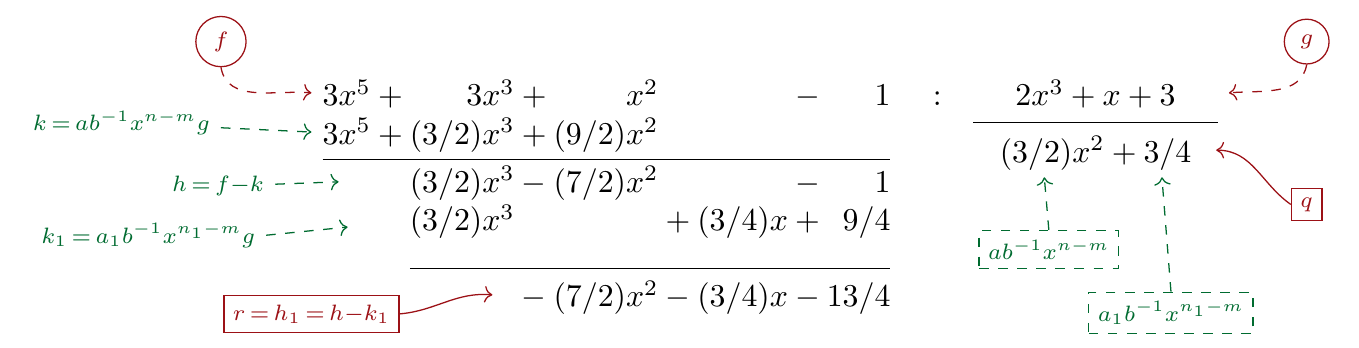
\includegraphics[scale=.4]{res/divisione_polinomiale}
	\end{center}
	
\end{example}

Un caso molto importante è quello dei polinomi a coefficienti in un campo. Infatti, se $A$ è un campo e $0_{A} \neq g \in A[x]$ allora $cd(g)$ è invertibile, come ogni elemento non nullo di $A$. Dunque, in questo caso, l'ipotesi $cd(g) \in \mathcal{U}(A)$ del teorema appena dimostrato può essere sostituita da $g \neq 0_{A}$. Il fatto che ogni polinomio a coefficienti in un campo non sullo sia divisibile ci permette di eseguire l'algoritmo euclideo delle divisioni successive.



\begin{example}
	Per quanto appena detto, se $F$ è un campo, è sempre possibile dividere un polinomio $f \in F[x]$ per un polinomio $g \in F[x] \setminus \{0_{F}\}$. Ad esempio, se $F=\mathbb{Z}_{7}[x]$, vediamo come si divide il polinomio $\overline{2}x^{2}+\overline{3}x+\overline{4}$ per il polinomio $\overline{3}x+\overline{4}$. Un primo modo è quello di effettuare la divisione come se fosse in $\mathbb{Q}[x]$:
	\medskip
	
	\begin{center}
		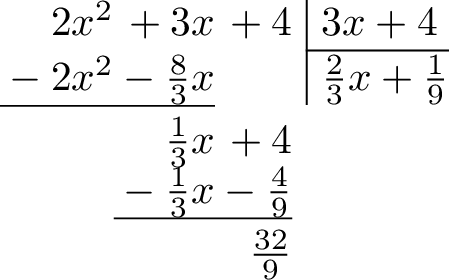
\includegraphics[scale=.25]{res/Divisionez7}
	\end{center}
	\medskip
	
	Quindi:
	\[\overline{2}x^{2}+\overline{3}x+\overline{4} =(\overline{3}x+\overline{4})\Biggl(\frac{\overline{2}}{\overline{3}}x+\frac{\overline{1}}{\overline{9}}\Biggr)+\frac{\overline{32}}{\overline{9}}\]
	Ma cosa sono $\frac{\overline{2}}{\overline{3}}$, $\frac{\overline{1}}{\overline{9}}$ e $\frac{\overline{32}}{\overline{9}}$? In $\mathbb{Z}_{7}$ si ha che $\overline{3}\cdot \overline{5}=\overline{15}=\overline{1}$, quindi $\overline{3}^{-1}=\overline{5}$. Dunque $\frac{\overline{2}}{\overline{3}}=\overline{10}=\overline{3}$. Similmente $\overline{9}^{-1}=\overline{4}$, quindi $\frac{\overline{1}}{\overline{9}}=\overline{4}$ e $\frac{\overline{32}}{\overline{9}}=\overline{32}\cdot \overline{4}=\overline{128}=\overline{1}$. Dunque:
	\[\overline{2}x^{2}+\overline{3}x+\overline{4} =(\overline{3}x+\overline{4})(\overline{3}x+\overline{4})+\overline{2}\]
\end{example}


\subsection{Applicazioni polinomiali}
Sia $f\in A[x]$, dove $A$ è un anello polinomiale. Se $f= \sum_{i=0}^{n} a_{i}x^{i}$ e $c \in A$ si ha:
\begin{displaymath}
	f(c) = \sum_{i=0}^{n} a_{i}c^{i}
\end{displaymath}

\begin{defbox}{Applicazione polinomiale}
	L'applicazione:
	\begin{equation}
		\widetilde{f} : c \in A \mapsto f(c) \in A
	\end{equation}
	che prende il nome di \textbf{applicazione polinomiale} determinata da $f$ in $A$.
\end{defbox}

\begin{osservation}
	A differenza dell'omomorfismo di sostituzione questa applicazione non è, in generale, un omomorfismo. osserviamo che se $f \in A$ allora $f(c)=f$ per ogni $c \in A$, quindi l'applicazione $\widetilde{f}$ è costante. È per questo motivo che gli elementi di $A$ vengono chiamati polinomi costanti.
\end{osservation}


\begin{defbox}{Radice}
	L'elemento $c \in A$ è una \textbf{radice} di $f$ se e solo se $f(c) = 0_{A}$.
\end{defbox}



\begin{lemmabox}\label{lemma:divisori_prodotto_polinomi}
	Siano $A$ un anello commutativo unitario e $f,g \in A[x]$. Allora:
	\begin{enumerate}
		\item se, in $A[x]$, $f$ divide $g$, ogni radice di $f$ in $A$ è radice di $g$.
		\item se $A$ è un dominio di integrità, allora le radici di $fg$ in $A$ sono tutti e soli gli elementi di $A$ che sono radici di $f$ o di $g$.
	\end{enumerate}
	
\end{lemmabox}

\begin{proof}
	\begin{enumerate}
		\item Se $f \divides_{A[x]} g$ esiste $h \in A[x]$ tale che $g=fh$. Allora applicando l'omomorfismo di sostituzione definito da $g$, abbiamo:
		\begin{displaymath}
			g(c) = f(c)h(c) = 0_{A}h(c)=0_{A}
		\end{displaymath}
		dunque $c$ è radice di $g$.
		\item Per la $(1)$, gli elementi di $A$ che sono radici di $f$ o $g$ sono radici anche di $fg$, multiplo di entrambi. Viceversa, se $c$ è radice di $A$ di $fg$, allora:
		\begin{displaymath}
			0_{A} = (fg)(c)=f(c)g(c)
		\end{displaymath}
		Poiché $A[x]$ è un dominio di integrità, questo implica che uno tra $f(c)$ e $g(c)$ è $0_{A}$, quindi $c$ è radice di uno tra $f$ e $g$.
	\end{enumerate}
\end{proof}

\begin{teorbox}[del resto]
	Sia $A$ un anello commutativo unitario e siano $f \in A[x]$ e $c \in A$. Allora $f(c)$ è il resto della divisione di $f$ per $x-c$.
\end{teorbox}

\begin{proof}
	La prima cosa da osservare è che si può certamente effettuare la divisione di $f$ per $x-c$, perché quest'ultimo polinomio è monico, quindi il suo coefficiente direttore è invertibile. Effettuata questa divisione, otteniamo $q,r \in A[x]$ tali che $f=(x-c)q+r$ e si ha $deg r < deg (x-c) =1$. Quest'ultima condizione equivale a dire che $r$ è un polinomio costante. Applichiamo l'omomorfismo di sostituzione:
	\begin{displaymath}
		f(c) = \bigl((x-c)q+r\bigr)(c)= (c-c)q(c)+r(c)=0_{A}q(c)+r=r
	\end{displaymath}
	
	È così provato che $f(c)=r$. 
\end{proof}

\begin{teorbox}[di Ruffini]\label{thm:ruffini}
	Sia $A$ un anello commutativo unitario e siano $f \in A[x]$ e $c \in A$. Allora $c$ è radice di $f$ se e solo se $(x-c)$ divide $f$ in $A[x]$, ovvero se e solo se il resto della divisione di $f$ per $(x-c)$ è zero.
\end{teorbox}

\begin{proof}
	Per il teorema del resto, $c$ è radice di $f$ se e solo se il resto della divisione di $f$ per $x-c$ è zero, cioè se e solo se $x-c$ divide $f$.
\end{proof}

\begin{example}
	Dato il polinomio $f(x)=x^{3}-2x^{2}-5x+10$ abbiamo che $f(2)=0$ e $f(\sqrt{5})$. Per il teorema di Ruffini, abbiamo che $x-2$ e $x-\sqrt{5}$ dividono $f(x)$. Abbiamo infatti:
	\[x^{3}-2x^{2}-5x+10=(x-2)(x^{2}-5=(x-2)(x-\sqrt{5})(x+\sqrt{5})\]
\end{example}


\begin{corolbox}
	Sia $A$ un anello commutativo unitario e siano $f,g \in A[x]$ e $c \in A$. Supponiamo che $f$ e $g$ abbiano in $A[x]$ un massimo comun divisore $d$. Allora le radici comuni a $f$ e $g$ in $A$ sono tutte e sole le radici di $d$ in $A$:
	\begin{equation}
		\{c \in A \; | \; f(c)=0_{A}=g(c)\}=\{c \in A \; | \; d(c)=0_{A}\}
	\end{equation}
\end{corolbox}

\begin{teorbox}[di Ruffini generalizzato]
	Sia $A$ un dominio di integrità unitario e siano $f \in A[x]$, $n \in \mathbb{N}^{*}$ e $c_{1},c_{2}, \ldots, c_{n} \in A$ degli elementi a due a due distinti. Allora si ha che ciascuno degli elementi $c_{i}$ è radice di $f$ se e solo se:
	\begin{displaymath}
		\prod_{i=1}^{n}(x-c_{i}) \divides_{A[x]} f
	\end{displaymath}
\end{teorbox}

\begin{proof}
\begin{itemize}
	\item[$\impliedby$] Ovvio. Se $\prod_{i=1}^{n}(x-c_{i})$ divide $f$ allora ciascuno degli elementi $c_{i}$ è radice di $f$, in quanto $x-c_{i}$ divide $f$.
	
	\item[$\implies$] Si procede per induzione su $n$. Supponiamo che gli elementi $c_{i}$ per ogni $i \in \{1,2,\ldots,n\}$ siano radici di $f$. Se $n=1$ allora $x-c_{1}$ divide $f$ per il teorema di Ruffini. Supponiamo allora $n>1$ e, come ipotesi di induzione, che l'enunciato valga per insiemi di $n-1$ elementi distinti di $A$ ed arbitrari polinomi in $A[x]$.
	
	Poiché $f(c_{n}) = 0_{A}$, per il teorema di Ruffini esiste $q \in A[x]$ tale che $f=(x-c_{n})q$. Sia ora $i$ un intero tale che $1 \leq i < n$. Poiché $c_{i}$ è radice di $f$ e $A$ è un dominio di integrità, segue che $c_{i}$ è radice di uno tra $x-c_{n}$ e $q$ (vedi Lemma \ref{lemma:divisori_prodotto_polinomi}). Dunque ciascuno degli elementi $c_{1},c_{2},\ldots, c_{n-1}$ è radice di $q$. Possiamo allora applicare l'ipotesi di induzione e concludere che: $$\prod_{i=1}^{n-1}(x-c_{i}) \divides_{A[x]} q$$ quindi esiste $h \in A[x]$ tale che:
	\begin{displaymath}
		q = h \prod_{i=1}^{n-1}(x-c_{i})
	\end{displaymath}
	Allora:
	\begin{align*}
		f &= q \cdot (x-c_{n}) \\
		  &= \Bigl( h \cdot \prod_{i=1}^{n-1}(x-c_{i})\Bigr) \cdot (x-c_{n}) \\
		  &= h \prod_{i=1}^{n}(x-c_{i})
	\end{align*}
	Pertanto $\prod_{i=1}^{n}(x-c_{i})$ divide $f$ in $A[x]$ e la dimostrazione è così completa.
\end{itemize}
\end{proof}

Il teorema di Ruffini generalizzato ha due importantissime conseguenze. La prima è una \textbf{limitazione al numero di radici che un polinomio non nullo su un dominio di integrità può avere}.

\begin{teorbox}\label{thm:grado_polinomio}
	Sia $A$ un dominio di integrità unitario e sia $0_{A} \neq f \in A[x]$. Allora il numero delle radici di $f$ in $A$ non supera $deg(f)$.
\end{teorbox}
\begin{proof}
	Se $f$ ha esattamente $n$ radici, siano esse $c_{1},c_{2},\ldots,c_{n}$ allora $f$ è multiplo di $g$:
	\begin{displaymath}
		g \coloneqq \prod_{i=1}^{n}(x-c_{i})
	\end{displaymath}
	Quindi $f = gq$ per un opportuno $q \in A[x]$. Essendo $f\neq 0_{A}$ si ha anche $q \neq 0_{A}$. Ma $deg(g) =n$ e per $g$ e $q$ vale la regola di addizione dei gradi. Quindi $deg(f) = deg(g) + deg (q) = n + deg (q) \geq n$, ovvero $n \leq deg(f)$.
\end{proof}


\begin{osservation}
	Sia per il teorema di Ruffini generalizzato che per il Teorema \ref{thm:grado_polinomio} è \textbf{essenziale l’ipotesi che l'anello sia un dominio di integrità}. Sia $f=\overline{2}x \in \mathbb{Z}_{6}[x]$. Sia $\overline{0}$ che $\overline{3}$ sono radici del polinomio, quindi $f$ ha più radici di quanto sia il suo grado, che è 1. Inoltre, come imposto dal teorema di Ruffini sia $x = x - \overline{0}$ che $x- \overline{3}$ dividono $f$. Infatti:
	\begin{align*}
		f = x \cdot \overline{2} = (x- \overline{3}) \cdot \overline{2}
	\end{align*}
Ma osserviamo che $x(x-\overline{3})$ non divide $f$, quindi la conclusione di Ruffini generalizzato \emph{non vale} per $f$.
\end{osservation}

L’altra conseguenza del teorema di Ruffini generalizzato riguarda le applicazioni polinomiali e ci dice che, \textbf{nel caso dei domini di integrità infiniti, ogni polinomio è identificato univocamente dalla sua applicazione polinomiale}.

\begin{propbox}
	Principio di identità dei polinomi
	Sia $A$ un dominio di integrità infinito. Allora, per ogni $f,g \in A[x]$ si ha:
	\begin{displaymath}
		\widetilde{f} = \widetilde{g} \iff f=g
	\end{displaymath}
\end{propbox}

\begin{proof}
	Ovviamente $\widetilde{f} = \widetilde{g}$ se $f=g$. Supponiamo, viceversa, $\widetilde{f} = \widetilde{g}$. Allora $f(c)=g(c)$ per ogni $c \in A$. Sia $h = f-g$. Allora, per ogni $c \in A$ abbiamo $h(c) = (f-g)(c)=f(c)-g(c)=0_{A}$, vale a dire: ogni elemento di $A$ è radice di $h$. Dunque $h$ ha un numero infinito di radici. Ma il Corollario precedente assicura che, se $h \neq 0_{A}$, allora il numero delle radici di $h$ non supera $deg(h)$, quindi è finito. Di conseguenza deve essere $h=0_{A}$, ovvero $f=g$.
\end{proof}


È a causa del principio di identità dei polinomi che in alcuni casi vengono identificati i polinomi con le applicazioni polinomiali. Ad esempio, nei corsi di analisi matematica si definiscono i polinomi come particolari funzioni da $\mathbb{R}$ a $\mathbb{R}$, quelle che per noi sono le applicazioni polinomiali definite dai polinomi in $\mathbb{R}[x]$. Questo è lecito perché, essendo $\mathbb{R}$ un campo (quindi un dominio di integrità) infinito, il principio di identità dei polinomi assicura che i polinomi in $\mathbb{R}[x]$ corrispondono esattamente alle loro applicazioni polinomiali (in corsi di analisi più avanzati i polinomi sono definiti con riferimento al campo complesso, anziché a quello reale; il discorso è analogo: anche per il campo complesso vale il principio di identità dei polinomi). D’altra parte, \emph{non è lecito identificare polinomi ed applicazioni polinomiali in contesti in cui non valga il principio di identità dei polinomi}, cioè quando l’anello $A$ considerato sia finito oppure non sia integro.


Nel caso degli anelli finiti è certo che il principio di identità dei polinomi non può valere. Infatti, se $A$ è un anello commutativo unitario finito, il numero delle applicazioni da $A$ ad $A$, e quindi il numero delle applicazioni polinomiali in $A$, è finito, mentre $A[x]$ è comunque infinito. Dunque, in questo caso, è impossibile che ci sia una corrispondenza biunivoca tra polinomi e applicazioni polinomiali (ciò che il principio di identità dei polinomi afferma è che, se $A$ è un dominio di integrità infinito, l’applicazione $f \in A[x] \mapsto  \widetilde{f} \in Map(A, A)$ è iniettiva; ciò è impossibile nel caso che stiamo considerando ora, in cui il dominio $A[x]$ è infinito ma il codominio $Map(A, A)$ è finito).


\begin{example}
	Consideriamo il polinomio $f= x^{3}-x \in \mathbb{Z}_{3}[x]$. Si ha:
	\begin{align*}
		\overline{f}([0]_{3}) &= \overline{0}^{3}-\overline{0} = \overline{0}\\
		\overline{f}([1]_{3}) &= \overline{1}^{3} - \overline{1} = \overline{0}\\
		\overline{f}([2]_{3}) &= \overline{2}^{3} -\overline{2} = \overline{8}-\overline{2}=\overline{6}=\overline{0}
	\end{align*}
	Quindi $\overline{f} = \overline{0}$ ma $f \neq \overline{0}$.
\end{example}

\subsection{Fattorizzazione}

Ricordiamo che un monoide commutativo cancellativo (cioè ad elementi tutti cancellabili) si dice \textbf{fattoriale} se e
solo se ogni suo elemento non invertibile è prodotto di elementi irriducibili e tali decomposizioni in irriducibili
sono essenzialmente uniche.


\begin{teorbox}
	Se $A$ è un anello fattoriale allora $A[x]$ è fattoriale.
\end{teorbox}


Sono certamente fattoriali i campi ed è fattoriale, per il Teorema Fondamentale dell’Aritmetica, l’anello $\mathbb{Z}$ degli interi. Quindi è fattoriale $\mathbb{Z}[x]$ e, per ogni campo $K$, anche $K[x]$. Dunque, sia per i polinomi a coefficienti in $\mathbb{Z}$ che per quelli a coefficienti in un campo vale un teorema di fattorizzazione essenzialmente unica in prodotto di polinomi irriducibili: \textit{ogni polinomio non invertibile e non nullo è prodotto di polinomi irriducibili e tale fattorizzazione è unica a meno dell’ordine dei fattori e della sostituzione di alcuni fattori con polinomi associati.}



Se $K$ è un campo, si ha:
\begin{displaymath}
	\mathcal{U}(K[x]) = \mathcal{U}(K) = K \setminus \{0_{K}\}
\end{displaymath}
Quindi l'insieme di tutti i polinomi associati ad un $f \in K[x] \setminus \{0_{K}\}$ è:
\begin{displaymath}
	\{uf \; | \; u \in K \setminus \{0_{K}\} \}
\end{displaymath}
Se $a = cd(f)$, si ha $cd(uf)=ua$ per ogni $u \in K \setminus \{0_{K}\}$. Allora, qualunque sia $k \in K \setminus \{0_{K}\}$, il polinomio $f$ ha esattamente un associato con coefficiente direttore $k$, precisamente $(ka^{-1})f$. Infatti, per ogni $u \in K \setminus \{0_{K}\}$ abbiamo che $cd(uf) =ua = k$ se, e solo se, $c = ka^{-1}$.

\begin{propbox}
	Sia $K$ un campo. In ogni classe di elementi associati di polinomi non nulli in $K[x]$ esiste uno ed un solo polinomio monico che prende il nome di \textbf{rappresentante monico}.
\end{propbox}


\begin{example}
	In $\mathbb{Q}[x]$ il polinomio monico associato a $f = 3x^{2}+x-6$ è:
	\begin{displaymath}
		(\frac{1}{3})f = x^{2}+ \frac{1}{3}x -2
	\end{displaymath}
	ma anche:
	\begin{displaymath}
		-6x^{2}-2x+12
	\end{displaymath}
	e infiniti altri polinomi della forma $uf$, dove $0 \neq u \in \mathbb{Q}$.
\end{example}

\begin{propbox}
	Sia $K$ un campo. Allora ogni polinomio non nullo in $K[x]$ è prodotto di un elemento di $K$ e di polinomi monici irriducibili in $K[x]$. Tale fattorizzazione è unica a meno dell’ordine dei fattori.
\end{propbox}

\begin{proof}
	L'unicità della fattorizzazione segue dal fatto che $K[x]$ è fattoriale e dal fatto che ogni classe di polinomi associati non nullo contiene un solo rappresentante monico. L'esistenza della decomposizione è ovvia nel caso dei polinomi costanti, va provata per polinomi non costanti. Sia, allora $f \in K[x] \setminus K$. Sia $f=p_{1}p_{2}\cdot \ldots \cdot p_{n}$ una fattorizzazione di $f$ in prodotto di polinomi irriducibili. Per ogni $i \in \{1,2,\ldots, n\}$ sia $a_{i} = cd (p_{i})$; allora $p_{i}=a_{i}q_{i}$, dove $q_{i}=a_{i}^{-1}p_{i}$ è associato a $p_{i}$ (quindi è irriducibile) ed è monico. Posto $a= a_{1}a_{2}\cdot \ldots \cdot a_{n}$ abbiamo $f=aq_{1}q_{2}\ldots q_{n}$. Questa è la decomposizione cercata.
\end{proof}

\begin{osservation}
	Nell’ipotesi che $A$ sia fattoriale, una delle conseguenze del fatto che $A[x]$ è fattoriale è che, nota una fattorizzazione in prodotto di irriducibili di un polinomio $f$, è facile determinare l’insieme dei divisori di $f$. Posto infatti $f=p_{1}^{\lambda_{1}} \cdot p_{2}^{\lambda_{2}} \cdot \ldots \cdot p_{n}^{\lambda_{n}}$, dove i $p_{i}$ sono polinomi irriducibili e per ogni $i \neq j$ $p_{i}$ e $p_{j}$ non sono associati, l'\textbf{insieme dei divisori} di $f$ è dato da tutti i polinomi della forma:
	\[
	p_{1}^{\sigma_{1}} \cdot p_{2}^{\sigma_{2}} \cdot \ldots \cdot p_{n}^{\sigma_{n}}
	\]
	ed i loro associati, dove, per ogni $i$, $\sigma_{i} \in \mathbb{N}$ e $\sigma_{i} \leq \lambda_{i}$.
\end{osservation}

Quindi, ogni polinomio non nullo di grado diverso da zero a coefficienti su un campo $K$ (ciò vale a dire: ogni elemento non zero e non invertibile di $K[x]$) si fattorizza in modo essenzialmente unico come prodotto di polinomi irriducibili. Poiché ogni classe di polinomi irriducibili associati contiene uno ed un solo polinomio monico, possiamo concludere che, se $K$ è un campo, allora ogni polinomio $f \in K[x]\setminus K$ si scrive in modo unico (a meno dell'ordine dei fattori) come:
\[
f= a_{n} f_{1} f_{2} \ldots f_{k}
\]
dove $a_{n}$ è il coefficiente direttore di $f$ e $f_{1},f_{2}, \ldots, f_{k}$ sono polinomi monici irriducibili in $K[x]$. Ci vogliamo ora occupare di descrivere, per quanto possibile, la proprietà di essere o meno \textbf{irriducibile} per un polinomio a coefficienti in un campo. Vedremo in che modo questo proprietà è collegata alla presenza di radici.


\begin{example}
	In $\mathbb{Q}[x]$, $x^{2}-1$ ammette la fattorizzazione:
	\begin{displaymath}
		x^{2}-1 = (x-1)(x+1)
	\end{displaymath}
	In realtà $x^{2}-1$ ammette altre decomposizioni, come $(\frac{1}{2}x-\frac{1}{2})\cdot(2x+2)$. Tuttavia $x+1$ e $2x+2$ sono associati, differiscono cioè per un fattore invertibile. Allo stesso modo $x-1$ e $\frac{1}{2}x-\frac{1}{2}$ sono associati. Quindi sostanzialmente le due decomposizioni sono la stessa.
\end{example}

\begin{propbox}[Criterio di irriducibilità]
	Siano $K$ un campo e $f \in K[x]$. Se $n= deg(f)$ allora $f$ è irriducibile in $K[x]$ se e solo se $n>0$ e vale una delle due proprietà equivalenti:
	\begin{enumerate}
		\item non esistono $g,h \in K[x]$ tali che $f=gh$ e sia $g$ che $h$ abbiano grado minore di $n$;
		\item non esistono $g,h \in K[x]$ tali che $f=gh$ e sia $g$ che $h$ abbiano grado maggiore di $0$.
	\end{enumerate}
\end{propbox}

\begin{proof}
Ricordiamo che $f$ è irriducibile se e solo se, in $K[x]$, non è invertibile e non ha divisori se non
	quelli banali. Possiamo subito osservare che i polinomi costanti non sono irriducibili. Infatti i polinomi costanti non nulli sono invertibili, mentre il polinomio nullo ha tutti gli elementi di $K[x] \setminus K$ come divisori non banali. Abbiamo così che l’asserto è corretto nel caso in cui $f$ sia costante: $f$ non è irriducibile e non è vero che $n = deg(f) > 0$, quindi la condizione all’enunciato non è soddisfatta. 
	
	Possiamo allora assumere $f \notin K$, cioè: $n > 0$. Supponiamo dunque $n > 0$. osserviamo che, se $g,h \in K[x]$ e $f=gh$, per la regola di addizione dei gradi (che vale perché $K$ è un campo) si ha:
	$$n=deg(f)=deg(g)+deg(h)$$
	Quindi $deg(g)<n$ e $deg(h)<n$ che è equivalente alla condizione $(deg(g)>0 \land deg(h)>0)$, vale a dire che la (1) e la (2) sono equivalenti. 
	
	Se $f$  è irriducibile, scelti comunque $g,h \in K[x]$ tali che $f=gh$, allora $g$ è un divisore di $f$, quindi un divisore banale perché $f$ è irriducibile. Allora o $g$ è invertibile, nel qual caso $g \in K \setminus \{0_{K}\}$ e $deg(g)=0$, oppure $g$ è associato ad $f$, nel qual caso $deg(g)=deg(f)=n$. Ciò mostra che, se $f$ è irriducibile, sono verificate (1) e (2). 
	
	Se invece $f$ non è irriducibile, $f$ ha un divisore non banale $g$, allora $g \neq 0_{K}$ e $g$ non è invertibile, quindi $deg(g)>0$ ed esiste $h \in K[x]$ tale che $f=gh$. Ovviamente $h \neq 0_{K}$ e $h$ non è invertibile perché $g$ non è associato ad $f$, quindi abbiamo anche $deg(h)>0$. In questo caso, dunque, non vale (2) e quindi neanche (1).
\end{proof}


\begin{osservation}
	Un’ovvia conseguenza di questa caratterizzazione è che \textit{i polinomi di primo grado a coefficienti in un campo $K$ sono certamente irriducibili in $K[x]$}, dal momento che i prodotti tra polinomi di grado minore di $1$ sono certamente costanti.
\end{osservation}



\begin{propbox}
	Sia $K$ un campo e sia $f \in K[x]$. Allora $f$ ha radici in $K$ se e solo se ha almeno un divisore di primo grado in $K[x]$.
\end{propbox}


\begin{propbox}
	Sia $A$ un dominio di integrità unitario e sia $f \in A[x]$. Se $deg(f) > 1$ e $f$ ha radici in $A$, allora $f$ è riducibile in $A[x]$.
\end{propbox}

\begin{propbox}
	Siano $K$ un campo e $f$ un polinomio in $K[x]$ di grado 2 o 3. Allora $f$ è irriducibile in $K[x]$ se e solo se è privo di radici in $K$.
\end{propbox}

Possiamo schematizzare come segue le informazioni ottenute sulle proprietà di un polinomio a coefficienti in un campo di essere o meno irriducibile ed di avere o meno radici. Se $K$ è un campo e $0_{K} \neq f \in K[x]$, posto $deg(f) = n$ si ha:
\begin{center}
	\begin{tblr}{hlines,cells={mode=math},colspec={|ccl|}}
		n = 0 & \implies & \text{$f$ è invertibile e privo di radici} \\
		n = 1 & \implies & \text{$f$ è irriducibile ed ha una radice}\\
		n \in \{2,3\} & \implies & \text{$f$ irriducibile} \iff \text{$f$ non ha radici} \\
		n>3 & \implies &  \text{$f$ irriducibile} \implies \text{$f$ non ha radici}
	\end{tblr}
	\captionof{table}{Irriducibilità di un polinomio in un campo}\label{tab:irridicibili}
\end{center}

\subsection{Metodi ed esempi di fattorizzazione per polinomi su un campo}
Supponiamo di voler fattorizzare un polinomio (in un fissato anello di polinomi) in prodotto di polinomi irriducibili. Per farlo abbiamo bisogno:
\begin{itemize}
	\item di saper trovare divisori non banali del polinomio dato, se ne esistono;
	\item di saper riconoscere quali tra questi divisori sono irriducibili.
\end{itemize}

Limitiamoci al caso dei polinomi su un campo. Usando la tabella nella sezione precedente, sappiamo, in linea di
massima, rispondere al secondo punto nel caso di divisori di grado minore di quattro. I polinomi di grado uno
sono sempre irriducibili, quelli di grado due o tre lo sono se e solo se sono privi di radici. In due casi notevoli
queste informazioni sono addirittura più di quanto non sia necessario. Infatti valgono questi teoremi (che non
dimostriamo) per polinomi in $\mathbb{R}[x]$.

\begin{teorbox}
	Ogni polinomio irriducibile in $\mathbb{R}[x]$ ha grado minore di 3.
\end{teorbox}


Dunque, i polinomi irriducibili in $\mathbb{R}[x]$ sono precisamente quelli di grado 1 e quelli di grado 2 privi di radici. Come è noto dalle scuole superiori, un polinomio $ax^{2} + bx + c \in \mathbb{R}[x]$ di grado 2 ha radici in $\mathbb{R}$ se e solo se $b^{2}- 4ac \geq 0 $.

\begin{teorbox}[di Bolzano]
	Ogni polinomio di grado dispari in $\mathbb{R}[x]$ ha qualche radice in $\mathbb{R}$.
\end{teorbox}

La situazione è molto più complessa (ed interessante) nel caso di polinomi in $\mathbb{Q}[x]$. Lo studio dei polinomi in $\mathbb{Q}[x]$ si può ridurre al caso dei polinomi a coefficienti interi. Ricordiamo che $\mathbb{Z}[x]$ è un dominio di integrità, così come $\mathbb{Q}[x]$, ma gli unici elementi invertibili di $\mathbb{Z}[x]$ sono $\pm 1$, cioè gli stessi di $\mathbb{Z}$. Inoltre i polinomi di $\mathbb{Z}[x]$ che dividono un intero $a_{0} \neq 0$ devono avere grado zero, cioè solo a loro volta interi. Dunque:
\begin{itemize}
	\item $a_{0}$ ha gli stessi divisori in $\mathbb{Z}[x]$ e $\mathbb{Z}$;
	\item in particolare $a_{0}$ è invertibile in $\mathbb{Z}[x]$ se e solo se è invertibile in $\mathbb{Z}$, cioè se e solo se è $\pm 1$;
	\item per $a_{0} \neq \pm 1$, $a_{0}$ ha le stesse decomposizioni in prodotto di fattori irriducibili in $\mathbb{Z}[x]$ e in $\mathbb{Z}$.
\end{itemize}

\begin{defbox}{Polinomio primitivo}
	Sia $f(x)$ un polinomio a coefficienti interi. Si dice che $f(x)$ è primitivo se il massimo comun divisore dei suoi coefficienti è 1.	Un polinomio monico intero è primitivo.
\end{defbox}

\begin{teorbox}
	Ogni polinomio $f \in \mathbb{Q}[x]$ è associato, in $\mathbb{Q}[x]$ ad un polinomio $\overline{f} \in \mathbb{Z}[x]$.
\end{teorbox}

\begin{example}
	Ad ogni polinomio $b(x) \in \mathbb{Q}[x]$ è associato un polinomio primitivo $a(x) \in \mathbb{Z}[x]$ ottenuto moltiplicando $b(x)$ per il minimo comune multiplo dei suoi coefficienti e successivamente dividendo il polinomio così ottenuto per il massimo comun divisore dei coefficienti. Ad esempio, il polinomio $f(x) = \frac{1}{2}x^{2}+\frac{3}{4}x+\frac{1}{3}$ è associato al polinomio primitivo $g(x) = \frac{12}{2}x^{2}+\frac{12 \cdot 3}{4}x+\frac{12}{3}=6x^{2}+9x+4$.
\end{example}

Ora, polinomi tra loro associati hanno esattamente le stesse proprietà rispetto alla fattorizzazione.

\begin{propbox}[Criterio di Eisenstein]
	Sia $f= a_{0}+a_{1}x+a_{2}x^{2}+ \ldots + a_{n}x^{n} \in \mathbb{Z}[x]$. Se esiste un primo $p \in \mathbb{P}$ tale che:
	\begin{enumerate}
		\item $p$ divide $a_{0},a_{1}, \ldots, a_{n-1}$
		\item $p$ non divide $a_{n}$
		\item $p^{2}$ non divide $a_{0}$
	\end{enumerate}
	allora $f$ è irriducibile in $\mathbb{Q}[x]$.
\end{propbox}

\begin{osservation}
	Per ogni intero positivo $n$ e per ogni primo $p$, il polinomio $x^{n} - p$ è irriducibile in $\mathbb{Q}[x]$ e dunque in $\mathbb{Q}[x]$ ci sono polinomi irriducibili di ogni grado.
\end{osservation}


\begin{teorbox}[delle radici razionali]\label{prop:car_radici_Q}
	Sia $f=a_{n}x^{n}+a_{n-1}x^{n-1}+\ldots+a_{2}x^{2}+ a_{1}x +a_{0} \in \mathbb{Z}[x]$, un polinomio a coefficienti interi con $a_{n} \neq 0$. Allora ogni soluzione razionale di $f$ (ogni radice in $\mathbb{Q}$) si scrive come frazione $u/v$, dove $u$ e $v$ sono interi coprimi e $u$ è un divisore del termine noto $a_{0}$ e $v$ è un divisore del coefficiente direttore $a_{n}$.
\end{teorbox}

\begin{proof}
	Ogni numero razionale si può scrivere come frazione ridotta, quindi nella forma $u/v$, dove $u$ e $v$ sono interi coprimi e $v \neq 0$. Se una tale frazione $u/v$ è radice di $f$ allora:
	\begin{displaymath}
		0 = a_{0}v^{n} + a_{1}uv^{n-1} + a_{2}u^{2}v^{n-2}+ \ldots + a_{n-2}u^{n-2}v^{2}+ a_{n-1}u^{n-1}v + a_{n}u^{n}=0
	\end{displaymath}
	Ora, escluso (per il momento) il primo, tutti gli addendi a primo membro sono multipli di $u$. Poiché la loro somma vale 0, il primo addendo $a_{0}v^{n}$ è l'opposto della somma dei rimanenti. Quindi anch'esso è un multiplo di $u$. Dunque $u$ divide $a_{0}v^{n}$. Ma $u$ è coprimo con $v$, quindi con $v^{n}$, dunque $u$ divide $a_{0}$. In modo analogo $v$ divide $a_{n}$.
\end{proof} 

\begin{osservation}
	Ogni polinomio in $\mathbb{Q}[x]$ è associato (in $\mathbb{Q}[x]$) ad un polinomio in $\mathbb{Z}[x]$, che avrà le stesse radici razionali. 
\end{osservation}

Quindi, per cercare le radici razionali di un polinomio in $\mathbb{Q}[x]$ possiamo cercare le radici razionali del suo associato in $\mathbb{Z}[x]$. Questo è un vantaggio perché, come abbiamo visto, la ricerca delle radici razionali di un polinomio in $\mathbb{Z}[x]$ è semplificata dal criterio di Eisenstein e dalla proposizione \ref{prop:car_radici_Q}.
 
Volendo ricercare le radici razionali di un polinomio $f \in \mathbb{Q}[x]$ possiamo quindi procedere come segue:
\begin{enumerate}
	\item Sostituiamo il polinomio con un suo associato a coefficienti interi;
	\item Si considera il coefficiente direttore $a_{n}$ ed il termine noto $a_{0}$ del polinomio.
	\item Le radici razionali del polinomio sono le frazioni della forma $u/v$ con $u$ e $v$ interi coprimi tali che $u$ divida $a_{0}$ e $v$ divida $a_{n}$.
\end{enumerate}

È chiaro che (escluso il caso, banalmente semplificabile, in cui $a_{0}=0$) esiste solo un numero finito di tali frazioni, possiamo allora verificare per ciascuna di esse se è o meno radice del polinomio.


\begin{example}
	Consideriamo il polinomio $f=x^{4}-4x^{2}+(3/2)x+3 \in \mathbb{Q}[x]$. Un suo associato a coefficienti interi è: $$2f=2x^{4}-8x^{2}+3x+6$$
	con coefficiente direttore $2$ e termine noto $6$. Le frazioni della forma $\frac{u}{v}$ con $u$ e $v$ interi coprimi tali che $u$ divida $6$ e $v$ divida $2$ sono: $1=\frac{1}{1}$, $\frac{1}{2}$, $2$, $3$, $\frac{3}{2}$, $6$ e i loro opposti. 
	
	Per cercare tutte le radici razionali di $f$ non dobbiamo fare altro che \textit{controllare quali di questi dodici numeri sono radici di $f$ in $\mathbb{Q}[x]$}. Nel nostro caso la verifica diretta mostra che solo $-2$ è radice. Concludiamo che $-2$ è l'unica radice in $\mathbb{Q}[x]$.
	
	Possiamo proseguire lo studio di questo polinomio cercando di fattorizzarlo in prodotto di irriducibili. Usiamo il Teorema di Ruffini; dividendo $f$ per $x+2$ (cioè $(x-(-2))$) otteniamo: $$f=(x+2)(x^{3}-2x^{2}+3/2)$$
	
	Il secondo fattore $f_{1}$ di questo prodotto è associato a $2f_{1}=2x^{3}-4x^{2}+3$. Sfruttando la proposizione \ref{prop:car_radici_Q} concluderemmo che le radici di $f_{1}$ sono da cercare tra le frazioni ridotte della forma $u/v$ dove $u,v \in \mathbb{Z}$, $u$ divide 3 e $v$ divide 2. 
	
	In realtà non è necessario esaminare tutte queste frazioni perché ogni radice di $f_{1}$ è anche radice di $f$ e di tutte queste frazioni, tranne -2, sappiamo che non sono radici di $f$, quindi nemmeno di $f_{1}$. Dobbiamo esaminare solo $-2$, si ha: $$f_{1}(-2)=(-2)^{3}-2(-2)^{2}+3/2\neq 0$$quindi $-2$ non è radice di $f_{1}$. Pertanto $f_{1}$ non ha radici in $\mathbb{Q}$; poiché $deg(f)=3$ concludiamo che $f_{1}$ è irriducibile in $\mathbb{Q}[x]$. 	Dunque una fattorizzazione (l'unica a meno dell'ordine) di $f$ in prodotto di irriducibili monici in $\mathbb{Q}[x]$ è: \[f=(x+2)(x^{3}-2x^{2}+3/2)\]
\end{example}
\marker{yellow!50}{yellow!20!black}{Quando la cardinalità del campo	finito $F$ è piccola il metodo più efficace per la ricerca delle radici di un polinomio $f \in F[x]$ è spesso la verifica diretta eseguita per ogni elemento, vale a dire il calcolo di $f(c)$ per ogni elemento $c$ del campo.}
\newpage
\section{Esercizi svolti}
\subsection{Aritmetica e congruenze}
\begin{exsbox}
	Determinare il più grande numero naturale $k<100$ per cui ammette soluzione l'equazione diofantea $8x+12y=k$ e risolverla.
\end{exsbox}

\paragraph{Svolgimento.} Sappiamo che una equazione diofantea è risolubile se il massimo comune divisore tra i due coefficienti delle incognite divide il termine noto.

In questo caso $MCD(8,12)=4$ e il più grande numero naturale, minore di 100 e multiplo di 4 è 96. L'equazione diofantea diventa quindi:
\[8x+12y=96\]
Per il Teorema di Bezout possiamo esprimere 4 come combinazione lineare di 8 e 12 e abbiamo:
\[4 = 8 \cdot -1 + 12 \cdot 1\]
Quindi la coppia $(-1,1)$ è soluzione dell'equazione diofantea $8x+12y=4$. Essendo $96= 4 \cdot 24$, moltiplicando la coppia $(-1,1)$ per 24 si ottiene la coppia $(-24,24)$ che è la soluzione ricercata. \hfill \blacksquare

\begin{exsbox}
	Determinare l'insieme $X=\{n \in \mathbb{Z} / 16(1-n) \equiv_{36} 12n+a\}$ per almeno un $a \in \{6,7,8,9\}$.
\end{exsbox}
\paragraph*{Svolgimento.} Per come è stato definito l'insieme $X$ possiamo dare una descrizione di tale insieme più estesa, ovvero:
\begin{align*}
	X = \{n \in \mathbb{Z} / 16(1-n) \equiv_{36} 12n+ 6 \} \cup \{n \in \mathbb{Z} / 16(1-n) \equiv_{36} 12n+ 7\} \\
	\cup \{n \in \mathbb{Z} / 16(1-n) \equiv_{36} 12n+8\} \\
	\cup \{n \in \mathbb{Z} / 16(1-n) \equiv_{36} 12n+9\}
\end{align*}
L'insieme $X$ è costituito quindi dagli interi che sono soluzione delle quattro equazioni congruenziali. L'equazione congruenziale generica è:
\begin{equation}\label{eq:esercizio_congruenze1}
	16(1-n) \equiv_{36} 12n+a
\end{equation}
con $a \in \{6,7,8,9\}$. Risolvere l'equazione \ref{eq:esercizio_congruenze1} significa ricercare i numeri interi tali che:
\begin{align*}
	36 \divides 16(1-n) - (12n+a) &\iff \exists k \in \mathbb{Z} \bigl(16(1-n) - (12n+a) = k \cdot 36 \bigr) \\
	&\iff \exists k \in \mathbb{Z} \bigl(16-16n - 12n -a = k \cdot 36 \bigr) \\
	&\iff \exists k \in \mathbb{Z} \bigl(16-28n -a = k \cdot 36 \bigr) & \text{\textcolor{gray}{Svolgendo l'espressione algebrica}}\\
	&\iff \exists k \in \mathbb{Z} \bigl((16-a) -28n = k \cdot 36\bigr) \\
\end{align*}
La ricerca delle soluzioni si riduce quindi alla risoluzione delle quattro equazioni congruenziali:
\begin{eqnarray}
	28n \equiv_{36} 16-6  \iff 28n \equiv_{36} 10 \\
	28n \equiv_{36} 16-7  \iff 28n \equiv_{36} 9\\
	28n \equiv_{36} 16-8  \iff 28n \equiv_{36} 8 \label{eq:esercizio_congruenze_risolubile}\\
	28n \equiv_{36} 16-9 \iff 28n \equiv_{36} 7
\end{eqnarray}
Procediamo quindi con la risoluzione della prima equazione. Il massimo comun divisore tra 28 e 36 è 4 e $4 \ndivides 10$, quindi la prima soluzione non ammette soluzioni per $a=6$. Analogamente per $a=7$ e $a=9$. Procediamo con l'equazione \ref{eq:esercizio_congruenze_risolubile} in quanto $(28,36) \divides 8$. Dividendo l'equazione per il massimo comune divisore si ottiene l'equazione congruenziale equivalente:
\begin{displaymath}
	7n \equiv_{9} 2
\end{displaymath}
Infatti sappiamo che le soluzioni di $28n \equiv_{36} 8$ sono tutte e sole quelle di $\frac{28}{4}n \equiv_{\frac{36}{4}} \frac{8}{4}$, ovvero $7n \equiv_{9} 2$, in quanto $4$ risulta essere un divisore comune di $28$, $36$ e $8$. Il vantaggio di tale semplificazione è dato dal fatto che $[7]_{9}$ è invertibile in $\mathbb{Z}_{9}$ in quanto $(7,9)=1$, ovvero 7 e 9 sono coprimi. Sfruttando il \hyperlink{thm:bezout}{Teorema di Bezout} possiamo quindi trovare un inverso di 7 in $\mathbb{Z}_{9}$. Esistono infatti due interi $u,v$ tali che: $1 = 7u+9v$. Chiaramente $1 = 28-27 =7 \cdot 4 - 9 \cdot 3$ e quindi $7 \cdot 4 -1 = 9 \cdot (-3)$. Abbiamo così dimostrato che la coppia $(4,-3)$ è una soluzione dell'equazione diofantea $1=7u+9v$. Moltiplicando per 2 si ottiene $2=7 \cdot 8  + 9 \cdot (-6) =56-54$ e si ha: $7 \cdot 8 -2 = 9 \cdot (-6)$, ovvero $9 \divides 7 \cdot 8 - 2$, cioè  $7 \cdot 8 \equiv_{9} 2$. Quindi $n=8$ è una soluzione dell'equazione $7n \equiv_{9} 2$, che è equivalente a dire che la classe di resto $[8]_{9}$ è una soluzione di tale equazione.

Concludiamo quindi dicendo che $X = \{n \in \mathbb{Z} / \exists k \in \mathbb{Z} (n = 9k+ 8)\}$. \hfill \blacksquare

\begin{exsbox}
	Verificare che l'insieme $\mathbb{Z}_{3}$ munito dell'operazione di addizione è un gruppo commutativo.
\end{exsbox}

\paragraph{Svolgimento.} Per dimostrare che $(\mathbb{Z}_{3},+)$ sia un gruppo commutativo dobbiamo dimostra che $(\mathbb{Z}_{3},+)$ risulta essere un monoide commutativo e che per ogni elemento di tale struttura esista l'opposto.
Come sappiamo $(\mathbb{Z}_{3},+)$ risulta essere una struttura algebrica definita dall'operazione indotta dalla relazione $\equiv_{3}$ nella struttura $(\mathbb{Z},+)$. Dai risultati\footnote{Vedi \ref{sez:congruenze}} dimostrati per le congruenze sappiamo che $+_{\equiv_{3}}$ conserva l'associatività e la commutatività. Quindi $(\mathbb{Z}_{3},+)$ è un semigruppo commutativo. Inoltre, preso $0 \in \mathbb{Z}$ elemento neutro in $(\mathbb{Z},+)$ si ha che $[0]_{3}$ risulta essere l'elemento neutro in $(\mathbb{Z}_{3},+)$ che risulta quindi un monoide commutativo. Se $-a \in \mathbb{Z}$ è l'opposto di $a \in \mathbb{Z}$ secondo l'operazione $+$ allora $[-a]_{3} = [a]_{3}$ è l'opposto dell'elemento $[a]_{3} \in \mathbb{Z}_{3}$ e $(\mathbb{Z}_{3},+)$ è quindi un gruppo abeliano. \hfill \blacksquare

\begin{exsbox}
	Si determinino le soluzioni della congruenza: $324x \equiv_{508} 127$.
\end{exsbox}
\paragraph*{Svolgimento.} L'equazione $324x \equiv_{508} 127$ non ha soluzioni. Infatti, calcolato  $MCD(324,508)=2$ si osserva che $2 \ndivides 127$. \hfill \blacksquare

\begin{exsbox}
	Si determinino le soluzioni della congruenza $3x \equiv_{8} 5$.
\end{exsbox}

\paragraph*{Svolgimento.}
Sappiamo che la congruenza ammette soluzioni intere poiché il massimo comun divisore tra 3 ed 8 è 1 che divide 5. Per determinare una soluzione scrivo 1 come combinazione linare di tre ed otto, risolvo cioè l'equazione diofantea:
\begin{displaymath}
	3x+8y=1
\end{displaymath}
Chiaramente, dalla divisione euclidea abbiamo:
\begin{displaymath}
	\left \lbrace
	\begin{array}{l}
		8 = 3 \cdot 2 + 2 \\
		3 = 2 \cdot 1 + 1 \\
	\end{array}
	\right .
	\implies
	\left\lbrace
	\begin{array}{l}
		2 = 8 - 3 \cdot 2\\
		1 = 3 - 2
	\end{array}
	\right .
\end{displaymath}
Quindi:
\begin{align*}
	1	&=  3 -  2  \\
	&= 3 -( 8-3 \cdot 2)\\
	&= 3 + 3 \cdot 2 - 8 \\
	&= 3 \cdot 3 -8 \\
	&= 3 \cdot 3 + (-1) \cdot 8
\end{align*}
Moltiplicando per 5 abbiamo che:
\begin{displaymath}
	5 = 15 \cdot 3 + (-5) \cdot 8
\end{displaymath}
e quindi $3 \cdot 15 \equiv_{8} 5$, ovvero ogni intero congruo a 15 (e cioè congruo a 7) modulo 8 è soluzione della congruenza. Dalla teoria sappiamo poi che l'insieme di tutte le soluzioni è costituito dagli interi congrui (modulo 8) a:
\begin{displaymath}
	x_{0} + t \cdot \frac{8}{(3,8)} =7+8t
\end{displaymath}
al variare di $0 \leq t < (3,8)=1$. Pertanto solo per $t=0$ si hanno soluzioni e queste sono dunque tutti e soli gli interi congrui a 7 modulo 8, ovvero la classe di resto $[7]_{8}$. \hfill \blacksquare
\begin{exsbox}
	Trovare le soluzioni dell'equazione congruenziale $87x \equiv_{12} 27$.
\end{exsbox}
\paragraph{Svolgimento.} Applicando l'algoritmo euclideo delle divisioni successive abbiamo che:
\begin{displaymath}
	\begin{array}{l}
		87 = 7 \cdot 12 + 3\\
		12 = 4 \cdot 3 + 0
	\end{array}
\end{displaymath}
Pertanto $MCD(87,12)=3$ e $3 \divides 27$. Quindi la congruenza ammette tre soluzioni. Risolviamo l'equazione diofantea $$87x+12y=27$$ Chiaramente $27 = 3 \cdot 9$, quindi:
\begin{align*}
	27 &= 9 \cdot 3 \\
	&= 9 \cdot (87 - 7 \cdot 12)\\
	&= 9 \cdot 87 - 63 \cdot 12\\
	&= 9 \cdot 87 + (-63) \cdot 12
\end{align*}
Dunque 9 è soluzione e tale è anche ogni intero congruo a 9 modulo 12. Le altre eventuali soluzioni, modulo 12 sono date da:
\begin{displaymath}
	9 + t \cdot \frac{12}{(87,12)} = 9+t \cdot 4
\end{displaymath}
con $0 \leq t < 3$ e pertanto le soluzioni modulo 12 della congruenza di partenza sono:
\begin{displaymath}
	\begin{cases}
		9 + 0 \cdot 4 = 9 \implies [9]_{12}\\
		9 + 1 \cdot 4 = 13 \implies [13]_{12} = [1]_{12}\\
		9 + 2 \cdot 4 = 17 \implies [17]_{12} = [5]_{12}
	\end{cases}
\end{displaymath}
\begin{flushright}
	\blacksquare
\end{flushright}

\begin{exsbox}
	Trovare le soluzioni dell'equazione congruenziale $87x+32 \equiv_{100} x+4$.
\end{exsbox}
\paragraph{Svolgimento.} Affermare che $87x+32 \equiv_{100} x+4$ è equivalente a dire:
\begin{align*}
	100 \divides 87x+32-(x+4) &\iff 100 \divides 87x+32-x-4 \\
	&\iff 100 \divides 86x+28\\
	&\iff 100 \divides 86x -(-28) \\
	&\iff 86x \equiv_{100} -28
\end{align*}
Calcolando il massimo comune divisore tra 86 e 100 troviamo $(86,100)=2$ e $2 \divides -28$. Dividendo tutti i termini per 2 otteniamo l'equazione congruenziale equivalente:
\[43x \equiv_{50} -14 \]
dove $MCD(43,50)=1$. Per il \hyperlink{thm:bezout}{Teorema di Bezout} esistono due interi relativi tali che:
\[43u+50v=1\]
e vale $43 \cdot 7 + 50 \cdot (-6)= 301-300=1$, quindi la coppia $(7,-6)$ è soluzione di tale equazione diofantea. Moltiplicando tutto per -14 si ottiene la coppia $(-98,84)$ ovvero:
\begin{align*}
	43 \cdot (-98) + 50 \cdot 84 = -14 &\iff 43 \cdot (-98) + 14  = - 50 \cdot 84 \\
	&\iff 43 \cdot (-98) - (-14) = 50 \cdot (-84) \\
	&\iff 50 \divides 43 \cdot (-98) - (-14)\\
	&\iff 43 \cdot (-98) \equiv_{50} -14
\end{align*}
Quindi $x=-98$ è la soluzione cercata, ovvero tutti gli interi appartenenti alla classe di resto $[98]_{100}=[48]_{50}$. \hfill \blacksquare

\begin{exsbox}
	Determinare le soluzioni delle congruenze:
	\begin{enumerate}
		\item $7x \equiv_{24} 28$;
		\item $7x \equiv_{24} 27$;
		\item $8x \equiv_{28} 8$.
	\end{enumerate}
	
\end{exsbox}
\paragraph{Svolgimento.} \begin{enumerate}
	\item Dato che $MCD(7,24)=1$ e $1 \divides 28$ abbiamo che l'equazione è compatibile e ammette un'unica soluzione. Applichiamo il \hyperlink{thm:bezout}{Teorema di Bezout} che afferma che esistono due interi relativi $u,v$ tali che:
	\[7u+24v=1\]
	Chiaramente $49-48=7\cdot 7 + 24(-2)=1$ ottenendo così la coppia $(7,-2)$. Moltiplicando tutto per $28$ si ottiene la coppia $(196,-56)$ che soddisfa l'equazione diofantea:
	\[7 \cdot 196 + 24 (-56) = 28\]
	Il che è equivalente a dire che:
	\[7 \cdot 196 - 28 = 24 \cdot 56 \iff 24 \divides 7 \cdot 196-28 \iff 7 \cdot 196 \equiv_{24} 28 \]
	Trovando così $x=196$.
	\item In maniera del tutto analoga all'esercizio precedente abbiamo che la coppia $(7,-2)$ è soluzione dell'equazione diofantea $7u+24v=1$. Moltiplicando per 27 otteniamo la coppia $(189,-54)$. Quindi $x=189$ è soluzione dell'equazione congruenziale.
	\item In questo caso abbiamo che il massimo comune divisore tra 8 e 28 è 4 e 4 divide 8. Risolviamo l'equazione diofantea:
	\begin{align*}
		8u+28v=4 &\iff \frac{8}{2}u+\frac{28}{2}=\frac{4}{2} \\
		&\iff 4u+14v=2
	\end{align*}
	Chiaramente $4 \cdot 4 + 14 \cdot (-1) = 16-14=2$ e la coppia $(4,-1)$ è soluzione dell'equazione $8u+28v=4$. Moltiplicando per due otteniamo la coppia $(8,-2)$ e si ha che $x=8$ è una prima soluzione dell'equazione. Abbiamo quindi che le soluzioni sono esprimibili mediante la relazione:
	\[8+t\frac{28}{4}=8+t \cdot 7\]
	Con $0 \leq t < 4$, ovvero:
	\[
	\begin{cases}
		8+0 = [8]_{28}\\
		8+7 = [15]_{28}\\
		8+14=[22]_{28}\\
		8+21=[29]_{28}
	\end{cases}
	\]
	Notiamo inoltre che riducendo l'equazione congruenziale all'equazione equivalente $2x \equiv_{7} 1$ ottenuta dividendo ciascun termine per 4, le quattro classi di resto ottenute si riducono alla singola soluzione $[1]_{7}$. \hfill \blacksquare
\end{enumerate}
\begin{exsbox}
	È vero che ogni soluzione intera della congruenza $14x \equiv_{24} 2$ è anche soluzione dell'equazione $7x \equiv_{12} 1$? È vero il viceversa? Spiegare bene. Determinare tutte le soluzioni intere della congruenza $14x \equiv_{24} 0$.
\end{exsbox}
\begin{exsbox}
	Dire quali delle seguenti congruenze sono equivalenti fra loro (spiegare bene la risposta):
	\begin{itemize}
		\item $15x \equiv_{4} 6$
		\item $15x \equiv_{4} 10$
		\item $19x \equiv_{4} 10$
		\item $5x \equiv_{4} 2$
	\end{itemize}
	
\end{exsbox}
\begin{exsbox}
	Usando l'algoritmo euclideo esteso, trovare tutte le soluzioni delle equazioni diofantee:
	\begin{enumerate}
		\item $14x+6y=1 $
		\item $15x+6y=4$
		\item $140x+60y=20$
	\end{enumerate}
\end{exsbox}
\begin{exsbox}
	In $\mathbb{Z}_{48}$ si determini, ove possibile, l'inverso di: $[7]_{48}$, $[9]_{48}$, $[11]_{48}$, $[-13]_{48}$, $[47]_{48}$. Capire perché c'è davvero bisogno di far calcoli in una sola occasione.
\end{exsbox}
\begin{exsbox}
	Si determinino tutti gli interi $u$ tali che $20(u-1) \equiv_{28} 4(u-2)$ e gli interi $v$ tali che $20(v-1) \equiv_{28} 4v-2$.
\end{exsbox}
\begin{exsbox}
	Sia $(M,\ast)$ un monoide commutativo. Provare che la relazione ``essere elementi associati'' in $M$ è compatibile con $\ast$.
\end{exsbox}
\begin{exsbox}
	Assegnato un arbitrario insieme $a$, nel monoide $(\mathcal{P}(a),\cap,a)$ descrivere gli elementi associati ad un arbitrario elemento $x$.
\end{exsbox}
\begin{exsbox}
	Quali sono gli elementi irriducibili nel monoide $(\mathbb{N},+,0)$? $(\mathbb{N},+,0)$ è un monoide fattoriale?
\end{exsbox}
\begin{exsbox}
	Assegnato un insieme finito $S$, quali sono gli elementi irriducibili in $(\mathcal{P}(S),\cup, \emptyset)$? $(\mathcal{P}(S),\cup, \emptyset)$ è un monoide fattoriale?
\end{exsbox}
\begin{exsbox}
	Utilizzando l'algoritmo euclideo trovare in $\mathbb{Z}$ un MDC $d$ tra 125 e 57 e poi scrivere $d$ come combinazione lineare tra questi due numeri. Ripetere l'esercizio partendo da 125 e 55 (e, volendo, farlo ancora, usando altre coppie di numeri interi scelti a caso).
\end{exsbox}
\begin{exsbox}
	Nel granducato di Strampalia non circolano monete e la valuta locale, il tallero strampalese, viene emesso solo in due tagli: la banconota da 15 talleri e quella da 33 talleri. Usando il teorema di Bézout, spiegare quali pagamenti in talleri strampalesi possono essere effettuati in contanti (è ammessa la possibilità di pagare ricevendo un resto).
\end{exsbox}

\subsection{Polinomi}
\marker{yellow!50}{yellow!20!black}{Negli esercizi che seguono, per ogni intero $a$ il simbolo $\overline{a}$ rappresenta le classe di resto di $a$ nel modulo indicato dal contesto. Saranno quindi equivalenti le scritture $[a]_{n}$ e $\overline{a}$.}
\begin{exsbox}
	Fattorizzare in $\mathbb{Q}[x]$ il polinomio: 	$f(x)=x^{6}-5x^{5}+8x^{4}-x^{3}-15x^{2}+24x-12$.
\end{exsbox}
\paragraph{Svolgimento.} Dato che i divisori del termine noto sono 1,2,3,4,6,12 e l'unico divisore del termine di testa è 1, le possibili radici razionali di $f(x)$ sono:
\[\pm 1, \pm 2, \pm 3, \pm 4, \pm 6, \pm12\]
Iniziamo a testare e calcoliamo:
\[f(1)=1-5+8-1-15+24-12=0\]
Quindi $x-1$ è un fattore di $f(x)$ pertanto si divide $f(x)$ per $x-1$ e si ottiene:
\begin{center}
	\polylongdiv[style=B]{x^{6}-5x^{5}+8x^{4}-x^{3}-15x^{2}+24x-12}{x-1}
\end{center}
Quindi:
\[x^{6}-5x^{5}+8x^{4}-x^{3}-15x^{2}+24x-12 = (x^{5}-4x^{4}+4x^{3}+3x^{2}-12x+12)(x-1)\]
Ripartiamo cercando di fattorizzare:
\[g(x)=x^{5}-4x^{4}+4x^{3}+3x^{2}-12x+12\]
Dato che il termine noto e quello di testa non sono cambiati, dobbiamo testare tutte le candidate radici. Notiamo che:
\begin{align*}
	g(1) \neq 0 \\
	g(-1) \neq 0 \\
	g(2) = 32-4 \cdot 16 + 4 \cdot 8 +3 \cdot 4 -12 \cdot 2 = 0
\end{align*}
Quindi $x-2$ è un fattore di $g(x)$. Eseguendo la divisione otteniamo:
\begin{center}
	\polylongdiv[style=B]{x^{5}-4x^{4}+4x^{3}+3x^{2}-12x+12}{x-2}
\end{center}
Quindi:
\begin{align*}
	x^{6}-5x^{5}+8x^{4}-x^{3}-15x^{2}+24x-12 &= (x^{5}-4x^{4}+4x^{3}+3x^{2}-12x+12)(x-1) \\
	&= (x^{4}-2x^{3}+3x-6)(x-2)(x-1)
\end{align*}
Poniamo $h(x)=x^{4}-2x^{3}+3x-6$ e cerchiamo di fattorizzarlo. Il termine noto è cambiato, adesso è 6, quindi possiamo evitare le radici candidate $\pm 12$. Possiamo evitare anche le candidate radici $\pm 1$ che, non essendo radici di $g(x)$, non possono esserlo di $h(x)$. Dobbiamo testare tutte le altre radici candidate. Notiamo che, nuovamente $h(2)=0$, quindi $x-2$ è un fattore di $h(x)$ ed essendo anche un fattore di $g(x)$ e $f(x)$ ha molteplicità almeno 2. Dividiamo $h(x)$ per $x-2$:
\begin{center}
	\polylongdiv[style=B]{x^{4}-2x^{3}+3x-6}{x-2}
\end{center}
ottenendo:
\begin{align*}
	x^{6}-5x^{5}+8x^{4}-x^{3}-15x^{2}+24x-12 &= (x^{5}-4x^{4}+4x^{3}+3x^{2}-12x+12)(x-1) \\
	&= (x^{4}-2x^{3}+3x-6)(x-2)(x-1) \\
	&= (x^{3}+3)(x-2)(x-2)(x-1)
\end{align*}
Chiaramente $x^{3}+3$ è possibile scriverlo come $x^{3}-(-3)$ che risulta essere irriducibile su $\mathbb{Q}$. Otteniamo così la fattorizzazione:
\[f(x)=(x^{3}+3)(x-2)^{2}(x-1)\]
\hfill \blacksquare
\begin{exsbox}
	Sia $f(x)=2x^{5}-15x^{4}+6x^{3}-3x+12$. Dire se $f(x)$ è irriducibile su $\mathbb{Q}$.
\end{exsbox}
\paragraph{Svolgimento.} Chiaramente preso $p=3$ abbiamo che:
\begin{itemize}
	\item 3 divide 12,3,6 e -15;
	\item 3 non divide 2;
	\item $3^{2}$ non divide 12.
\end{itemize}
Quindi, applicando il \hyperlink{thm:eisenstein}{Criterio di Eisenstein}, si ha che $f(x)$ è irriducibile su $\mathbb{Q}$ per $p=3$.\hfill \blacksquare
\begin{exsbox}
	Scrivere tutti i polinomi monici irriducibili di secondo grado di $\mathbb{Z}_{3}[x]$.
\end{exsbox}
\paragraph{Svolgimento.} Un polinomio monico di secondo grado è della forma:
\[x^{2}+ax+b\]
Poiché $f(x)$ è di secondo grado, dalla Tabella \ref{tab:irridicibili} si ha che $f(x)$ è irriducibile se e solo se non ha radici in $\mathbb{Z}_{3}$, quindi si ha:
\begin{displaymath}
	\begin{cases}
		b \nequiv_{3} 0 \\
		1+a+b \nequiv_{3} 0\\
		1+2a+b \nequiv_{3} 0
	\end{cases}
\end{displaymath}
Dunque $b \equiv_{3} 1$ o $b \equiv_{3} 2$. Se $b \equiv_{3} 1 $ si ha, per la seconda relazione, $a+2 \nequiv_{3} 0$ e quindi $a \nequiv_{3} 1$. D'altra parte, per la terza relazione, si ha $2a+2 \nequiv_{3} 0$ e quindi $a \nequiv_{3} 2$. In conclusione, se $b \equiv_{3} 1$ deve essere $a \equiv_{3} 0$. Se $b \equiv_{3} 2$ si ha $a \nequiv_{3} 0$ per la seconda relazione e $2a \nequiv_{3} 0$ per la terza relazione. Dunque $a \equiv_{3} 0$ oppure $a \equiv_{3} 2$. I polinomi monici irriducibili di secondo grado di $\mathbb{Z}_{3}$ sono quindi:
\[
\begin{array}{lll}
	x^{2}+1, & x^{2}+x+2, & x^{2}+2x+2
\end{array}
\]
\hfill \blacksquare
\begin{exsbox}
	Si dica se il polinomio $f(x)=x^{3}+6x^{2}+7$ è irriducibile su $\mathbb{Q}$, su $\mathbb{R}$ e su $\mathbb{Z}_{3}$.
\end{exsbox}
\paragraph{Svolgimento.} Tutti i polinomi a coefficienti reali di grado superiore a 3 sono riducibili in $\mathbb{R}$ quindi possiamo dire con certezza che $f(x)$ non è irriducibile su $\mathbb{R}$. $f(x)$ è irriducibile su $\mathbb{Q}$ non avendo radici razionali (ed essendo di grado 3) : infatti le radici razionali del polinomio sono le frazioni della forma $u/v$ con $u$ e $v$ interi coprimi tali che $u$ divida $a_{0}$ e $v$ divida $a_{n}$, ovvero $\frac{7}{1} = 7$ e $f(7) \neq 0$. $f(x)$ è riducibile in $\mathbb{Z}_{3}$ in quanto $f(\overline{2}) = \overline{0}$. \hfill \blacksquare
\begin{exsbox}
	È possibile che due polinomi distinti $f(x)$ e $g(x)$ a coefficienti in $\mathbb{Q}$, monici ed irriducibili abbiano una radice comune?
\end{exsbox}
\paragraph{Svolgimento.} Sia $\alpha$ la radice comune di $f(x)$ e $g(x)$. Poiché $f(x)$ è monico e irriducibile coincide necessariamente con il polinomio $x-\alpha$. Allo stesso modo $g(x)$ e quindi $f(x)=g(x)$. \hfill \blacksquare

\begin{exsbox}
	Si consideri l'anello dei polinomi a coefficienti in $\mathbb{Z}_{22}$:
	\begin{enumerate}
		\item Cosa significa essere associato ad un polinomio $f \in \mathbb{Z}_{22}[x]$?
		\item Sia $S=\{g \in \mathbb{Z}_{22}[x] \; | \; \exists u \in \mathcal{U}(\mathbb{Z}_{22}[x])(g=fu)\}$, ovvero l'insieme dei polinomi associati ad $f$ in $\mathbb{Z}_{22}[x]$. Determinare per quali $f \in \mathbb{Z}_{22}[x]$ l'insieme $(S,+) \leq (Z_{22}[x],+)$.
	\end{enumerate}
	
\end{exsbox}

\begin{exsbox}
	Indicare il numero di divisori monici in $\mathbb{Z}_{7}[x]$  che possiede il polinomio:
	\begin{displaymath}
		f = x^{3} - x^{2} + \overline{4}x + \overline{3} \in \mathbb{Z}_{7}[x]
	\end{displaymath}
	Quanti divisori (monici e non) sono irriducibili?
\end{exsbox}

\begin{exsbox}
	Sia $S=\{f \in \mathbb{Z}_{5}[x] \; | \; deg(f)=4 \land (f(\overline{1})=\overline{0})\}$. Quanti elementi possiede $S$? $S$ è una parte chiusa di $(\mathbb{Z}_{5},+)$?
\end{exsbox}
\begin{exsbox}
	Verificare che l'insieme dei polinomi $\mathbb{Z}[x]$ forma un gruppo rispetto all'ordinaria operazione di addizione di polinomi. Non formano invece un gruppo rispetto all'ordinaria operazione di moltiplicazione di polinomi.
\end{exsbox}
\begin{exsbox}
	Si costruisca, se possibile, un polinomio di grado 300 in $\mathbb{Q}[x]$ le cui radici in $\mathbb{Q}$ siano tutti e soli gli interi $n$ tali che $-100 \leq n \leq 100$.
\end{exsbox}
\begin{exsbox}
	Per ogni primo positivo $p$, sia $f_{p}$ il polinomio $\overline{3}x^{4}+ \overline{2}x^{3}+\overline{2}x^{2}+x+\overline{2} \in \mathbb{Z}_{p}[x]$. Determinare:
	\begin{enumerate}
		\item I primi positivi $p$ tali che $f_{p}$ abbia $\overline{1}$ come radice;
		\item I primi positivi $p$ tali che $f_{p}$ sia divisibile per $x - \overline{1}$.
	\end{enumerate}
\end{exsbox}
\begin{exsbox}
	Decidere quanti sono i polinomi monici di grado 6 in $\mathbb{Z}_{11}[x]$ che abbiano (almeno) $\overline{1}$ e $\overline{2}$ come radici.
\end{exsbox}
\begin{exsbox}
	In $\mathbb{Z}_{3}$, e con riferimento a polinomi in $\mathbb{Z}_{3}[x]$:
	\begin{enumerate}
		\item Trovare tutte le radici del polinomio $x^{2}-x+\overline{1} \in \mathbb{Z}_{3}[x]$,
		\item Quelle del polinomio $x^{50}+x^{35}+\overline{1}$
		\item Quelle del polinomio $(x+\overline{1})^{5}\bigl((x-\overline{1})^{7}+\overline{1}\bigr)$
	\end{enumerate}
\end{exsbox}
\begin{exsbox}
	Determinare il massimo comun divisore monico in $\mathbb{Q}[x]$ per ciascuna delle seguenti coppie di polinomi:
	\begin{enumerate}
		\item $x^{10}+1$ e $x^{7}+1$;
		\item $x^{10}-1$ e $x^{7}-1$;
		\item $x^{4}-x-2$ e $3x^{2}+6x^{2}-3$;
		\item $2x^{4}+3x^{3}-2x-3$ e $2x^{6}+3x^{5}+2x^{3}+3x^{2}-2x-3$;
	\end{enumerate}
\end{exsbox}
\begin{exsbox}
	Determinare, se esistono, polinomi $u$ e $v$ in $\mathbb{Q}[x]$ tali che:
	\begin{enumerate}
		\item $(x^{10}+1)u+(x^{7}+1)v=1$
		\item $(x^{10}+1)u+(x^{7}+1)v=x$
		\item $(x^{10}-1)u+(x^{7}-1)v=1$
		\item $(x^{10}-1)u+(x^{7}-1)v=2x-2$
		\item $(x^{5}+2)u+(x^{4}-1)v=3$
	\end{enumerate}
\end{exsbox}
\begin{exsbox}
	Determinare tutte le radici in $\mathbb{Z}_{12}$ del polinomio $x^{2}-1 \in \mathbb{Z}_{12}[x]$. Se il loro numero non sembra sorprendente o si è studiato troppo poco oppure piuttosto bene. Rifletterci sopra.
\end{exsbox}


